% !TEX program = xelatex
\documentclass[12pt,a4paper,fontset=fandol]{ctexart}
\usepackage[left=22mm,right=22mm,top=22mm,bottom=22mm]{geometry}
\usepackage{amsmath,amssymb,bm,mathtools}
\usepackage{graphicx,xcolor,booktabs,longtable,array,calc}
\usepackage{tikz}
\usetikzlibrary{arrows.meta,calc,decorations.pathmorphing}
\usepackage{setspace,enumitem,fancyhdr}
\usepackage[unicode,hidelinks]{hyperref}
\setstretch{1.24}
\setlength{\parindent}{2em}
\setlength{\parskip}{.35em}
\setlength{\emergencystretch}{2em}
\setlist{nosep,leftmargin=2em}
\setcounter{secnumdepth}{-1}
\ctexset{section={format=\Large\bfseries,beforeskip=1em,afterskip=.7em},
subsection={format=\large\bfseries,beforeskip=.8em,afterskip=.4em},
subsubsection={format=\normalsize\bfseries,beforeskip=.7em,afterskip=.3em}}
\allowdisplaybreaks[2]
\tikzset{arr/.style={-{Stealth[length=2mm]},semithick},
dot/.style={circle,fill,inner sep=1.5pt}}
\providecommand{\tightlist}{\setlength{\itemsep}{0pt}\setlength{\parskip}{0pt}}
\providecommand{\pandocbounded}[1]{#1}
\newsavebox{\diagrambox}
\pagestyle{fancy}
\fancyhf{}
\renewcommand{\headrulewidth}{0pt}
\fancyfoot[C]{\small \thepage}
\setlength{\headheight}{16pt}
\begin{document}
\begin{titlepage}
\thispagestyle{empty}
\vspace*{27mm}
\begin{center}
{\LARGE\bfseries 第36届全国中学生物理竞赛\par}
\vspace{8mm}
{\LARGE\bfseries 复赛理论试题\par}
\vspace{17mm}
{\Large 教师备课版\par}
\end{center}
\vfill
\end{titlepage}
\setcounter{page}{1}
\section{第 1 题　盛水杯的最佳高度与三脚凳载荷转移（40
分）}\label{ux7b2c-1-ux9898-ux76dbux6c34ux676fux7684ux6700ux4f73ux9ad8ux5ea6ux4e0eux4e09ux811aux51f3ux8f7dux8377ux8f6cux79fb40-ux5206}

旅行车上有一个半径为\(R\)的三脚圆凳，可视为刚性结构。三个相同凳脚的端点连线均水平，构成边长为\(a\)的等边三角形；凳子质心位于其轴上的\(G\)点。半径为\(r\)的圆筒形薄壁茶杯放在凳面上，杯底中心位于凳面中心\(O\)。茶杯质量为\(m\)，远小于凳子质量；杯底质量为\(m/5\)，杯壁和杯底各自质量均匀。杯高为\(H\)，杯底厚度相对于杯高可忽略。茶水密度为\(\rho\)，重力加速度为\(g\)。

\begin{center}
\begin{minipage}{\linewidth}
\centering\begingroup\sbox{\diagrambox}{\small
\begin{tikzpicture}[scale=.8]
\draw[thick,fill=gray!8] (0,3) ellipse(2 and .55);
\draw[very thick] (0,2.9)--(0,1.6)--(-1.9,.5);
\draw[very thick] (0,1.6)--(1.6,.65); \draw[very thick] (0,1.6)--(.6,-.25);
\draw[dashed] (-1.9,.5)--(1.6,.65)--(.6,-.25)--cycle;
\node[left] at (-1.9,.5) {$A$};\node[right] at (1.6,.65) {$B$};
\node[below] at (.6,-.25) {$C$};\node[below] at (-.7,.08) {$a$};
\fill (0,2.2) circle(2pt) node[right] {$G$};
\fill (0,3) circle(2pt) node[above right] {$O$};
\draw[thick,fill=blue!8] (-2,3.05)--(-2,3.8) arc(180:0:.45 and .12)--(-1.1,3.05);
\draw[thick] (-1.55,3.05) ellipse(.45 and .12);
\draw[arr,red] (0,3)--(-1.95,3) node[midway,below] {$OD$};
\node[left] at (-2,3) {$D$};\node at (-.8,4.25) {杯心移动$R-r$};
\begin{scope}[shift={(6,1.7)}]
\draw[thick] (-1.6,-.92)--(1.6,-.92)--(0,1.85)--cycle;
\node[left] at (-1.6,-.92) {$A$};\node[right] at (1.6,-.92) {$C$};\node[above] at (0,1.85) {$B$};
\draw[dashed] (0,1.85)--(0,-1.2); \fill (0,0) circle(2pt) node[right] {$O'$};
\draw[arr,red] (0,0)--(0,-.65);
\node[right] at (.15,-.55) {移向$AC$};
\node at (0,-1.65) {水平投影：$OD\perp AC$};
\end{scope}
\end{tikzpicture}
}
\ifdim\wd\diagrambox>.88\linewidth
\sbox{\diagrambox}{\resizebox{.88\linewidth}{!}{\usebox{\diagrambox}}}\fi
\ifdim\ht\diagrambox>.38\textheight
\resizebox{!}{.38\textheight}{\usebox{\diagrambox}}
\else\usebox{\diagrambox}\fi
\par\smallskip{\small 图1a　三脚圆凳、杯心移动方向与支撑三角形\par}\endgroup\end{minipage}\end{center}

（1）为了使茶杯所盛茶水尽可能多并保持足够稳定，杯中茶水的最佳高度是多少？

（2）茶杯底面边缘缓慢滑移到与圆凳边缘内切于\(D\)点时静止，凳面边有小凸缘，防止杯子滑出；凳面和凸缘各自质量均匀。已知\(OD\perp AC\)，求此时车内底板对各凳脚的支持力相对于滑移前的改变。

\subsection{一、题型定位}\label{ux4e00ux9898ux578bux5b9aux4f4d}

第一问是变质量系统的质心极值，第二问是刚体静力学中的载荷转移。倒水以后，不仅水的质心改变，水的质量也随水面高度改变，所以不能只比较杯壁和水的高度，更不能对某一个高度取简单平均。

题目中的``最佳''采用杯与水整体质心最低的稳定性判据：在杯底半径一定、整体按准静态刚体倾倒模型比较时，较低质心对应较大的倾倒临界角。此判据给出参考解答所采用的最佳高度。若``足够稳定''另指定一个临界角或车的加速度，则可以在满足该阈值的高度中再求最大水量，那是另一个约束优化问题。

第二问所求是支持力的变化，不必知道凳子的质量和凳面高度。重物平移前后总重力相同，只有重力作用线的水平位置发生改变。对前后两组静力平衡方程作差，可直接消去不变的凳子自重。

\subsection{二、知识点}\label{ux4e8cux77e5ux8bc6ux70b9}

\subsubsection{1.
质心的一阶矩定义}\label{ux8d28ux5fc3ux7684ux4e00ux9636ux77e9ux5b9aux4e49}

取凳面为\(y=0\)，向上为正。若杯中水深为\(h\)，圆筒截面积为\(A_c=\pi r^2\)，单位高度的水质量记为

\[
k=\rho A_c=\rho\pi r^2.
\]

\(k\)的单位是\(\mathrm{kg/m}\)，不是水的总质量。高度在\(y\)到\(y+dy\)间的水层质量为

\[
dm=k\,dy.
\]

因而水的质量及关于杯底的一阶质量矩分别为

\[
m_w=\int_0^h k\,dy=kh,
\qquad
M_{1w}=\int_0^h yk\,dy=\frac12kh^2.
\]

水的质心是\(h/2\)。杯底的质量集中在\(y=0\)，对一阶矩贡献为零；杯壁质量\(4m/5\)均匀分布在\(0\le y\le H\)，质心为\(H/2\)。空杯质心因此在\(2H/5\)处。

\subsubsection{2.
极值的物理区间}\label{ux6781ux503cux7684ux7269ux7406ux533aux95f4}

水深必须满足

\[
0\le h\le H.
\]

驻点只是候选值，还需排除负根、检查驻点前后导数的符号以及端点。若求得驻点落在杯外，实际最优值只能落在允许区间的边界。本题驻点恰好始终在杯内。

\subsubsection{3.
三个竖直支持力的静力平衡}\label{ux4e09ux4e2aux7ad6ux76f4ux652fux6301ux529bux7684ux9759ux529bux5e73ux8861}

对全部凳子及其载荷取为研究对象，外力包括三脚支持力、凳重与杯水总重。三个支持力的作用线竖直，关于任意竖直轴的力矩自动为零；有效条件是一个竖直合力方程和两个水平轴方向的力矩方程。

在三个脚均接触地板时，三个竖直支持力可以唯一确定。求出的支持力若为负，表示该脚需要地板向下拉，普通接触无法提供，因此必须改成翘脚后的支撑模型。

\subsection{三、物理图像}\label{ux4e09ux7269ux7406ux56feux50cf}

图1b中，浅水层的高度低于空杯质心。增加这种水层会把整体质心向下拉；水面升到较高位置后，新增水层反而把质心向上推。因此整体质心随水深先降后升，最低点并不在``水质心与杯质心相等''处。

\begin{center}
\begin{minipage}{\linewidth}
\centering\begingroup\sbox{\diagrambox}{\small
\begin{tikzpicture}[scale=.9]
\draw[thick] (0,3)--(0,0)--(2,0)--(2,3);
\fill[blue!12] (.02,.02) rectangle(1.98,1.3);
\draw[blue] (0,1.3)--(2,1.3); \node[right] at (2.1,1.3) {$h$};
\draw[very thick] (0,0)--(2,0); \node[below] at (1,-.2) {杯底$m/5$};
\draw[<->] (-.45,0)--(-.45,3) node[midway,left] {$H$};
\fill[red] (1,.65) circle(2pt) node[right] {$h/2$};
\node at (1,3.55) {杯壁$4m/5$};
\begin{scope}[shift={(4.4,.2)},xscale=3,yscale=4]
\draw[arr] (0,0)--(1.15,0) node[right] {$h/H$};
\draw[arr] (0,0)--(0,.65) node[above] {$Y/H$};
\draw[thick,blue,domain=0:1,samples=100] plot(\x,{(.4+\x*\x)/(1+2*\x)});
\draw[gray,dashed] (0,0)--(.58,.58);
\fill[red] (.306226,.306226) circle(.65pt);
\node[above right] at (.32,.31) {$Y=h_*$};
\draw[dashed] (.306226,0)--(.306226,.306226);
\node[below] at (.306226,0) {$h_*/H$};
\end{scope}
\end{tikzpicture}
}
\ifdim\wd\diagrambox>.88\linewidth
\sbox{\diagrambox}{\resizebox{.88\linewidth}{!}{\usebox{\diagrambox}}}\fi
\ifdim\ht\diagrambox>.38\textheight
\resizebox{!}{.38\textheight}{\usebox{\diagrambox}}
\else\usebox{\diagrambox}\fi
\par\smallskip{\small 图1b　杯壁、水层与整体质心的极小值\par}\endgroup\end{minipage}\end{center}

图中的水面高度是新增极薄水层的高度。质心最低的条件，是新增水层高度恰好等于加水前杯水整体质心，即\(h=Y(h)\)。这一关系能提供一条不直接展开商法则的推导路线。

平移后杯心在\(OD\)方向上，距离凳面中心为\(R-r\)，而不是\(R\)。杯底与凳面内切时，两个圆的半径沿同一直线，圆心距等于半径之差。杯水总重力作用线移向\(AC\)，于是\(A,C\)两脚增载，远离杯子的\(B\)脚减载。

\begin{center}
\begin{minipage}{\linewidth}
\centering\begingroup\sbox{\diagrambox}{\small
\begin{tikzpicture}[scale=1.2]
\coordinate(A) at(-2,-1.155); \coordinate(B) at(0,2.31); \coordinate(C) at(2,-1.155);
\draw[thick] (A)--(B)--(C)--cycle;
\foreach \p in {A,B,C}{\fill (\p) circle(2pt);}
\node[left] at(A) {$A$};\node[above left] at(B) {$B$};\node[right] at(C) {$C$};
\draw[arr,gray] (-2.6,0)--(2.6,0) node[right] {$x$};
\draw[arr,gray] (0,-1.7)--(0,2.6) node[right] {$y$};
\fill (0,0) circle(2pt) node[above right] {$O'$};
\fill[red] (0,-.7) circle(2pt) node[right] {杯心$(0,-s_c)$};
\draw[<->] (-.5,0)--(-.5,-.7) node[midway,left] {$s_c$};
\draw[<->] (2.5,0)--(2.5,-1.155) node[midway,right] {$b_s$};
\node[blue,below] at(-1.8,-1.3) {$\Delta N_A=+X$};
\node[blue,below] at(1.8,-1.3) {$\Delta N_C=+X$};
\node[red,above] at(0,2.85) {$\Delta N_B=-2X$};
\end{tikzpicture}
}
\ifdim\wd\diagrambox>.88\linewidth
\sbox{\diagrambox}{\resizebox{.88\linewidth}{!}{\usebox{\diagrambox}}}\fi
\ifdim\ht\diagrambox>.38\textheight
\resizebox{!}{.38\textheight}{\usebox{\diagrambox}}
\else\usebox{\diagrambox}\fi
\par\smallskip{\small 图1c　水平投影中的力臂与支持力变化\par}\endgroup\end{minipage}\end{center}

图1c使用顶点\(B\)朝上的平面坐标：\(x\)沿\(AC\)，\(y\)从\(AC\)指向\(B\)。支撑三角形的中心记为\(O'\)；凳面中心\(O\)的投影就是\(O'\)。杯心向\(AC\)移动后位于\(y=-(R-r)\)。

\subsection{四、解题入口}\label{ux56dbux89e3ux9898ux5165ux53e3}

先用一阶矩除以总质量得到\(Y(h)\)，再求其极值。水质量不能预先当成常量。为了减少根式内的代数错误，可以先保留\(k\)，最后才把\(\rho\pi r^2\)代回。

第二问先记杯水总重力为\(W\)，再把三脚几何力臂写成

\[
b_s=\frac{a}{2\sqrt3},
\qquad
y_A=y_C=-b_s,\quad y_B=2b_s.
\]

\(b_s\)是三角形内切圆半径，\(B\)到\(AC\)的高为\(3b_s=\sqrt3a/2\)。先求\(\Delta N_A,\Delta N_B,\Delta N_C\)，最后由第一问的最佳水深求\(W\)。

\subsection{五、解析}\label{ux4e94ux89e3ux6790}

\subsubsection{（1）杯水整体质心的最低点}\label{ux676fux6c34ux6574ux4f53ux8d28ux5fc3ux7684ux6700ux4f4eux70b9}

杯壁的一阶质量矩为

\[
\frac{4m}{5}\frac H2=\frac{2mH}{5}.
\]

杯底厚度忽略，杯底的一阶矩为零。杯水总质量为\(m+kh\)，所以整体质心高度是

\[
\boxed{Y(h)=\frac{2mH/5+kh^2/2}{m+kh}}.
\]

这个表达式在\(h=0\)时回到\(Y(0)=2H/5\)；当水质量占主导且水深固定时，质心趋近水柱的质心\(h/2\)。两个极限均符合质量分配。

对\(h\)求导，分子导数为\(kh\)，分母导数为\(k\)。于是

\[
\begin{aligned}
Y'(h)
&=\frac{kh(m+kh)-k(2mH/5+kh^2/2)}
{(m+kh)^2}\\
&=\frac{k}{2(m+kh)^2}
\left(kh^2+2mh-\frac{4mH}{5}\right).
\end{aligned}
\]

令括号内的多项式为\(P(h)\)。驻点满足

\[
kh^2+2mh-\frac{4mH}{5}=0.
\]

用二次方程求根，

\[
h_\pm=\frac{-m\pm\sqrt{m^2+4kmH/5}}{k}.
\]

因为\(k,m,H>0\)，负号根小于零，不在允许水深区间。正号根为

\[
\boxed{
h_*=\frac{m}{\rho\pi r^2}
\left(\sqrt{1+\frac{4\rho\pi r^2H}{5m}}-1\right)}.
\]

符号\(h_*\)表示质心最低时的水深，它不是杯的最大容积高度。用有理化形式写成

\[
h_*=\frac{4H/5}{\sqrt{1+4kH/(5m)}+1},
\]

可避免\(kH/m\)很小时两个接近的数相减，也便于检查上界。

\subsubsection{驻点是否真的是杯内唯一极小值}\label{ux9a7bux70b9ux662fux5426ux771fux7684ux662fux676fux5185ux552fux4e00ux6781ux5c0fux503c}

在\(h\ge0\)时，

\[
P'(h)=2kh+2m>0.
\]

所以\(P(h)\)严格单调增加。同时

\[
P(0)=-\frac{4mH}{5}<0,\qquad
P(H)=kH^2+\frac{6mH}{5}>0.
\]

故\(0<h_*<H\)，并且\(Y'(h)\)在\(h_*\)之前为负、之后为正。由此可判定它是整个物理区间内唯一的最低点，无需另用数值图像判断。

有理化形式还给出更强的约束：

\[
0<h_*<\frac{2H}{5}.
\]

当水密度或杯半径趋于零时，\(k\to0\)，最佳水深趋近\(2H/5\)；水很轻时，新增水层的高度要接近空杯质心，才能让质心下降转为上升。反之，\(kH/m\)很大时，

\[
h_*\sim \sqrt{\frac{4mH}{5k}},
\]

最佳水深变浅，但所装水的质量\(kh_*\)仍可很大。水深与水质量的变化方向不能混淆。

\subsubsection{由新增水层直接得到极值条件}\label{ux7531ux65b0ux589eux6c34ux5c42ux76f4ux63a5ux5f97ux5230ux6781ux503cux6761ux4ef6}

设原杯水质量为\(M_h=m+kh\)，整体质心为\(Y\)。再加\(dh\)高的水层，其质量是\(k\,dh\)，所在高度在一阶精度为\(h\)。新质心满足

\[
(M_h+k\,dh)(Y+dY)=M_hY+h\,k\,dh.
\]

略去二阶小量\(dh\,dY\)，

\[
M_h\,dY=k(h-Y)\,dh.
\]

因此

\[
\boxed{\frac{dY}{dh}=\frac{k(h-Y)}{m+kh}}.
\]

最低点条件\(Y'=0\)就是\(Y(h_*)=h_*\)。把上一页的质心表达式代入此等式，仍得到同一二次方程。这说明最低点对应``水面位于整体质心处''，而不是水柱质心位于整体质心处。

在该点附近求导，可以得到

\[
Y''(h_*)=\frac{k}{m+kh_*}>0.
\]

因此若水深偏离最佳值一个小量\(\delta h\)，

\[
Y(h_*+\delta h)
=h_*+\frac{k}{2(m+kh_*)}(\delta h)^2
+O((\delta h)^3).
\]

一阶偏差消失，质心只以二阶量升高；这一性质解释了最佳点附近对微小装水误差的容忍。

\subsubsection{（2）杯心平移导致的支持力改变}\label{ux676fux5fc3ux5e73ux79fbux5bfcux81f4ux7684ux652fux6301ux529bux6539ux53d8}

设凳子总质量为\(M_s\)，杯水总重力为

\[
W=(m+kh_*)g.
\]

滑移前凳重和杯水重力均沿中心轴，三脚因等边几何而对称：

\[
N_A^{(0)}=N_B^{(0)}=N_C^{(0)}
=\frac{M_sg+W}{3}.
\]

平移后，杯心移动距离

\[
s_c=R-r.
\]

注意只有杯水作用线移动，凳子的质心仍位于轴上。由于移动方向垂直于\(AC\)并经过\(B\)，关于\(AC\)中垂面的对称性仍成立：

\[
\Delta N_A=\Delta N_C.
\]

前后总重力没有改变，所以

\[
\Delta N_A+\Delta N_B+\Delta N_C=0.
\]

以经过\(O'\)并平行于\(AC\)的水平轴取力矩。重力向下，杯心在\(y=-s_c\)处；等价的支持力矩平衡写成

\[
-b_s\Delta N_A+2b_s\Delta N_B-b_s\Delta N_C
=-Ws_c.
\]

令\(\Delta N_A=\Delta N_C=X\)，合力条件给\(\Delta N_B=-2X\)，代入力矩条件，

\[
-6b_sX=-Ws_c.
\]

由\(6b_s=\sqrt3a\)，得

\[
\boxed{\Delta N_A=\Delta N_C
=\frac{W(R-r)}{\sqrt3a}},
\]

\[
\boxed{\Delta N_B
=-\frac{2W(R-r)}{\sqrt3a}}.
\]

两侧脚各增加一份载荷，\(B\)脚减去两份。三项之和为零，且变化量的单位是力。

\subsubsection{把最佳水深代入总重力}\label{ux628aux6700ux4f73ux6c34ux6df1ux4ee3ux5165ux603bux91cdux529b}

从\(h_*\)公式，

\[
m+kh_*=\sqrt{m^2+\frac{4kmH}{5}}
=m\sqrt{1+\frac{4\rho\pi r^2H}{5m}}.
\]

因此最终结果为

\[
\boxed{\Delta N_A=\Delta N_C=
\frac{mg(R-r)}{\sqrt3a}
\sqrt{1+\frac{4\rho\pi r^2H}{5m}}},
\]

\[
\boxed{\Delta N_B=
-\frac{2mg(R-r)}{\sqrt3a}
\sqrt{1+\frac{4\rho\pi r^2H}{5m}}}.
\]

若\(r=R\)，杯心不能在凳面内平移，三脚支持力不发生改变。若\(a\)增大，三角形支撑力臂变大，同样杯心位移导致的载荷转移减小。

\par\noindent\begin{minipage}{\linewidth}
\subsubsection{三脚均接触的限制}\label{ux4e09ux811aux5747ux63a5ux89e6ux7684ux9650ux5236}

减载脚不能提供负支持力。平移后的\(B\)脚必须满足

\[
N_B=\frac{M_sg+W}{3}
-\frac{2W(R-r)}{\sqrt3a}\ge0.
\]

即

\[
\boxed{
M_sg+W\ge \frac{2\sqrt3W(R-r)}a}.
\]

等号对应\(B\)脚刚好失去压力，之后凳子可能绕\(AC\)倾倒。本题叙述要求滑移后静止，使用三脚静力解时应保留这一接触限制。单凭空杯质量\(m\ll M_s\)，不能在任意几何尺度和任意水量下自动推出该限制，因为水也贡献载荷。

第二问是缓慢移动后比较静态支持力，移动中可能有的瞬时摩擦力和加速度不进入这个最终平衡式。小凸缘防止杯子滑出凳面，却不能直接保证整个凳子的重心投影位于支撑三角形内。

\end{minipage}\par
\subsection{六、关键洞察}\label{ux516dux5173ux952eux6d1eux5bdf}

变质量质心问题中，导数的符号只取决于新增质量位置与原质心的相对高低。把\(Y'=k(h-Y)/(m+kh)\)作为入口，比把一阶矩公式当成机械记忆更有迁移价值。

支撑力的``增量''本身就是一个完整的静力系统：三个增量合力为零，力矩等于载荷平移造成的力矩。固定自重不参与增量计算，凳面高度也在竖直重力矩中消去。

整体稳定取决于总质心投影是否落在支撑多边形内，而不是凳面是否仍托着杯底。杯子仍在凳面上，也可能使一个凳脚卸载至零。

\subsection{七、易错点}\label{ux4e03ux6613ux9519ux70b9}

把水质量写成常量后对\(h\)求导，会漏掉总质量变化。把杯壁质心当成\(H/2\)就是空杯质心，则漏掉杯底\(m/5\)的质量。正确空杯质心是\(2H/5\)。

内切圆的圆心距是\(R-r\)。把\(D\)点当作杯心会多算\(r\)的力臂；把支撑三角形高写成\(a\)会丢失\(\sqrt3/2\)。

支持力变化中凳子的质量消失，但绝对支持力和倾倒限制仍与凳重有关。变化量求出后不能因\(B\)脚为负就继续解释为``向下支持力''。

\subsection{八、课堂讲解建议}\label{ux516bux8bfeux5802ux8bb2ux89e3ux5efaux8bae}

先让学生比较空杯、极浅水和满杯三个状态，再引入一阶矩，避免直接求导失去物理对象。推导商法则以后，用新增薄水层法作独立复核，并让学生指出极值条件为何是\(h=Y\)。

支持力部分先画顶视图，把三维凳子化成三个竖直力的水平作用点。保留\(W\)完成增量平衡，再代入最佳水深。板书最后单列\(N_B\ge0\)，使``解方程''与``检查接触''形成完整链条。

\subsection{九、变式训练}\label{ux4e5dux53d8ux5f0fux8badux7ec3}

\subsubsection{变式1　改变杯底质量比例}\label{ux53d8ux5f0f1-ux6539ux53d8ux676fux5e95ux8d28ux91cfux6bd4ux4f8b}

杯总质量仍为\(m\)，杯底质量为\(\eta m\)，均匀杯壁质量为\((1-\eta)m\)，\(0\le\eta<1\)。求整体质心最低的水深。

\textbf{解答：} 空杯一阶矩为\((1-\eta)mH/2\)，所以

\[
Y_\eta(h)=\frac{(1-\eta)mH/2+kh^2/2}{m+kh}.
\]

利用新增水层条件\(h=Y_\eta(h)\)，得到

\[
kh^2+2mh-(1-\eta)mH=0.
\]

保留正根，

\[
\boxed{h_\eta=\frac m k
\left[\sqrt{1+\frac{(1-\eta)kH}m}-1\right]}.
\]

负根小于零。多项式在非负区间严格增加，驻点唯一；有理化后可见\(0<h_\eta<(1-\eta)H/2\)。增大杯底质量比例使空杯质心降低，也使最佳水深减小。\(\eta\to1\)时全部杯重集中于杯底，最低点退到\(h=0\)。

\subsubsection{变式2　给定质心上限后的最大容量}\label{ux53d8ux5f0f2-ux7ed9ux5b9aux8d28ux5fc3ux4e0aux9650ux540eux7684ux6700ux5927ux5bb9ux91cf}

原杯要求整体质心不高于规定的\(Y_c\)，其中\(h_*<Y_c<2H/5\)。求在这一限制下所能装的最大水深。

\textbf{解答：} 条件\(Y(h)\le Y_c\)化为

\[
\frac k2h^2-kY_ch+\frac{2mH}{5}-mY_c\le0.
\]

两个边界水深为

\[
h_\pm=Y_c\pm
\sqrt{Y_c^2+\frac{2mY_c}{k}-\frac{4mH}{5k}}.
\]

因为\(Y_c\)高于最低质心，根号非负；合格高度位于\([h_-,h_+]\)与\([0,H]\)的交集。水量随水深增加，故

\[
\boxed{h_{\rm cap}=\min(H,h_+)}
\]

并需确认\(h_{\rm cap}\ge\max(0,h_-)\)。这个容量最优高度一般大于\(h_*\)，说明``最低质心''与``给定稳定阈值下最大容量''是不同目标。

\subsubsection{变式3　杯心移动到任意平面位置}\label{ux53d8ux5f0f3-ux676fux5fc3ux79fbux52a8ux5230ux4efbux610fux5e73ux9762ux4f4dux7f6e}

杯水总重力为\(W\)，杯心投影相对\(O'\)为\((x_c,y_c)\)。取\(A=(-a/2,-b_s)\)、\(B=(0,2b_s)\)、\(C=(a/2,-b_s)\)，求三脚支持力变化。

\textbf{解答：} 增量合力与两个一阶矩条件为

\[
\sum_i\Delta N_i=0,\qquad
\sum_i x_i\Delta N_i=Wx_c,\qquad
\sum_i y_i\Delta N_i=Wy_c.
\]

最后一式结合合力方程给\(\Delta N_B=Wy_c/(3b_s)\)；第一矩条件给\(\Delta N_C-\Delta N_A=2Wx_c/a\)。于是

\[
\boxed{
\begin{aligned}
\Delta N_B&=\frac{2Wy_c}{\sqrt3a},\\
\Delta N_A&=-\frac{Wy_c}{\sqrt3a}-\frac{Wx_c}{a},\\
\Delta N_C&=-\frac{Wy_c}{\sqrt3a}+\frac{Wx_c}{a}.
\end{aligned}}
\]

取\(x_c=0,y_c=-(R-r)\)回到原题。每一绝对支持力均须非负，这三个不等式等价于总质心投影在支撑三角形内。

\par\noindent\begin{minipage}{\linewidth}
\subsubsection{变式4　允许的最大外移量}\label{ux53d8ux5f0f4-ux5141ux8bb8ux7684ux6700ux5927ux5916ux79fbux91cf}

凳重为\(P_s=M_sg\)，杯水重力为\(W\)，杯心沿\(AC\)中垂线向外移动。求刚好不使\(B\)脚翘起的最大位移，以及凳面内切位置是否安全。

\textbf{解答：} 由

\[
N_B=\frac{P_s+W}{3}-\frac{2Ws_c}{\sqrt3a},
\]

令\(N_B=0\)，得到

\[
\boxed{s_{\rm tip}=\frac{a(P_s+W)}{2\sqrt3W}}.
\]

杯底仍完全留在凳面上的几何上限是\(s_{\rm edge}=R-r\)。实际允许位移为两者中的较小者；内切位置安全的条件是\(R-r\le s_{\rm tip}\)。在\(P_s/W\to0\)时，\(s_{\rm tip}\to a/(2\sqrt3)\)，正好是三角形中心到\(AC\)的距离；载荷主导时，这就是重心投影到支撑边的极限。

\end{minipage}\par
\clearpage

\section{第 2 题　平板车碰撞、轮地滑动与滚动停止（50
分）}\label{ux7b2c-2-ux9898-ux5e73ux677fux8f66ux78b0ux649eux8f6eux5730ux6ed1ux52a8ux4e0eux6edaux52a8ux505cux6b6250-ux5206}

农用平板车的简化模型如图2a。两车轮半径均为\(r\)，忽略内外半径差，质量均为\(m\)，辐条质量可忽略；两轮可绕过轮心的光滑细车轴转动，轴质量忽略。车平板长\(l\)、质量\(2m\)，质心恰在车轴上。两车把手各可视为细直杆，长均为\(2l\)、质量均为\(m\)，前端与平板对齐。平板、把手和车轴固连，各自质量均匀。重力加速度为\(g\)。

\begin{center}
\begin{minipage}{\linewidth}
\centering\begingroup\sbox{\diagrambox}{\small
\begin{tikzpicture}[scale=.8]
\draw[thick] (-4,-.2)--(2.2,-.2);
\draw[thick] (0,.8) circle(1);
\draw[thick,gray] (.55,1.1) circle(1);
\draw[very thick] (-3.3,-.05)--(1.1,1.12);
\draw[very thick] (-2.75,.25)--(1.65,1.42);
\draw[thick,fill=gray!15] (-1.1,.535)--(1.1,1.12)--(1.65,1.42)--(-.55,.835)--cycle;
\draw[very thick] (0,.8)--(.55,1.1);
\fill (0,.8) circle(2pt) node[above left] {$O$};
\node[left] at(-3.3,-.05) {把手末端};
\node[right] at(1.65,1.42) {前端};
\node at (-1.55,1.1) {$m$};\node[right] at(2.2,2.15) {平板$2m$};
\draw[arr,gray] (2.2,2.15)--(.8,1.18);
\draw[<->] (-3.35,2.0)--(1.05,3.17) node[midway,above] {$2l$};
\draw[<->] (-1.1,2.2)--(1.1,2.785) node[midway,below] {$l$};
\draw[<->] (0,.8)--(.8,.2) node[midway,right] {$r$};
\node at (-.1,-.75) {两轮各$m$，细轮缘；轴质量忽略};
\begin{scope}[shift={(6.7,.8)}]
\draw[thick] (-3,-1)--(1.6,-1);
\draw[thick] (0,0) circle(1);
\draw[very thick] (-3,-1)--(1,.333);
\draw[dashed] (-3,0)--(1.3,0);
\fill (-.5,-.167) circle(2pt) node[below right] {$C$};
\fill (0,0) circle(2pt) node[above] {$O$};
\node[below] at(-3,-1) {$A$};
\draw[<->] (-3.4,-1)--(-3.4,0) node[midway,left] {$r$};
\draw[<->] (-2.8,-1.5)--(.2,-.5) node[midway,below] {$3l/2$};
\node at (.85,.02) {$\theta$};
\node at (-1,-2.15) {$CO=l/4$，$CA=5l/4$};
\end{scope}
\end{tikzpicture}
}
\ifdim\wd\diagrambox>.88\linewidth
\sbox{\diagrambox}{\resizebox{.88\linewidth}{!}{\usebox{\diagrambox}}}\fi
\ifdim\ht\diagrambox>.38\textheight
\resizebox{!}{.38\textheight}{\usebox{\diagrambox}}
\else\usebox{\diagrambox}\fi
\par\smallskip{\small 图2a　平板车的空间示意与侧视几何\par}\endgroup\end{minipage}\end{center}

（1）车轮被装置卡住，不能前后移动，但仍可绕车轴转动。把手提至水平位置由静止释放，求把手与水平地面碰撞前瞬间的转动角速度。

（2）在碰撞前瞬间立即撤去卡轮装置，同时将车轮和轴锁死，碰后瞬间立即解锁。碰撞时间较短但不为零，碰后把手末端在竖直方向不反弹。把手与地面、车轮与地面的滑动摩擦系数均为\(\mu\)，最大静摩擦力等于滑动摩擦力。求车轮从开始运动到静止的过程中车轴移动的距离。

\subsection{一、题型定位}\label{ux4e00ux9898ux578bux5b9aux4f4d-1}

这是由定轴下落、短时碰撞以及两阶段摩擦运动串联的刚体问题。三个过程的研究对象不同，不能把一个守恒式贯穿全过程：下落时可用机械能守恒；碰撞时有地面冲量，机械能不守恒；碰后又需要把车架和车轮分别列平动、转动方程。

把手末端始终在地面上，轮轴高度始终为\(r\)，所以碰后车架倾角固定，车架只平移。车轮解锁后可转动，最初角速度为零，轮心已有向前速度，轮地接触点会向前滑。摩擦力使轮心减速，同时使轮子开始顺时针转动，达到纯滚动条件后，轮地摩擦从向后滑动摩擦转为向前静摩擦。

最终距离应分支讨论：足够大的摩擦可在碰撞期间把水平运动完全消除；摩擦较小时先滑后滚；若\(\mu=0\)，碰后不会有限时停止。

\subsection{二、知识点}\label{ux4e8cux77e5ux8bc6ux70b9-1}

\subsubsection{1.
车架的质量、质心和转动惯量}\label{ux8f66ux67b6ux7684ux8d28ux91cfux8d28ux5fc3ux548cux8f6cux52a8ux60efux91cf}

以下把平板、两把手、轴称为车架，车轮另算。车架总质量为\(4m\)。取轴为沿车身方向坐标的原点，前端为\(l/2\)，把手末端为\(-3l/2\)，每根把手质心在\(-l/2\)。

车架质心到轴的距离为

\[
a_c=\frac{2m(l/2)}{4m}=\frac l4,
\]

位于把手末端一侧。两根把手绕轴的转动惯量是

\[
J_h=2\left[\frac{m(2l)^2}{12}+m\left(\frac l2\right)^2\right]
=\frac76ml^2.
\]

平板绕轴的转动惯量为

\[
J_p=\frac{2ml^2}{12}=\frac16ml^2.
\]

故车架绕轴惯量是

\[
\boxed{J_f=\frac43ml^2}.
\]

细轮的质量主要集中于半径\(r\)的轮缘，一轮惯量为\(mr^2\)，两轮总惯量为\(J_w=2mr^2\)。这不是均匀圆盘的\(m r^2/2\)。

\subsubsection{2.
纯滚动约束与摩擦方向}\label{ux7eafux6edaux52a8ux7ea6ux675fux4e0eux6469ux64e6ux65b9ux5411}

用\(v>0\)表示车轴向把手前端的水平速度，\(\omega_w>0\)表示车轮顺时针角速度。轮地接触点滑速为

\[
u=v-r\omega_w.
\]

\(u>0\)时，地面对轮子的滑动摩擦向后。纯滚动以后\(u=0\)，摩擦方向必须由动力学求出；它不一定与\(v\)反向。

纯滚动的加速度约束为

\[
\dot v=r\dot\omega_w.
\]

若车速在减小，则顺时针角速度也减小，需要逆时针力矩，因此地面对车轮的静摩擦向前。

\subsubsection{3.
冲量与连续力的不同尺度}\label{ux51b2ux91cfux4e0eux8fdeux7eedux529bux7684ux4e0dux540cux5c3aux5ea6}

碰撞时间为\(\Delta t\)。碰撞支持力很大，使\(\int N\,dt\)保持有限，滑动摩擦冲量也保持有限。通常的重力冲量\(6mg\Delta t\)在短时碰撞近似中可以忽略。

这并不意味着碰撞持续时间被设成零，也不意味着摩擦冲量为零。摩擦系数\(\mu\)乘的是支持力冲量，不是单独乘\(mg\Delta t\)。

\subsection{三、物理图像}\label{ux4e09ux7269ux7406ux56feux50cf-1}

图2b把过程分为三个状态：碰前车架绕固定轴转动；碰后锁轮条件使整体瞬间只平移；解锁后轮地接触点先滑动，再达到纯滚动。把手末端在两个碰后阶段都沿地面滑动，持续耗散机械能。

\begin{center}
\begin{minipage}{\linewidth}
\centering\begingroup\sbox{\diagrambox}{\small
\begin{tikzpicture}
\foreach \x/\title in {0/碰前定轴,4.8/碰后解锁,9.6/首次纯滚动}{
\begin{scope}[shift={(\x,0)}]
\node at (0,2.9) {\title};
\draw (0,1) circle(.8); \draw[thick] (-1.8,.35)--(.7,1.3);
\draw[thick] (-2,.2)--(1,.2);
\fill (0,1) circle(1.8pt);
\end{scope}}
\node at(0,-.35) {$\omega_f>0,\quad v_O=0$};
\node at(4.8,-.35) {$v=v_0,\quad\omega_w=0$};
\node at(9.6,-.35) {$v=v_1=r\omega_w$};
\draw[arr] (1.7,1.4)--(2.8,1.4) node[midway,above] {碰撞};
\draw[arr] (6.5,1.4)--(7.6,1.4) node[midway,above] {滑动};
\draw[arr,blue] (4.8,1)--(5.9,1);
\draw[arr,blue] (9.6,1)--(10.7,1);
\node[red] at (7.3,-1.15) {$u=v-r\omega_w\searrow0$};
\end{tikzpicture}
}
\ifdim\wd\diagrambox>.88\linewidth
\sbox{\diagrambox}{\resizebox{.88\linewidth}{!}{\usebox{\diagrambox}}}\fi
\ifdim\ht\diagrambox>.38\textheight
\resizebox{!}{.38\textheight}{\usebox{\diagrambox}}
\else\usebox{\diagrambox}\fi
\par\smallskip{\small 图2b　碰撞与解锁后的三个速度状态\par}\endgroup\end{minipage}\end{center}

图2c把两轮合并为一个轮系统，其支持力记为\(N_w\)；把手末端总支持力记为\(N\)。这里所有\(N\)都表示两根把手或两轮的合计，避免单个部件与合并系统相差二倍。

\begin{center}
\begin{minipage}{\linewidth}
\centering\begingroup\sbox{\diagrambox}{\small
\begin{tikzpicture}[scale=.95]
\foreach \xx/\lab/\sgn in {0/阶段I：滑动/-1,7/阶段II：滚动/1}{
\begin{scope}[shift={(\xx,0)}]
\node at(0,2.75) {\lab};
\draw[thick] (0,1) circle(1); \draw[thick] (-1.5,0)--(1.8,0);
\draw[arr] (0,0)--(0,.35); \node at(-.6,-.35) {$N_w$};
\draw[gray] (-.45,-.2)--(0,.18);
\draw[arr] (-.2,1)--(-.2,.5); \node[left] at(-1.3,.62) {$2mg$};
\draw[gray] (-1.25,.62)--(-.25,.72);
\draw[arr,blue] (.25,1)--(.25,.25); \node[right] at(1.25,.5) {$-Y$};
\draw[gray] (1.15,.5)--(.3,.62);
\draw[arr,blue] (0,1)--({-\sgn*1.25},1);
\ifnum\sgn<0 \node[blue,right] at(1.25,1) {$-X$};
\else \node[blue,left] at(-1.25,1) {$-X$};\fi
\draw[arr,red] (0,0)--(\sgn*1.2,0);
\ifnum\sgn<0 \node[red,left] at(-1.25,0) {$-\mu N_w$};
\else \node[red,right] at(1.25,0) {$f_2$};\fi
\end{scope}}
\begin{scope}[shift={(3.4,-3.2)}]
\draw[very thick] (-3,0)--(1,1.33);
\fill (0,1) circle(2pt) node[above] {$O$};
\fill (-.5,.833) circle(2pt) node[above left] {$C$};
\draw[arr] (-3,0)--(-3,1) node[above] {$N$};
\draw[arr,red] (-3,0)--(-4.1,0) node[left] {$\mu N$};
\draw[arr] (-.5,.833)--(-.5,-.15) node[below] {$4mg$};
\draw[arr,blue] (0,1)--(0,2) node[above] {$Y$};
\draw[arr,blue] (0,1)--(1.2,1) node[right] {$X$};
\node at (0,-1) {车架无角加速度，绕$C$取矩};
\end{scope}
\end{tikzpicture}
}
\ifdim\wd\diagrambox>.88\linewidth
\sbox{\diagrambox}{\resizebox{.88\linewidth}{!}{\usebox{\diagrambox}}}\fi
\ifdim\ht\diagrambox>.38\textheight
\resizebox{!}{.38\textheight}{\usebox{\diagrambox}}
\else\usebox{\diagrambox}\fi
\par\smallskip{\small 图2c　车架及两轮的受力；滑动与滚动的摩擦方向\par}\endgroup\end{minipage}\end{center}

碰后车架质心为\(C\)，轴为\(O\)，末端为\(A\)。沿车架有\(CO=l/4\)、\(CA=5l/4\)。力矩平衡取车架质心\(C\)，因为车架角加速度为零。轴的水平、竖直作用力不能漏掉。

\subsection{四、解题入口}\label{ux56dbux89e3ux9898ux5165ux53e3-1}

第一问先计算车架质心下降量，再由势能损失求角速度。第二问先求碰后的车轴初速度\(v_0\)，检查是否大于零，然后在每一阶段重新求支持力。

第二阶段的阻力不能写成\(\mu(6mg)\)：车轮纯滚动时轮地静摩擦不做滑动耗散，且方向向前，只有把手末端滑动摩擦耗散。车轮的转动惯量还会使有效惯性大于总平动质量。

保留倾角\(\theta\)写出紧凑结果，最后以

\[
\sin\theta=\frac{2r}{3l},\qquad
\cos\theta=\frac{\sqrt{9l^2-4r^2}}{3l}
\]

替代即可。题中几何要求\(0<2r/(3l)<1\)，即把手能够从水平下落到地面而不遇到退化的竖直位置。

\subsection{五、解析}\label{ux4e94ux89e3ux6790-1}

\subsubsection{（1）碰前角速度}\label{ux78b0ux524dux89d2ux901fux5ea6}

把手末端\(A\)距离轴\(O\)为\(3l/2\)。碰撞时\(A\)到轴的竖直高度差为\(r\)，所以

\[
\frac{3l}{2}\sin\theta=r.
\]

车架质心下降量为

\[
\Delta y_C=a_c\sin\theta
=\frac l4\frac{2r}{3l}=\frac r6.
\]

下落期间轴固定，轴力作用点不移动，不做功；车轮可以与轴相对转动，不随车架一起转动。车架机械能守恒：

\[
\frac12J_f\omega_f^2=4mg\frac r6.
\]

代入\(J_f=4ml^2/3\)，得到

\[
\boxed{\omega_f=\frac{\sqrt{gr}}l}.
\]

这里\(\omega_f\)是碰前车架角速度的大小。把手末端落下时，车架在图2a所示侧视坐标中逆时针转动；车轮此阶段仍没有平动，也不必具有同样的角速度。

\subsubsection{碰前车架动量}\label{ux78b0ux524dux8f66ux67b6ux52a8ux91cf}

令\(x\)向前、\(y\)向上。车架质心绕轴转动，位置相对轴为

\[
\boldsymbol r_{C/O}
=-\frac l4(\cos\theta,\sin\theta).
\]

叉乘得到质心速度

\[
\boldsymbol v_C
=\frac{l\omega_f}{4}(\sin\theta,-\cos\theta).
\]

记

\[
v_*=\frac{l\omega_f}{4}=\frac{\sqrt{gr}}4.
\]

则\(v_{Cx}=v_*\sin\theta\)，\(v_{Cy}=-v_*\cos\theta\)。两轮碰前轮心不动，所以系统总平动动量为\(4m\boldsymbol v_C\)，不能用\(6m\boldsymbol v_C\)。

\subsubsection{（2）短时碰撞后的平移速度}\label{ux77edux65f6ux78b0ux649eux540eux7684ux5e73ux79fbux901fux5ea6}

碰后把手末端竖直速度为零，轴竖直速度也为零；两点相隔一个有非零水平投影的刚性杆段，因此车架角速度为零。车轮与轴在碰撞中锁死，所以碰后解锁前的轮角速度也为零。

于是碰后六个\(m\)的质量都以\(v_0\)水平向前平移。锁轮产生的内部冲量可改变车架和车轮各自的角动量，但不改变整个系统的总线动量。

设碰撞中地面给全车的向上支持冲量为\(J_N\)。忽略重力短时冲量，竖直动量方程为

\[
J_N=0-4m(-v_*\cos\theta)
=4mv_*\cos\theta.
\]

在向前滑动的分支中，地面总水平摩擦冲量为\(-\mu J_N\)。水平动量方程给

\[
6mv_0-4mv_*\sin\theta=-\mu J_N,
\]

因而

\[
\boxed{
v_0=\frac{\sqrt{gr}}6
(\sin\theta-\mu\cos\theta)}.
\]

碰前各接触点向前运动，滑动摩擦向后；这个式子成立到滑速减至零为止。若它将给出负值，表示摩擦能够在碰撞期间消除前进趋势，不能继续把滑动摩擦方向固定而推出倒退。

\subsubsection{碰撞中的静止分支}\label{ux78b0ux649eux4e2dux7684ux9759ux6b62ux5206ux652f}

所需静摩擦冲量大小与支持冲量之比为

\[
\frac{4mv_*\sin\theta}{4mv_*\cos\theta}
=\tan\theta.
\]

当\(\mu\ge\tan\theta\)，最大静摩擦可以承受这个比值，碰后系统静止：

\[
\boxed{s=0,\qquad
\mu\ge\tan\theta
=\frac{2r}{\sqrt{9l^2-4r^2}}}.
\]

以下讨论\(0<\mu<\tan\theta\)，此时\(v_0>0\)。碰撞结束后解锁，轮角速度初值为零，故轮地滑速\(u(0)=v_0>0\)。

\subsubsection{阶段I：车轮滑动并逐渐转动}\label{ux9636ux6bb5iux8f66ux8f6eux6ed1ux52a8ux5e76ux9010ux6e10ux8f6cux52a8}

以上碰撞解采用图示车架较长、轮与把手末端持续接地的双接触模型。对极端几何比例，还应检查法向冲量不为负。设末端支持冲量为\(J_A\)、轮地支持冲量为\(J_w\)，总量为\(J_N\)。关于碰前轴位置取角冲量，碰前角动量为\(J_f\omega_f\)，碰后纯平移角动量为\(2mr v_0/3\)，地面摩擦冲量力臂为\(r\)，可得

\[
\frac{J_A}{J_N}
=\frac{8-\sin^2\theta-8\mu\sin\theta\cos\theta}
{9\cos^2\theta},
\qquad J_w=J_N-J_A.
\]

这个双接触分支须满足\(0\le J_A/J_N\le1\)；若不满足，说明短时撞击中某处会脱离接触，必须补充其再接触过程，不能把后面的双接触公式无条件延伸到任意\(r/l\)。通常把手相对轮径较长的图示配置及下述数值变式满足这一条件。

两个接触部位都向前滑动，地面总摩擦力为

\[
f_{\rm tot}=-\mu(N+N_w).
\]

全车竖直方向无加速度，所以

\[
N+N_w=6mg.
\]

全车总质量\(6m\)，水平加速度于是为

\[
\boxed{a_1=-\mu g}.
\]

此时车架和轮心的水平速度相同，车架所有点也都作同样平移。

\subsubsection{阶段I的把手支持力}\label{ux9636ux6bb5iux7684ux628aux624bux652fux6301ux529b}

设轴给车架的力为\((X,Y)\)。车架水平、竖直方程为

\[
X-\mu N=4ma_1,\qquad
Y+N=4mg.
\]

因此

\[
X=\mu N+4ma_1,\qquad Y=4mg-N.
\]

以车架质心取逆时针为正。末端相对质心的位置是\(-5l(\cos\theta,\sin\theta)/4\)，轴相对质心的位置是\(l(\cos\theta,\sin\theta)/4\)。车架无转动加速度，故

\[
-5N\cos\theta-5\mu N\sin\theta
+Y\cos\theta-X\sin\theta=0.
\]

已除去公共的\(l/4\)。代入\(X,Y\)及\(a_1=-\mu g\)，

\[
4mg\cos\theta-6N\cos\theta
-6\mu N\sin\theta+4\mu mg\sin\theta=0.
\]

可整理为

\[
(4mg-6N)(\cos\theta+\mu\sin\theta)=0.
\]

括号\(\cos\theta+\mu\sin\theta>0\)，所以

\[
\boxed{N=\frac23mg,\qquad
N_w=\frac{16}{3}mg}.
\]

两轮承受大部分车重，与车架质心靠近轴这一几何事实一致。支持力并非简单按质量\(4m\)、\(2m\)分配。

\subsubsection{达到纯滚动的时刻}\label{ux8fbeux5230ux7eafux6edaux52a8ux7684ux65f6ux523b}

地面对两轮的摩擦力为\(-\mu N_w\)，对轮心产生顺时针力矩。两轮惯量为\(2mr^2\)：

\[
2mr^2\dot\omega_w=\mu N_wr.
\]

于是

\[
\boxed{\dot\omega_w=\frac{8\mu g}{3r}}.
\]

这一阶段

\[
v(t)=v_0-\mu gt,\qquad
r\omega_w(t)=\frac83\mu gt.
\]

接触点滑速为

\[
u(t)=v_0-\frac{11}{3}\mu gt.
\]

第一次达到\(u=0\)的时间是

\[
\boxed{t_r=\frac{3v_0}{11\mu g}}.
\]

此时的轮心速度为

\[
\boxed{v_1=v(t_r)=\frac8{11}v_0}.
\]

它仍为正，说明纯滚动的建立发生在轮心停止之前。阶段I的车轴距离为

\[
\begin{aligned}
s_1&=\int_0^{t_r}(v_0-\mu gt)\,dt\\
&=v_0t_r-\frac12\mu gt_r^2\\
&=\boxed{\frac{57v_0^2}{242\mu g}}.
\end{aligned}
\]

也可用\(v_1^2-v_0^2=2a_1s_1\)核对，两条计算得到同一个结果。

\subsubsection{阶段II：车轮纯滚动，把手继续滑动}\label{ux9636ux6bb5iiux8f66ux8f6eux7eafux6edaux52a8ux628aux624bux7ee7ux7eedux6ed1ux52a8}

以\(f_2\)表示地面对两轮向前的静摩擦。两轮的转动方程为

\[
2mr^2\dot\omega_w=-f_2r.
\]

纯滚动约束\(\dot v=r\dot\omega_w=a_2\)给

\[
\boxed{f_2=-2ma_2}.
\]

全车水平外力只有轮地静摩擦与把手滑动摩擦：

\[
6ma_2=f_2-\mu N_2.
\]

代入上式，得到

\[
\boxed{a_2=-\frac{\mu N_2}{8m}}.
\]

这里\(8m=6m+J_w/r^2\)是平动加上轮转动的有效惯性，不能用\(6m\)替代。

\subsubsection{阶段II的支持力与加速度}\label{ux9636ux6bb5iiux7684ux652fux6301ux529bux4e0eux52a0ux901fux5ea6}

轴给车架的力仍记为\((X_2,Y_2)\)。由车架平动方程，

\[
X_2=4ma_2+\mu N_2=\frac{\mu N_2}{2},
\qquad
Y_2=4mg-N_2.
\]

再次用车架质心的力矩平衡：

\[
Y_2\cos\theta-X_2\sin\theta
-5N_2(\cos\theta+\mu\sin\theta)=0.
\]

代入并整理，

\[
4mg\cos\theta
=N_2\left(6\cos\theta+\frac{11}{2}\mu\sin\theta\right).
\]

记无量纲量

\[
D_f=12+11\mu\tan\theta,
\]

便有

\[
\boxed{N_2=\frac{8mg}{D_f}},
\qquad
\boxed{a_2=-\frac{\mu g}{D_f}}.
\]

阶段II的轮地支持力为\(N_{w2}=6mg-N_2>0\)。此时把手摩擦是唯一做负机械功的接触力，但静摩擦也影响平动和转动之间的分配。

\subsubsection{纯滚动能否维持}\label{ux7eafux6edaux52a8ux80fdux5426ux7ef4ux6301}

纯滚动所需静摩擦是

\[
f_2=\frac{2m\mu g}{D_f}.
\]

其与最大静摩擦的比值为

\[
\frac{f_2}{\mu N_{w2}}
=\frac{2}{6D_f-8}<1,
\]

因为\(D_f\ge12\)。所以纯滚动约束在这一阶段能够维持，不会再次转入滑动。\(\mu=0\)时表达式要用极限理解，此时没有减速和有限停止时间。

\subsubsection{阶段II距离与总距离}\label{ux9636ux6bb5iiux8dddux79bbux4e0eux603bux8dddux79bb}

车轴速度由\(v_1\)减到零，加速度恒为\(a_2\)，所需时间为

\[
t_2=\frac{D_fv_1}{\mu g}.
\]

距离为

\[
\boxed{s_2=\frac{D_fv_1^2}{2\mu g}
=\frac{64D_fv_0^2}{242\mu g}}.
\]

因此完整结果可写成

\[
\boxed{
s=
\begin{cases}
\displaystyle
\frac{v_0^2}{242\mu g}
\left(825+704\mu\tan\theta\right),
&0<\mu<\tan\theta,\\[4pt]
0,&\mu\ge\tan\theta,
\end{cases}}
\]

其中

\[
v_0=\frac{\sqrt{gr}}6(\sin\theta-\mu\cos\theta),
\qquad
\sin\theta=\frac{2r}{3l}.
\]

若希望完全只含题给量，在前一分支中替代为

\[
\boxed{
s=\frac{r}{8712\mu}
\left(\frac{2r-\mu\sqrt{9l^2-4r^2}}{3l}\right)^2
\left(825+\frac{1408\mu r}{\sqrt{9l^2-4r^2}}\right)}.
\]

紧凑的\(v_0,\theta\)形式更便于检查，不需要把所有根式展开。距离与\(m\)、\(g\)无关，是因为初速度平方正比于\(gr\)，摩擦减速度正比于\(g\)，质量在惯量和力中共同消去。

\subsubsection{对总距离的边界检验}\label{ux5bf9ux603bux8dddux79bbux7684ux8fb9ux754cux68c0ux9a8c}

当\(\mu\to\tan\theta\)的下侧，\(v_0\to0\)，总距离按\((\tan\theta-\mu)^2\)趋于零，与静止分支连续相接。不能把这一连续性解释为仍有一小段倒退。

当\(\mu\to0^+\)时，\(v_0\)趋于正值而减速趋于零，\(s\)发散。严格\(\mu=0\)时，轮角速度保持零，车架和轮心以\(v_0\)匀速平移，不存在题意中的有限停止时刻。

阶段II的机械能可作另一核对。平动加轮转动能为

\[
K_2=\frac12(6m)v^2+\frac12(2mr^2)\frac{v^2}{r^2}
=4mv^2.
\]

其变化率为\(8mva_2=-\mu N_2v\)，恰好等于把手滑动摩擦功率。轮地静摩擦接触点瞬时静止，不向系统输入或取出机械能。

\subsection{六、关键洞察}\label{ux516dux5173ux952eux6d1eux5bdf-1}

碰撞结束时六个\(m\)都在平移，但碰撞开始前只有四个\(m\)有质心动量；质量参与运动的方式发生变化。把全部质量始终写成\(6m\)会直接改变碰后初速度。

两阶段的分界是接触点滑速\(u=v-r\omega_w\)降到零。轮心还没停，摩擦方向已经改变。进入纯滚动后，静摩擦向前仍能与整体减速同时发生，因为它需要给正在变慢的顺时针轮子提供逆时针力矩。

车架支持力须随动力学重新确定。阶段I的\(2mg/3\)不能直接搬入阶段II；惯性力矩与轴水平作用力改变了分配。

\subsection{七、易错点}\label{ux4e03ux6613ux9519ux70b9-1}

薄轮应取\(mr^2\)，均匀圆盘的\(mr^2/2\)不适用。车架质心位于轴后\(l/4\)，不是某根把手的\(l/2\)处。

碰撞中有支持冲量就有可能产生有限摩擦冲量，不能用``碰撞太短''把它删去。若碰后速度式给出负值，先检查静摩擦分支，不把负值作为倒退速度。

纯滚动并不使整车无耗散；把手末端仍在滑动。纯滚动的静摩擦也不等于\(\mu N_{w2}\)，应先求所需值并检查上界。

\subsection{八、课堂讲解建议}\label{ux516bux8bfeux5802ux8bb2ux89e3ux5efaux8bae-1}

用一张过程表写下轴是否固定、轮是否锁死、把手是否接地、采用什么方程。第一问由几何下降量进入能量，第二问先只处理碰撞而不急于列后续受力。

把学生的摩擦箭头集中检查在图2c：阶段I轮地摩擦向后，阶段II向前。让学生分别从接触点滑速和转动方程解释方向。最终用机械能变化率核对阶段II，可同时检验有效惯性、摩擦符号和支持力。

\subsection{九、变式训练}\label{ux4e5dux53d8ux5f0fux8badux7ec3-1}

\subsubsection{变式1　两轮改成均匀实心圆盘}\label{ux53d8ux5f0f1-ux4e24ux8f6eux6539ux6210ux5747ux5300ux5b9eux5fc3ux5706ux76d8}

保持车架和碰后\(v_0\)不变，两轮总惯量改为\(J_w=mr^2\)。求滑动终止速度。

\textbf{解答：}
两处仍滑动时全车\(a_1=-\mu g\)，车架受力与力矩给\(N=2mg/3\)、\(N_w=16mg/3\)。但轮角加速度变为

\[
\dot\omega_w=\frac{\mu N_wr}{mr^2}
=\frac{16\mu g}{3r}.
\]

于是\(u=v_0-(19/3)\mu gt\)，首次纯滚动时间\(t_r=3v_0/(19\mu g)\)，速度为

\[
\boxed{v_1=\frac{16}{19}v_0}.
\]

比原题\(8v_0/11\)更大：轮转动惯量变小，更早追上纯滚动角速度，轮心在滑动阶段损失的速度较少。不能仅把最终距离式中的某个数字替换而不重算支持力阶段。

\subsubsection{变式2　给定几何及摩擦系数}\label{ux53d8ux5f0f2-ux7ed9ux5b9aux51e0ux4f55ux53caux6469ux64e6ux7cfbux6570}

取\(l=1.00\,\mathrm m\)、\(r=0.300\,\mathrm m\)、\(\mu=0.100\)、\(g=9.80\,\mathrm{m/s^2}\)。求两阶段时间与距离。

\textbf{解答：}
\(\sin\theta=0.200\)、\(\cos\theta=\sqrt{0.96}\)，\(\tan\theta=0.204124>\mu\)，进入运动分支。

\[
v_0=\frac{\sqrt{2.94}}6
(0.2-0.1\sqrt{0.96})\simeq0.02916\,\mathrm{m/s}.
\]

因此

\[
t_r=\frac{3v_0}{11(0.1)(9.8)}
\simeq8.11\times10^{-3}\,\mathrm s,
\qquad
v_1=\frac8{11}v_0\simeq0.02120\,\mathrm{m/s}.
\]

\(D_f=12.22454\)，故\(t_2=D_fv_1/(0.98)\simeq0.2645\,\mathrm s\)。距离分别为

\[
s_1=\frac{57v_0^2}{242(0.98)}
\simeq2.04\times10^{-4}\,\mathrm m,
\]

\[
s_2=\frac{D_fv_1^2}{2(0.98)}
\simeq2.80\times10^{-3}\,\mathrm m.
\]

合计约\(3.01\,\mathrm{mm}\)，不能因碰前角速度不小而忽略碰撞的能量损失。

\subsubsection{变式3　纯滚动阶段的静摩擦裕度}\label{ux53d8ux5f0f3-ux7eafux6edaux52a8ux9636ux6bb5ux7684ux9759ux6469ux64e6ux88d5ux5ea6}

仍为薄轮，求阶段II轮地静摩擦相对其上限的比例，并判断最不利的参数范围。

\textbf{解答：}
所需\(f_2=2m\mu g/D_f\)，支持力\(N_{w2}=mg(6-8/D_f)\)，所以

\[
\frac{f_2}{\mu N_{w2}}=\frac1{3D_f-4}
=\frac1{32+33\mu\tan\theta}.
\]

该比值随\(\mu\tan\theta\)增加而减小，最大极限为\(1/32\)，远小于1。因此在题设共同摩擦系数下，阶段II有足够的静摩擦裕度。若两种接触面的摩擦系数不相同，就必须重新比较实际轮地系数，不能沿用此结论。

\par\noindent\begin{minipage}{\linewidth}
\subsubsection{变式4　反求无需碰后位移的最低摩擦系数}\label{ux53d8ux5f0f4-ux53cdux6c42ux65e0ux9700ux78b0ux540eux4f4dux79fbux7684ux6700ux4f4eux6469ux64e6ux7cfbux6570}

取\(r/l=1/4\)，求碰撞以后静止所需的最低共同摩擦系数，并判断\(\mu=0.20\)时是否发生后续运动。

\textbf{解答：}
碰撞中需消除水平动量的摩擦冲量与支持冲量之比为\(\tan\theta\)。几何给

\[
\sin\theta=\frac16,\qquad
\cos\theta=\frac{\sqrt{35}}6.
\]

所以

\[
\boxed{\mu_{\rm crit}=\frac1{\sqrt{35}}\simeq0.16903}.
\]

\(\mu=0.20>\mu_{\rm crit}\)，碰撞过程中滑动停止，余下接触作用由静摩擦承担，后续车轴距离为零。若机械地使用持续滑动公式会得到负\(v_0\)，这正是超出该公式分支的信号。

\end{minipage}\par
\clearpage

\section{第 3 题　恒流电磁轨道炮的磁力、电压与能量（40
分）}\label{ux7b2c-3-ux9898-ux6052ux6d41ux7535ux78c1ux8f68ux9053ux70aeux7684ux78c1ux529bux7535ux538bux4e0eux80fdux91cf40-ux5206}

电磁轨道炮的两圆柱形固定导轨平行，轴线所在平面与水平面夹角为\(\theta\)。两轨长均为\(L\)、半径均为\(b\)，每单位长度电阻均为\(\lambda\)，两轨最近距离为\(d\)，且\(d\)很小。质量为\(m\)的金属弹丸可视为薄片，直径为\(d\)、电阻为\(R\)，置于两轨之间并保持良好接触。两轨下端横截面共面，通过与导轨同轴且较长的硬导线接电流为\(I\)的理想恒流源，忽略源内部能量损耗。忽略空气阻力和摩擦，真空磁导率为\(\mu_0\)，重力加速度为\(g\)。弹丸从导轨下端静止出发，被磁场加速直至射出。

\begin{center}
\begin{minipage}{\linewidth}
\centering\begingroup\sbox{\diagrambox}{\small
\begin{tikzpicture}[scale=.95]
\begin{scope}[rotate=18]
\draw[thick,fill=gray!12] (0,0) rectangle(6,.22);
\draw[thick,fill=gray!12] (0,1.15) rectangle(6,1.37);
\draw[thick,fill=blue!15] (3.2,.22) rectangle(3.42,1.15);
\node[above] at(3.7,2.9) {弹丸$m,R$};
\draw[arr,gray] (3.7,2.65)--(3.31,1.1);
\draw[arr,red] (.2,.1)--(1.8,.1) node[midway,below] {$I$};
\draw[arr,red] (1.8,1.26)--(.2,1.26);
\draw[arr,red] (3.31,.35)--(3.31,1.05);
\draw[thick] (0,.1)--(-.7,.1)--(-.7,1.26)--(0,1.26);
\node[left] at(-.7,.7) {恒流源};
\draw[arr,blue] (3.6,.65)--(4.8,.65) node[right] {$v$};
\draw[<->] (0,1.95)--(6,1.95) node[midway,above] {$L$};
\draw[<->] (2.7,.22)--(2.7,1.15) node[midway,left] {$d$};
\draw[<->] (6.4,0)--(6.4,.22) node[midway,right] {$2b$};
\end{scope}
\draw[dashed] (0,0)--(5,0); \node at(1.3,.18) {$\theta$};
\end{tikzpicture}
}
\ifdim\wd\diagrambox>.88\linewidth
\sbox{\diagrambox}{\resizebox{.88\linewidth}{!}{\usebox{\diagrambox}}}\fi
\ifdim\ht\diagrambox>.38\textheight
\resizebox{!}{.38\textheight}{\usebox{\diagrambox}}
\else\usebox{\diagrambox}\fi
\par\smallskip{\small 图3a　斜置双导轨、电流闭合路径及弹丸位置\par}\endgroup\end{minipage}\end{center}

（1）求弹丸加速过程中受到的磁场作用力。

（2）求弹丸的出射速度。

（3）求加速过程中任意时刻以及出射时刻恒流源两端的电压。

（4）求整个加速过程中恒流源做的功。

（5）当\(\theta=0^\circ\)且导轨和弹丸电阻均可忽略时，求出射动能与恒流源做功之比。

\subsection{一、题型定位}\label{ux4e00ux9898ux578bux5b9aux4f4d-2}

这是一道磁场积分、动力学、变化回路感应与能量守恒的综合题。电流由理想恒流源维持，故电流不随弹丸运动而下降；但回路长度、导轨电阻、回路磁通与恒流源电压都随弹丸位置改变。

磁力计算最容易出现二倍错误。弹丸位于载流导轨的末端，每段导轨在弹丸处按半无限长直导线处理；回路内部的磁通主要由两侧长直导线场决定。这两处场的系数不同。最终可用磁力与电感梯度、源功与磁场储能之间的关系检验这个差别。

本题采用小轨隙下的长导线近似，忽略端部、引线固定部分和弹丸内部电流分布的细节。固定部分磁场能量不随弹丸位置变化，所以只需计算随轨道有效长度增加的那部分能量。

\subsection{二、知识点}\label{ux4e8cux77e5ux8bc6ux70b9-2}

\subsubsection{1.
导线端点的磁场}\label{ux5bfcux7ebfux7aefux70b9ux7684ux78c1ux573a}

直导线的一般磁场可以从毕奥---萨伐尔积分得到。在垂直距离\(q\)处，若导线从端点向负方向无限延伸，

\[
B_{\rm end}
=\frac{\mu_0I}{4\pi}
\int_0^\infty\frac{q\,dz}{(q^2+z^2)^{3/2}}
=\frac{\mu_0I}{4\pi q}.
\]

积分原函数为\(z/[q\sqrt{q^2+z^2}]\)，两端相减给\(1/q\)。无限长导线把两侧半线贡献相加，得到

\[
B_{\rm long}=\frac{\mu_0I}{2\pi q}.
\]

不能因为导轨整体很长，就把弹丸所在端点也当成一条两侧都无限延伸的载流导线。

\subsubsection{2.
分布场中的安培力}\label{ux5206ux5e03ux573aux4e2dux7684ux5b89ux57f9ux529b}

弹丸沿轨隙横向载流，取微小长度\(dq\)。微段磁力大小为

\[
dF=I B(q)\,dq.
\]

磁场强度随\(q\)变化，必须积分，不能取轨隙中点磁场再乘\(d\)。当\(d/b\)足够小，中点近似才给出同一结果的低阶展开。

\subsubsection{3.
变化回路的电压}\label{ux53d8ux5316ux56deux8defux7684ux7535ux538b}

恒流源要克服两部分电压：回路电阻压降及回路磁通增加引起的反电动势。定义反电动势的正大小为\(\mathcal E_b=d\Phi/dt>0\)，有

\[
U=I R_{\rm loop}+\mathcal E_b.
\]

若把感应电动势作为沿电流方向的有符号量，则\(\mathcal E_{\rm ind}=-d\Phi/dt\)，相同方程写成\(U+\mathcal E_{\rm ind}=IR_{\rm loop}\)。两种写法一致，不可在中途把符号约定混用。

\subsection{三、物理图像}\label{ux4e09ux7269ux7406ux56feux50cf-2}

图3b取导轨轴间距为\(s=2b+d\)。从左轨轴测量弹丸横向位置\(q\)，弹丸占据\(b\le q\le b+d\)。两条导轨电流方向相反，在轨隙内的磁场方向相同；弹丸微段的安培力都指向沿轨道的前方。

\begin{center}
\begin{minipage}{\linewidth}
\centering\begingroup\sbox{\diagrambox}{\small
\begin{tikzpicture}[scale=1.1]
\draw[thick] (-2,0) circle(.5); \draw[thick] (2,0) circle(.5);
\node at(-2,0) {$\odot I$};\node at(2,0) {$\otimes I$};
\draw[very thick,blue] (-1.5,0)--(1.5,0);
\draw[arr,blue] (-.7,0)--(.5,0) node[midway,above] {$I$};
\draw[arr,blue] (.4,.25)--(.4,.9) node[right] {$B$};
\node[red] at(0,1.35) {$\odot F_B$沿轨道};
\node[below] at(0,-.45) {两端点磁场同向};
\draw[<->] (-2,-1.15)--(0,-1.15) node[midway,below] {$q$};
\draw[<->] (0,-1.15)--(2,-1.15) node[midway,below] {$s-q$};
\draw[<->] (-1.5,-2)--(1.5,-2) node[midway,below] {$d$};
\draw[<->] (-2,.8)--(-1.5,.8) node[midway,above] {$b$};
\node at(0,2.1) {$b\le q\le b+d,\quad s=2b+d$};
\end{tikzpicture}
}
\ifdim\wd\diagrambox>.88\linewidth
\sbox{\diagrambox}{\resizebox{.88\linewidth}{!}{\usebox{\diagrambox}}}\fi
\ifdim\ht\diagrambox>.38\textheight
\resizebox{!}{.38\textheight}{\usebox{\diagrambox}}
\else\usebox{\diagrambox}\fi
\par\smallskip{\small 图3b　横向积分区间、两个导线端点场与安培力\par}\endgroup\end{minipage}\end{center}

在回路内部，以长直导线场积分磁通。弹丸前进一小段\(dx\)，有效回路新增一个宽为\(dx\)、跨越轨隙的条带。这个新增条带使电感增加，因此恒流源除了提供弹丸运动所需机械功，还必须增加磁场能量。

\begin{center}
\begin{minipage}{\linewidth}
\centering\begingroup\sbox{\diagrambox}{\small
\begin{tikzpicture}
\node[draw,rounded corners,minimum width=2.5cm,minimum height=.9cm] (S) at(0,0) {源功$W_s$};
\node[draw] (J) at(5,1.7) {焦耳热$Q_J$};
\node[draw] (K) at(5,0) {机械能$\Delta K+\Delta U_g$};
\node[draw] (B) at(5,-1.7) {磁场能$\Delta U_B$};
\draw[arr] (S.east)--(2,0)--(2,1.7)--(J.west);
\draw[arr,blue] (S.east)--(K.west);
\draw[arr,red] (S.east)--(2,0)--(2,-1.7)--(B.west);
\node[blue,right] at(7,0) {$\frac12\kappa_LI^2L$};
\node[red,right] at(7,-1.7) {$\frac12\kappa_LI^2L$};
\node at(4,-2.7) {恒流时：非焦耳源功在两者之间平分};
\end{tikzpicture}
}
\ifdim\wd\diagrambox>.88\linewidth
\sbox{\diagrambox}{\resizebox{.88\linewidth}{!}{\usebox{\diagrambox}}}\fi
\ifdim\ht\diagrambox>.38\textheight
\resizebox{!}{.38\textheight}{\usebox{\diagrambox}}
\else\usebox{\diagrambox}\fi
\par\smallskip{\small 图3c　恒流源功的三个去向：焦耳热、机械能及磁能\par}\endgroup\end{minipage}\end{center}

图中的机械能包含弹丸动能和重力势能。弹丸向上射出时，磁力做功不全变成动能；而恒流源做功又不全等于磁力做功。

\subsection{四、解题入口}\label{ux56dbux89e3ux9898ux5165ux53e3-2}

先定义只由几何决定的电感梯度

\[
\kappa_L=\frac{\mu_0}{\pi}\ln\frac{b+d}{b}.
\]

其单位为\(\mathrm{H/m}\)。磁力应为\(F_B=\kappa_LI^2/2\)，新增回路磁通应为\(\Phi=\kappa_LIx\)。这两条结果来自不同场的积分，可以相互做能量检验。

再令沿导轨向上为正，定义净加速度

\[
a_B=\frac{\kappa_LI^2}{2m}-g\sin\theta.
\]

如果\(a_B\le0\)，从下端静止出发的弹丸不能按题设向前射出，后面的出射时间与速度公式没有适用的运动分支。下文均取\(a_B>0\)。

\subsection{五、解析}\label{ux4e94ux89e3ux6790-2}

\subsubsection{（1）弹丸磁力的积分}\label{ux5f39ux4e38ux78c1ux529bux7684ux79efux5206}

在弹丸横向位置\(q\)，距右轨轴的距离为\(s-q\)。两个端点场相加，

\[
B_{\rm end}(q)=\frac{\mu_0I}{4\pi}
\left(\frac1q+\frac1{s-q}\right).
\]

弹丸的安培力为

\[
F_B=\frac{\mu_0I^2}{4\pi}
\int_b^{b+d}
\left(\frac1q+\frac1{s-q}\right)dq.
\]

分别积分：

\[
\int_b^{b+d}\frac{dq}{q}
=\ln\frac{b+d}{b},
\]

\[
\int_b^{b+d}\frac{dq}{s-q}
=-\ln(s-q)\bigg|_b^{b+d}
=\ln\frac{b+d}{b}.
\]

第二项中\(s-(b+d)=b\)、\(s-b=b+d\)，两项对称相等。所以

\[
\boxed{
F_B=\frac{\mu_0I^2}{2\pi}
\ln\left(1+\frac db\right)
=\frac12\kappa_LI^2}.
\]

方向沿导轨向上。对于固定电流及固定横向几何，这个磁力不依赖弹丸在轨道上的纵向位置。

小间隙展开为

\[
F_B=\frac{\mu_0I^2}{2\pi}
\left[\frac db-\frac12\left(\frac db\right)^2
+O\left((d/b)^3\right)\right].
\]

当\(d\to0\)，弹丸的横向载流长度趋于零，力也趋于零。这一极限同时检验积分上下限，没有把轴间距\(2b+d\)误当成弹丸长度。

\subsubsection{（2）加速度、速度与出射条件}\label{ux52a0ux901fux5ea6ux901fux5ea6ux4e0eux51faux5c04ux6761ux4ef6}

弹丸沿轨道方向的重力分量为\(-mg\sin\theta\)。动力学方程为

\[
ma_B=F_B-mg\sin\theta.
\]

因此

\[
\boxed{
a_B=\frac{\mu_0I^2}{2\pi m}
\ln\left(1+\frac db\right)-g\sin\theta}.
\]

这是一恒定加速度。以开始运动为\(t=0\)，有

\[
x(t)=\frac12a_Bt^2,\qquad v(t)=a_Bt.
\]

出射位置\(x=L\)，对应

\[
\boxed{
T=\sqrt{\frac{2L}{a_B}},
\qquad
v_e=\sqrt{2a_BL}}.
\]

展开速度结果即

\[
\boxed{
v_e=\sqrt{2L\left[
\frac{\mu_0I^2}{2\pi m}\ln\left(1+\frac db\right)
-g\sin\theta\right]}}.
\]

当\(0<\theta<\pi/2\)时，电流必须超过

\[
I_{\rm crit}=
\sqrt{\frac{2mg\sin\theta}{\kappa_L}}.
\]

等于临界值时净力为零，静止弹丸不会自行走完整段；低于临界值时题设向上出射过程不能成立。

\subsubsection{由机械能再核对出射速度}\label{ux7531ux673aux68b0ux80fdux518dux6838ux5bf9ux51faux5c04ux901fux5ea6}

磁力做功为\(F_BL\)，弹丸上升高度\(L\sin\theta\)，于是

\[
\frac12mv_e^2+mgL\sin\theta=F_BL.
\]

代入\(F_B=\kappa_LI^2/2\)，得到

\[
\frac12mv_e^2
=\frac12\kappa_LI^2L-mgL\sin\theta.
\]

它与匀加速运动所得速度平方相同。电阻不会改变此处磁力和速度，是恒流源保持\(I\)不变的结果；电阻改变的是所需源电压和源功。

\subsubsection{（3）随位置变化的磁通}\label{ux968fux4f4dux7f6eux53d8ux5316ux7684ux78c1ux901a}

回路内部长直导线场为

\[
B_{\rm long}(q)=\frac{\mu_0I}{2\pi}
\left(\frac1q+\frac1{s-q}\right).
\]

在小轨隙、长回路近似下，长度\(x\)的轨道回路新增磁通是

\[
\begin{aligned}
\Phi(x)
&=x\int_b^{b+d} B_{\rm long}(q)\,dq\\
&=\frac{\mu_0Ix}{\pi}\ln\frac{b+d}{b}\\
&=\boxed{\kappa_LIx}.
\end{aligned}
\]

不变的引线磁通可以加上一个常量，它的时间导数为零，不影响本问。有效电感写成\(\mathcal L(x)=\mathcal L_0+\kappa_Lx\)，本题\(I\)恒定，故

\[
\boxed{\mathcal E_b=\frac{d\Phi}{dt}
=\kappa_LI\,v}.
\]

如果直接只算弹丸微段的动生电动势，末端场给出的那部分功率恰好对应磁力的机械功率；完整源电压还包含整个可变磁场的感应贡献。回路磁通法把这一贡献统一保留。

\subsubsection{任意时刻的源电压}\label{ux4efbux610fux65f6ux523bux7684ux6e90ux7535ux538b}

电流通过左右两轨各长\(x\)的部分，回路电阻为

\[
R_{\rm loop}(x)=R+2\lambda x.
\]

恒流源电压为

\[
\boxed{U(x,v)=I(R+2\lambda x)+\kappa_LIv}.
\]

代入\(x=a_Bt^2/2\)、\(v=a_Bt\)，

\[
\boxed{U(t)=IR+\lambda Ia_Bt^2+\kappa_LIa_Bt},
\qquad 0\le t\le T.
\]

起始电压为\(IR\)；随着回路长度和速度增长，导轨电阻压降与反电动势都增加。当\(\lambda\ge0\)时，

\[
\frac{dU}{dt}=2\lambda Ia_Bt+\kappa_LIa_B>0,
\]

所以最高电压出现在出射时：

\[
\boxed{
U_e=I(R+2\lambda L)+\kappa_LI\sqrt{2a_BL}}.
\]

理想恒流源不限制电压，才可以维持这种电流。若实际电源有电压上限，便应检查\(U_e\)，不能仅检查启动电压。

\subsubsection{（4）恒流源的总功}\label{ux6052ux6d41ux6e90ux7684ux603bux529f}

源功是

\[
W_s=\int_0^T U(t)I\,dt.
\]

分别积分三个功率项：

\[
W_R=I^2RT,
\]

\[
W_{\rm rail}=
\int_0^T\lambda I^2a_Bt^2\,dt
=\frac{\lambda I^2a_BT^3}{3},
\]

\[
W_{\rm flux}=
\int_0^T\kappa_LI^2a_Bt\,dt
=\frac12\kappa_LI^2a_BT^2.
\]

由\(a_BT^2=2L\)，

\[
W_{\rm flux}=\kappa_LI^2L,
\qquad
W_{\rm rail}=\frac23\lambda I^2LT.
\]

于是一个不含高次时间的结果为

\[
\boxed{
W_s=I^2T\left(R+\frac23\lambda L\right)
+\kappa_LI^2L}.
\]

其中\(T=\sqrt{2L/a_B}\)。轨道焦耳热之所以含\(2\lambda L/3\)，是因为两轨有效电阻随\(x\propto t^2\)增加，时间平均长度为\(L/3\)，而不是\(L/2\)。

\subsubsection{源功为什么是磁力机械功的二倍再加焦耳热}\label{ux6e90ux529fux4e3aux4ec0ux4e48ux662fux78c1ux529bux673aux68b0ux529fux7684ux4e8cux500dux518dux52a0ux7126ux8033ux70ed}

固定电流下，有效回路磁场能量增加

\[
\Delta U_B=\frac12I^2[\mathcal L(L)-\mathcal L(0)]
=\frac12\kappa_LI^2L.
\]

磁力机械功为

\[
W_B=F_BL=\frac12\kappa_LI^2L.
\]

因此两个去向相等。总能量平衡为

\[
\boxed{
W_s=Q_J+\Delta U_B+\Delta K+\Delta U_g},
\]

其中

\[
Q_J=I^2T\left(R+\frac23\lambda L\right),
\qquad
\Delta K+\Delta U_g=F_BL.
\]

逐时刻也能核对：

\[
\begin{aligned}
UI
&=I^2(R+2\lambda x)+\kappa_LI^2v\\
&=P_J+\frac12\kappa_LI^2v+\frac12\kappa_LI^2v.
\end{aligned}
\]

后一对分别是\(dU_B/dt\)和\(F_Bv\)。若磁力也用了长直导线场，机械功率会多出二倍，无法同时满足这个平衡。

\subsubsection{（5）无电阻水平发射时的能量比例}\label{ux65e0ux7535ux963bux6c34ux5e73ux53d1ux5c04ux65f6ux7684ux80fdux91cfux6bd4ux4f8b}

当\(\theta=0\)、\(R=\lambda=0\)时，

\[
K_e=F_BL=\frac12\kappa_LI^2L,
\]

而源做功是

\[
W_s=\kappa_LI^2L.
\]

故

\[
\boxed{\frac{K_e}{W_s}=\frac12=50\%}.
\]

剩下的一半为有效回路增加的磁场能量，而非隐藏的电阻损耗。在弹丸出射前这一瞬间比较能量即可；出射以后回路怎样断开、磁能怎样回收或消耗，不在题给模型中。

无电阻也不意味着源电压为零。只要\(v>0\)，\(U=\kappa_LIv>0\)，源仍须对抗磁通增加产生的反电动势。

\subsection{六、关键洞察}\label{ux516dux5173ux952eux6d1eux5bdf-2}

固定电流的可变电感系统满足\(F=I^2(d\mathcal L/dx)/2\)。源的非焦耳功率\(I^2(d\mathcal L/dx)v\)被机械功与磁能增量平分，二分之一来自磁场能量的\(I^2\mathcal L/2\)，不是某个经验``效率损失''。

电流恒定使机械运动与电阻脱钩，但电源代价仍受电阻影响。这是恒流驱动与恒压驱动之间的根本区别。恒压时电流随位置和速度改变，磁力不再是常量。

\subsection{七、易错点}\label{ux4e03ux6613ux9519ux70b9-2}

把\(b\)误当作轨道直径，会改变积分下限和对数。把\(d\)误当成轴间距，会改变整个磁场几何。两个端点场在轨隙中同向，应相加。

磁力位置的半无限场与回路内部的长导线场不能混用。源电压公式必须统一感应电动势符号。源功积分上限是运动时间\(T\)，不是轨道长度\(L\)；改用位置积分时要保留\(dt=dx/v(x)\)。

出射动能应先扣除重力势能。无电阻时源功仍大于机械功，不能把二者直接设成相等。

\subsection{八、课堂讲解建议}\label{ux516bux8bfeux5802ux8bb2ux89e3ux5efaux8bae-2}

先画横截面，把\(b,q,s-q\)与积分边界标明。推导完磁力暂不做电压，用动力学建立\(a_B,T,v_e\)，检查启动条件。

再从磁通条带转到源电压。最后画能量流程图，将焦耳热、机械能与磁场能量逐项列出。让学生用逐时刻功率闭合判别二倍系数，这比单纯记住``端点要除二''更有说服力。

\subsection{九、变式训练}\label{ux4e5dux53d8ux5f0fux8badux7ec3-2}

\subsubsection{变式1　倾角与临界电流}\label{ux53d8ux5f0f1-ux503eux89d2ux4e0eux4e34ux754cux7535ux6d41}

给定\(I\)，求能够从静止向上发射的最大倾角；若要求出射速度至少为\(v_{\min}\)，条件怎样改变？

\textbf{解答：} 净加速度为\(F_B/m-g\sin\theta\)。从静止走完整段必须有

\[
\sin\theta<\frac{\kappa_LI^2}{2mg}.
\]

右侧小于1时，倾角严格小于其反正弦；右侧大于1时，所有\(0\le\theta<\pi/2\)均有正净加速度。等号不可称为能够从静止出射。

若要求\(v_e^2\ge v_{\min}^2\)，由能量或运动学，

\[
\boxed{
\sin\theta\le
\frac{\kappa_LI^2}{2mg}-\frac{v_{\min}^2}{2gL}}.
\]

右侧若为负，连水平发射也达不到规定速度；若\(v_{\min}>0\)，等号对应恰达到规定速度，此时净加速度仍为正。

\subsubsection{变式2　电阻存在时的水平效率}\label{ux53d8ux5f0f2-ux7535ux963bux5b58ux5728ux65f6ux7684ux6c34ux5e73ux6548ux7387}

取\(\theta=0\)，保留\(R,\lambda\)，求动能效率并分析电流增大时的趋势。

\textbf{解答：} 此时\(a_B=\kappa_LI^2/(2m)\)，故

\[
T=\frac{2\sqrt{mL/\kappa_L}}{I}.
\]

动能\(K_e=\kappa_LI^2L/2\)，源功等于\(\kappa_LI^2L+I^2T(R+2\lambda L/3)\)。所以

\[
\boxed{
\eta=\frac1{2\left[
1+\dfrac{T(R+2\lambda L/3)}{\kappa_LL}\right]}}.
\]

对于固定几何、电阻和质量，\(T\propto I^{-1}\)，效率随\(I\)增加而增加，极限为\(1/2\)。这是理想恒流模型的结论；真实材料温升与电源限制可能使模型失效，不能据此无限提高电流。

\subsubsection{变式3　给定轨道参数的完整能量闭合}\label{ux53d8ux5f0f3-ux7ed9ux5b9aux8f68ux9053ux53c2ux6570ux7684ux5b8cux6574ux80fdux91cfux95edux5408}

取\(b=5.00\,\mathrm{mm}\)、\(d=2.00\,\mathrm{mm}\)、\(L=1.00\,\mathrm m\)、\(m=0.0100\,\mathrm{kg}\)、\(I=10.0\,\mathrm{kA}\)、\(R=1.00\,\mathrm m\Omega\)、\(\lambda=0.500\,\mathrm m\Omega/\mathrm m\)、\(\theta=0\)。取\(\mu_0=4\pi\times10^{-7}\,\mathrm{H/m}\)。求速度、最高电压及源功。

\textbf{解答：} 电感梯度

\[
\kappa_L=4\times10^{-7}\ln1.4
\simeq1.34589\times10^{-7}\,\mathrm{H/m}.
\]

于是\(F_B\simeq6.7294\,\mathrm N\)、\(a_B\simeq672.94\,\mathrm{m/s^2}\)，

\[
v_e=\sqrt{2a_BL}\simeq36.686\,\mathrm{m/s},
\qquad T\simeq0.054516\,\mathrm s.
\]

出射电压为

\[
U_e=10^4(0.001+0.001)
+\kappa_L10^4v_e
\simeq20.0494\,\mathrm V.
\]

焦耳热约\(I^2T(0.001+0.001/3)=7268.8\,\mathrm J\)；机械动能与新增磁能各为\(6.7294\,\mathrm J\)。源功约\(7282.3\,\mathrm J\)，其中焦耳热占主导。保持电流并不能保证高效率。

\par\noindent\begin{minipage}{\linewidth}
\subsubsection{变式4　电流可变时的电压与力}\label{ux53d8ux5f0f4-ux7535ux6d41ux53efux53d8ux65f6ux7684ux7535ux538bux4e0eux529b}

把驱动电流改为已知的\(I(t)\)，回路电感为\(\mathcal L(x)=\mathcal L_0+\kappa_Lx\)。推导源电压与磁力，并核对功率。

\textbf{解答：} 完整磁链为\(\mathcal L(x)I(t)\)，所以

\[
\boxed{
U=I(R+2\lambda x)+\mathcal L(x)\dot I
+\kappa_LI\dot x}.
\]

磁力仍由当前位置电流给出\(F_B=\kappa_LI^2/2\)。磁场能量变化为

\[
\frac{d}{dt}\left(\frac12\mathcal L I^2\right)
=\mathcal L I\dot I+\frac12\kappa_LI^2\dot x.
\]

于是\(UI-P_J-dU_B/dt=\kappa_LI^2\dot x/2=F_B\dot x\)，能量闭合。只有\(\dot I=0\)时，非焦耳源功才在磁能与机械能间按原题的固定比例分配；电流建立和关断阶段不能忽略\(\mathcal L I\dot I\)。

\end{minipage}\par
\clearpage

\section{第 4 题　微孔竹板与亥姆霍兹共振器（40
分）}\label{ux7b2c-4-ux9898-ux5faeux5b54ux7af9ux677fux4e0eux4ea5ux59c6ux970dux5179ux5171ux632fux566840-ux5206}

2016年9月杭州G20峰会会议厅的装饰展示了节能环保理念与浙江竹文化。部分墙面使用微孔竹板，既作装饰，也实现声波共振吸收。竹板上有面积不同、周期排列的长方形微孔；声波进入微孔后使孔内空气柱振动。单个微孔与板后空气层可简化为图4a中的亥姆霍兹共振器。孔深均为\(l\)，单孔对应的空气腔体体积均为\(V_0\)，孔横截面积为\(S\)。

\begin{center}
\begin{minipage}{\linewidth}
\centering\begingroup\sbox{\diagrambox}{\small
\begin{tikzpicture}[scale=.9]
\fill[brown!18] (-3,0) rectangle(0,3);
\foreach \x in {-2.6,-2,-1.4,-.8,-.2}{
\foreach \y in {.4,.9,1.4,1.9,2.4}{
\fill[brown!75!black] (\x-.04,\y-.16) rectangle(\x+.04,\y+.16);}}
\node at(-1.5,-.45) {长方形微孔阵列};
\draw[thick,fill=gray!10] (1,0) rectangle(4.6,.35);
\draw[thick] (1,.35)--(1,3)--(4.6,3)--(4.6,.35);
\foreach \x in {1.2,1.8,2.4,3,3.6,4.2}{\draw[thick,fill=gray!30] (\x,2.5) rectangle(\x+.35,3);}
\node at(2.8,1.25) {板后空气层};
\draw[arr] (4.7,2.75)--(5.7,2.75);
\draw[thick] (6.1,3.3)--(6.1,2.2)--(5.7,2.2)--(5.7,0)--(7.1,0)--(7.1,2.2)--(6.7,2.2)--(6.7,3.3);
\draw[dashed] (6.1,3.3)--(6.7,3.3);
\node at(6.4,1) {$V_0$};
\draw[<->] (7.3,2.2)--(7.3,3.3) node[midway,right] {$l$};
\draw[<->] (6.1,3.8)--(6.7,3.8) node[midway,above] {$S$};
\node at(6.4,-.45) {单孔等效模型};
\end{tikzpicture}
}
\ifdim\wd\diagrambox>.88\linewidth
\sbox{\diagrambox}{\resizebox{.88\linewidth}{!}{\usebox{\diagrambox}}}\fi
\ifdim\ht\diagrambox>.38\textheight
\resizebox{!}{.38\textheight}{\usebox{\diagrambox}}
\else\usebox{\diagrambox}\fi
\par\smallskip{\small 图4a　微孔排列、板后空气腔与单孔等效共振器\par}\endgroup\end{minipage}\end{center}

声波在空气中传播可视为绝热过程，声速\(v_s\)、空气密度\(\rho\)及体积弹性模量\(\kappa\)满足

\[
v_s=\sqrt{\frac{\kappa}{\rho}},
\qquad
\kappa=-\frac{\Delta p}{\Delta V/V}
=-V\frac{\Delta p}{\Delta V}.
\]

标准状态为\(T=273\,\mathrm K\)、\(p=1.01\times10^5\,\mathrm{Pa}\)。空气可视为理想气体，摩尔质量\(M_{\rm mol}=29.0\,\mathrm{g/mol}\)、热容比\(\gamma=7/5\)，气体常量\(R_g=8.31\,\mathrm{J/(K\cdot mol)}\)。

（1）求标准状态下空气密度和声速\(v_s\)。

（2）求共振器吸收声波的频率，用\(v_s,S,l,V_0\)表示。

（3）吸收\(120\,\mathrm{Hz}\)和\(200\,\mathrm{Hz}\)声波的两种微孔，横截面积之比应是多少？

\subsection{一、题型定位}\label{ux4e00ux9898ux578bux5b9aux4f4d-3}

这是把气体热力学转成弹簧、再把空气柱转成振子质量的建模题。孔内空气柱提供惯性，腔体空气的压缩提供回复力。孔深\(l\)控制移动空气的质量，腔体体积\(V_0\)控制压缩的软硬，两者作用不同。

第一问求密度时使用理想气体状态方程，求声速时使用小扰动的绝热压缩。不能因为环境温度给定，就把传播中的压缩过程改成等温过程；波动快、来不及与环境交换足够热量，题目已规定按绝热处理。

理想无阻尼模型可以求固有频率，但不能单独给出实际的净吸收率。题意的``吸收频率''按弱耗散情况下的共振频率解释：实际空气黏性、热损失等把进入共振器的机械能转为内能。没有这些损失，振子只储能与返还能量。

\subsection{二、知识点}\label{ux4e8cux77e5ux8bc6ux70b9-3}

\subsubsection{1.
从摩尔量得到质量密度}\label{ux4eceux6469ux5c14ux91cfux5f97ux5230ux8d28ux91cfux5bc6ux5ea6}

若空气质量为\(m_a\)，物质的量为\(m_a/M_{\rm mol}\)，

\[
pV=\frac{m_a}{M_{\rm mol}}R_gT.
\]

除以\(V\)并解出密度，

\[
\boxed{\rho=\frac{M_{\rm mol}p}{R_gT}}.
\]

计算前必须把\(29.0\,\mathrm{g/mol}\)换成\(0.0290\,\mathrm{kg/mol}\)。压力用\(\mathrm{Pa}\)，温度用开尔文；摄氏温度不能直接进入分母。

\subsubsection{2.
小扰动中的体积弹性模量}\label{ux5c0fux6270ux52a8ux4e2dux7684ux4f53ux79efux5f39ux6027ux6a21ux91cf}

绝热气体满足

\[
pV^\gamma=\text{常量}.
\]

在平衡态附近微分，

\[
V^\gamma\,dp+\gamma pV^{\gamma-1}\,dV=0.
\]

所以

\[
\frac{dp}{dV}=-\frac{\gamma p}{V},
\qquad
\boxed{\kappa=\gamma p}.
\]

压缩对应\(dV<0\)、\(dp>0\)，负号使\(\kappa>0\)。当\(\Delta V\)很小时，题给有限增量式就是这个微分结果的线性近似。

\subsubsection{3.
质量---弹簧模型}\label{ux8d28ux91cfux5f39ux7c27ux6a21ux578b}

孔内空气柱的长度为\(l\)、截面积为\(S\)，在集中参数近似下整体以同一速度移动，质量为

\[
M_p=\rho Sl.
\]

若其向外位移为\(x\)，腔体的等效体积增量是\(Sx\)。压强改变为\(-\kappa Sx/V_0\)，再乘作用面积\(S\)得到回复力。因此等效弹簧常量与\(S^2\)成正比，而质量只与\(S\)成正比。

\subsection{三、物理图像}\label{ux4e09ux7269ux7406ux56feux50cf-3}

图4b中的\(x>0\)表示孔内空气柱向外移动。腔体膨胀，压强低于外界，压差把空气柱向内拉；当\(x<0\)时，腔体受压，压差向外推。回复力总与位移相反。

\begin{center}
\begin{minipage}{\linewidth}
\centering\begingroup\sbox{\diagrambox}{\small
\begin{tikzpicture}[scale=1.1]
\draw[thick] (-2,1.5)--(-.4,1.5)--(-.4,2.5);
\draw[thick] (.4,2.5)--(.4,1.5)--(2,1.5)--(2,-1)--(-2,-1)--(-2,1.5);
\fill[blue!12] (-.4,1.8) rectangle(.4,2.5);
\draw[dashed] (-.6,2.15)--(.6,2.15);
\draw[arr,blue] (1,2.15)--(1,3) node[above] {$x>0$向外};
\draw[arr,red] (0,1.9)--(0,1.1) node[below] {$S\Delta p$};
\node at(0,-.1) {$\Delta V=Sx$};
\node at(0,-.6) {$\Delta p=-\kappa Sx/V_0$};
\node[left] at(-.5,2.55) {$M_p=\rho Sl$};
\node at(0,3.7) {$K_p=\kappa S^2/V_0$};
\end{tikzpicture}
}
\ifdim\wd\diagrambox>.88\linewidth
\sbox{\diagrambox}{\resizebox{.88\linewidth}{!}{\usebox{\diagrambox}}}\fi
\ifdim\ht\diagrambox>.38\textheight
\resizebox{!}{.38\textheight}{\usebox{\diagrambox}}
\else\usebox{\diagrambox}\fi
\par\smallskip{\small 图4b　空气柱惯性、腔体压差与回复力\par}\endgroup\end{minipage}\end{center}

腔体体积变化并不表示整个腔壁真的在移动，而是空气柱边界的位置改变使腔体内部气体获得额外的可占据体积。壁面仍可视为刚性。

微孔对应的声学振子频率低于孔内形成驻波的频率时，可以把孔内空气看成一个集中的质量，把腔体压强看成空间均匀。若孔深和腔体尺寸不再远小于声波波长，就需要分布波动模型，而不能仅保留\(\rho Sl\)这个单一质量。

\begin{center}
\begin{minipage}{\linewidth}
\centering\begingroup\sbox{\diagrambox}{\small
\begin{tikzpicture}[xscale=2.1,yscale=2]
\draw[arr] (0,0)--(1.9,0) node[right] {$S/S_*$};
\draw[arr] (0,0)--(0,1.6) node[above] {$f/f_*$};
\draw[thick,blue,domain=.03:1.6,samples=90] plot(\x,{sqrt(\x)});
\fill[red] (.36,.6) circle(1pt); \fill[red] (1,1) circle(1pt);
\draw[dashed] (.36,0)--(.36,.6)--(0,.6);
\node[below] at(.36,0) {$0.36$};\node[left] at(0,.6) {$0.60$};
\begin{scope}[shift={(3.3,0)}]
\draw[arr] (.2,0)--(2.1,0) node[right] {$\omega/\omega_0$};
\draw[arr] (.2,0)--(.2,1.3) node[above] {吸收功率};
\draw[thick,red,domain=.25:1.95,samples=180] plot(\x,{.09*\x*\x/((1-\x*\x)^2+.09*\x*\x)});
\draw[dashed] (1,0)--(1,1);
\node[below] at(1,0) {$1$};
\end{scope}
\end{tikzpicture}
}
\ifdim\wd\diagrambox>.88\linewidth
\sbox{\diagrambox}{\resizebox{.88\linewidth}{!}{\usebox{\diagrambox}}}\fi
\ifdim\ht\diagrambox>.38\textheight
\resizebox{!}{.38\textheight}{\usebox{\diagrambox}}
\else\usebox{\diagrambox}\fi
\par\smallskip{\small 图4c　不同孔面积的频率关系及有耗散的响应\par}\endgroup\end{minipage}\end{center}

图4c左侧显示\(f_0\propto\sqrt S\)，所以频率比不是面积比。右侧显示实际响应的有限峰宽，需要阻尼才能产生有限稳态吸收功率。

\subsection{四、解题入口}\label{ux56dbux89e3ux9898ux5165ux53e3-3}

依次写下\(\rho\)、\(\kappa\)、\(M_p\)和等效弹簧常量\(K_p\)：

\[
\rho=\frac{M_{\rm mol}p}{R_gT},\quad
\kappa=\gamma p,\quad
M_p=\rho Sl,\quad
K_p=\frac{\kappa S^2}{V_0}.
\]

随后用\(\omega_0^2=K_p/M_p\)，最后才把\(\kappa/\rho\)认成\(v_s^2\)。这样可避免``见到声速就直接猜公式''，也能解释每一个几何量的指数。

第三问中两类微孔的\(l,V_0\)和所处空气状态相同，才可以把这些量约掉。若腔体积随孔面积变化，面积比不再单独等于频率比平方。

\subsection{五、解析}\label{ux4e94ux89e3ux6790-3}

\subsubsection{（1）标准状态的密度}\label{ux6807ux51c6ux72b6ux6001ux7684ux5bc6ux5ea6}

代入理想气体结果，

\[
\rho_{\rm st}
=\frac{(29.0\times10^{-3})(1.01\times10^5)}
{8.31\times273}
\ \mathrm{kg/m^3}.
\]

逐步计算：分子为\(2929\)，分母为\(2268.63\)，因此

\[
\boxed{\rho_{\rm st}=1.29109\,\mathrm{kg/m^3}
\simeq1.29\,\mathrm{kg/m^3}}.
\]

量纲可直接核对：\(R_gT/M_{\rm mol}\)具有\(\mathrm{m^2/s^2}\)单位；压力除以这一量就是\(\mathrm{kg/m^3}\)。

\subsubsection{绝热声速}\label{ux7eddux70edux58f0ux901f}

由\(\kappa=\gamma p\)，

\[
v_s^2=\frac{\gamma p}{\rho}.
\]

再用\(\rho=M_{\rm mol}p/(R_gT)\)消去密度，得到

\[
\boxed{v_s=\sqrt{\frac{\gamma R_gT}{M_{\rm mol}}}}.
\]

对给定温度和组成的理想气体，压力在这个表达式中消去。压力提高时密度也按比例提高，弹性模量和惯性密度的变化相互抵消。

数值为

\[
v_s=
\sqrt{\frac{(7/5)(8.31)(273)}{0.0290}}
\ \mathrm{m/s}
=330.938\,\mathrm{m/s}.
\]

故

\[
\boxed{v_s\simeq331\,\mathrm{m/s}}.
\]

若误用等温模量\(p\)，声速会小一个\(\sqrt\gamma\)因子，约为\(280\,\mathrm{m/s}\)，与题设的绝热声速不同。

\subsubsection{（2）空气柱受到的回复力}\label{ux7a7aux6c14ux67f1ux53d7ux5230ux7684ux56deux590dux529b}

设平衡腔体积为\(V_0\)，内部压强与外界平衡压强均为\(p_0\)。空气柱向外位移\(x\)，有

\[
\Delta V=Sx.
\]

小振幅假设要求\(|Sx|\ll V_0\)。绝热线性化给

\[
\Delta p=-\gamma p_0\frac{Sx}{V_0}.
\]

压力差作用在空气柱的腔内端面和外界端面，合力为

\[
F=S[(p_0+\Delta p)-p_0]
=S\Delta p.
\]

所以

\[
\boxed{F=-\frac{\gamma p_0S^2}{V_0}x}.
\]

一份\(S\)来自体积改变，一份\(S\)来自压强转为力，缺少任意一份都会改变频率的量纲和面积指数。

\subsubsection{振动方程与频率}\label{ux632fux52a8ux65b9ux7a0bux4e0eux9891ux7387}

空气柱质量为\(M_p=\rho Sl\)，牛顿方程为

\[
\rho Sl\,\ddot x
=-\frac{\gamma p_0S^2}{V_0}x.
\]

除以质量，

\[
\ddot x+\frac{\gamma p_0S}{\rho lV_0}x=0.
\]

故角频率为

\[
\omega_0=
\sqrt{\frac{\gamma p_0S}{\rho lV_0}}
=v_s\sqrt{\frac{S}{lV_0}}.
\]

角频率是每秒的相位变化率，而普通频率是每秒振动周期数，两者相差\(2\pi\)：

\[
\boxed{f_0=\frac{v_s}{2\pi}
\sqrt{\frac{S}{lV_0}}}.
\]

量纲方面，\(S/(lV_0)\)的单位为\(\mathrm{m^{-2}}\)，开方后乘\(v_s\)给\(\mathrm{s^{-1}}\)。若根号内误写成\(Sl/V_0\)，将不能得到频率单位。

\subsubsection{用能量法独立求得同一回复常量}\label{ux7528ux80fdux91cfux6cd5ux72ecux7acbux6c42ux5f97ux540cux4e00ux56deux590dux5e38ux91cf}

腔体气体的线性压缩能可以通过准静态小增量做功计算。设相对平衡体积改变为\(\delta V\)，外力对气体所做的增量功为

\[
dU_{\rm comp}
=-\Delta p\,d(\delta V)
=\frac{\kappa}{V_0}\delta V\,d(\delta V).
\]

从零改变积分到\(\delta V=Sx\)，

\[
U_{\rm comp}=
\int_0^{Sx}\frac{\kappa}{V_0}u\,du
=\frac{\kappa S^2}{2V_0}x^2.
\]

总振动能为

\[
E_{\rm osc}
=\frac12\rho Sl\,\dot x^2
+\frac12\frac{\kappa S^2}{V_0}x^2.
\]

对时间求导并令无损情况下能量不变，

\[
\dot x\left[\rho Sl\,\ddot x+
\frac{\kappa S^2}{V_0}x\right]=0.
\]

得到与牛顿法相同的方程。这条路线独立检查了回复力方向和\(S^2\)。

\subsubsection{（3）120 Hz与200
Hz微孔的面积比}\label{hzux4e0e200-hzux5faeux5b54ux7684ux9762ux79efux6bd4}

在声速、孔深、腔体积均相同的条件下，

\[
\frac{f_{120}}{f_{200}}
=\sqrt{\frac{S_{120}}{S_{200}}}.
\]

因此

\[
\boxed{
\frac{S_{120}}{S_{200}}
=\left(\frac{120}{200}\right)^2
=0.36=\frac9{25}}.
\]

所以较低频微孔的截面积应更小。若长方形微孔形状相似，长宽均按同一比例变化，则两个对应线性尺寸之比是\(\sqrt{0.36}=0.60\)；若孔长保持不变，只改变宽，则孔宽比就是0.36。

\subsubsection{为什么小孔反而对应低频}\label{ux4e3aux4ec0ux4e48ux5c0fux5b54ux53cdux800cux5bf9ux5e94ux4f4eux9891}

减小\(S\)时空气柱质量按\(S\)减少，但腔体回复常量按\(S^2\)减少。回复常量下降得更快，故\(K_p/M_p\)随\(S\)下降，固有频率下降。

增加孔深\(l\)只在本题理想模型中增加空气柱质量，频率按\(l^{-1/2}\)下降。增加腔体积\(V_0\)使同样位移引起的相对体积变化减小，频率按\(V_0^{-1/2}\)下降。这些变化可从方程直接识别，而不必记忆成组的比例关系。

\subsubsection{固有频率与实际吸声的联系}\label{ux56faux6709ux9891ux7387ux4e0eux5b9eux9645ux5438ux58f0ux7684ux8054ux7cfb}

理想振子的解为\(x=A\cos(\omega_0t+\phi)\)，能量不衰减。实际若有线性阻尼\(c_d\dot x\)，并受外界声压\(p_a\cos\omega t\)驱动，方程为

\[
M_p\ddot x+c_d\dot x+K_px=Sp_a\cos\omega t.
\]

设稳态位移振幅为\(X\)，有

\[
X=\frac{Sp_a}
{\sqrt{(K_p-M_p\omega^2)^2+(c_d\omega)^2}}.
\]

稳态平均耗散功率是

\[
\overline P_{\rm loss}
=c_d\overline{\dot x^2}
=\frac12c_d\omega^2X^2.
\]

所以共振附近空气柱速度大，阻尼耗散也大，外界声能能够被吸收。这个表达式需要\(c_d>0\)；让\(c_d=0\)后直接在共振点使用稳态振幅公式，会出现无界值，说明有限稳态解不再成立。

本题未给阻尼、端部修正或微孔间相互作用参数，因而主答案保留理想固有频率，不声称能够算出吸收峰宽、吸收比例或真实材料的最佳孔型。

\subsection{六、关键洞察}\label{ux516dux5173ux952eux6d1eux5bdf-3}

压力差才是振动的驱动力，平衡大气压在两端抵消。回复常量中的\(S^2\)由``位移转体积''和``压差转力''两步组成。

理想气体声速在固定温度下与压强无关，而同一共振器频率与温度的平方根成正比。几何共振与材料耗散共同决定吸声，主问题给出的信息只足以确定前者。

\subsection{七、易错点}\label{ux4e03ux6613ux9519ux70b9-3}

把摩尔质量29直接代入SI公式，会使密度增大一千倍、声速缩小\(\sqrt{1000}\)倍。声速公式中的温度必须是开尔文。

把腔体体积变化写成\(x\)，或把压力直接当成力，都会漏掉\(S\)。求频率时忘记\(2\pi\)会把角频率当作Hz。

面积比0.36不等于两个频率之比0.60。无损振子无法单独说明净吸声，实际吸收需要能量耗散。

\subsection{八、课堂讲解建议}\label{ux516bux8bfeux5802ux8bb2ux89e3ux5efaux8bae-3}

先画空气柱向外、向内两个位置，逐个确认压差箭头的方向，再引入\(\Delta V=Sx\)。板书把质量和回复常量放在相邻两列，帮助学生看到面积的不同指数。

声速部分用气体状态方程消去压强，讨论``压强不影响声速''的条件。结尾用受迫振动说明固有频率与吸收峰的关系，阻尼只作模型说明，不把未知参数强行代入原题。

\subsection{九、变式训练}\label{ux4e5dux53d8ux5f0fux8badux7ec3-3}

\subsubsection{变式1　温度变化引起的频率偏移}\label{ux53d8ux5f0f1-ux6e29ux5ea6ux53d8ux5316ux5f15ux8d77ux7684ux9891ux7387ux504fux79fb}

同一共振器在\(273\,\mathrm K\)时固有频率为\(200\,\mathrm{Hz}\)。气体组成与\(\gamma\)不变，温度升到\(300\,\mathrm K\)，求新频率。

\textbf{解答：}
固有频率平方与\(\kappa/\rho=\gamma R_gT/M_{\rm mol}\)成正比，几何不变，所以

\[
\boxed{f_2=f_1\sqrt{\frac{T_2}{T_1}}
=200\sqrt{\frac{300}{273}}
\simeq209.66\,\mathrm{Hz}}.
\]

小温差情况下\(\Delta f/f\simeq\Delta T/(2T)\)。不能把温差\(27\,\mathrm K\)直接代入平方根比，也不能用摄氏温度0与27作比。

\subsubsection{变式2　孔口端部附加惯性}\label{ux53d8ux5f0f2-ux5b54ux53e3ux7aefux90e8ux9644ux52a0ux60efux6027}

现在孔口两端的空气运动用附加有效长度\(\Delta l\)表示，且题给\(\Delta l=0.50l\)。腔体体积不变，求频率相对于理想值的比。

\textbf{解答：} 质量变为\(\rho S(l+\Delta l)\)，回复常量不变，因此

\[
f_{\rm eff}=\frac{v_s}{2\pi}
\sqrt{\frac{S}{(l+\Delta l)V_0}}.
\]

所以

\[
\boxed{\frac{f_{\rm eff}}{f_0}
=\sqrt{\frac{l}{l+\Delta l}}
=\sqrt{\frac23}\simeq0.81650}.
\]

端部附加空气提供惯性，降低频率。这里\(\Delta l\)是本变式明确给定的参数；原题没有孔口形状和附加长度信息，不能默认加一个数值修正。

\subsubsection{变式3　多个相同孔共用一个腔}\label{ux53d8ux5f0f3-ux591aux4e2aux76f8ux540cux5b54ux5171ux7528ux4e00ux4e2aux8154}

\(N\)个相同孔各有面积\(S\)、孔深\(l\)，共用体积\(V_0\)的单一腔体。所有空气柱同相并具有相同位移\(x\)，求这一集体模式频率。

\textbf{解答：}
总体积变化为\(NSx\)，腔压变化为\(-\kappa NSx/V_0\)。每一孔受到回复力\(-\kappa NS^2x/V_0\)，质量仍为\(\rho Sl\)，所以

\[
\ddot x+\frac{N\kappa S}{\rho lV_0}x=0,
\qquad
\boxed{f_N=\sqrt N\,f_1}.
\]

若\(n\)个孔各有独立体积\(V_0\)的腔体，则每个仍为\(f_1\)，不出现\(\sqrt N\)。对于位移满足\(\sum_jx_j=0\)的不同相模式，理想均匀腔体的总体积不变，腔压回复在本模型中为零；真实孔间耦合和局部气体惯性需另外考虑。

\par\noindent\begin{minipage}{\linewidth}
\subsubsection{变式4　位移峰与吸收功率峰}\label{ux53d8ux5f0f4-ux4f4dux79fbux5cf0ux4e0eux5438ux6536ux529fux7387ux5cf0}

受迫模型写成\(\ddot x+2\beta\dot x+\omega_0^2x=F_0\cos\omega t/M_p\)，\(\beta>0\)。比较位移振幅最大频率与平均吸收功率最大频率。

\textbf{解答：} 位移振幅平方正比于

\[
\frac1{(\omega_0^2-\omega^2)^2+4\beta^2\omega^2}.
\]

对分母求导，非零驻点满足\(\omega^2=\omega_0^2-2\beta^2\)。所以\(\beta<\omega_0/\sqrt2\)时位移峰在\(\omega_x=\sqrt{\omega_0^2-2\beta^2}\)；阻尼更大时位移振幅从零频起单调下降。

平均吸收功率正比于

\[
\frac{\omega^2}
{(\omega_0^2-\omega^2)^2+4\beta^2\omega^2}.
\]

令\(z=\omega^2\)，对\(z\)求导，分子整理为\(\omega_0^4-z^2\)，唯一正根是\(z=\omega_0^2\)。故

\[
\boxed{\omega_P=\omega_0}.
\]

在外力振幅和阻尼系数不随频率变化的模型中，功率峰恰在固有频率，而位移峰略低；两种``共振最大''所指的观测量不同。

\end{minipage}\par
\clearpage

\section{第 5 题　微球透镜的聚焦与阶跃光纤耦合（40
分）}\label{ux7b2c-5-ux9898-ux5faeux7403ux900fux955cux7684ux805aux7126ux4e0eux9636ux8dc3ux5149ux7ea4ux8026ux540840-ux5206}

图5a为基于全内反射的折射率阶跃光纤及耦合光路。内芯直径为\(50\,\mu\mathrm m\)，折射率\(n_1=1.46\)；玻璃包层外径为\(125\,\mu\mathrm m\)，折射率\(n_2=1.45\)。氦氖激光器输出圆柱形平行光束，光纤前端放置微球透镜进行聚焦。球镜直径\(D=3.00\,\mathrm{mm}\)、折射率\(n=1.50\)。激光束轴通过球心，与光纤轴重合。空气折射率\(n_0=1.00\)。

\begin{center}
\begin{minipage}{\linewidth}
\centering\begingroup\sbox{\diagrambox}{\small
\begin{tikzpicture}[scale=1.25]
\draw[dashed] (-3.3,0)--(4.8,0);
\draw[thick,fill=blue!4] (0,0) circle(1.5);
\foreach \h in {.33,-.33}{
\draw[arr,blue] (-3.2,\h)--(-1.464,\h);
\draw[thick,blue] (-1.464,\h)--(1.496,{.33333*\h})--(2.25,0);
}
\draw[thick] (2.25,-.6) rectangle(4.6,.6);
\draw[thick] (2.25,-.24)--(4.6,-.24); \draw[thick] (2.25,.24)--(4.6,.24);
\node[fill=white,inner sep=1pt] at(3.7,0) {$n_1=1.46$};
\node at(3.7,.43) {$n_2=1.45$};
\node at(0,.65) {$n=1.50$};
\fill (0,0) circle(1.5pt) node[below] {$C$};
\node[below] at(1.5,0) {$O$};\node[below] at(2.25,-.65) {光纤端面};
\draw[<->] (-1.5,1.95)--(1.5,1.95) node[midway,above] {$D$};
\draw[<->] (-2.8,-.33)--(-2.8,.33) node[midway,left] {$d_b$};
\end{tikzpicture}
}
\ifdim\wd\diagrambox>.88\linewidth
\sbox{\diagrambox}{\resizebox{.88\linewidth}{!}{\usebox{\diagrambox}}}\fi
\ifdim\ht\diagrambox>.38\textheight
\resizebox{!}{.38\textheight}{\usebox{\diagrambox}}
\else\usebox{\diagrambox}\fi
\par\smallskip{\small 图5a　平行光束经球镜后聚焦于光纤端面\par}\endgroup\end{minipage}\end{center}

（1）为了使光线在光纤内长距离传输，光纤端面处最大入射角是多少？

（2）透镜聚焦满足近轴条件，平行光束刚好聚焦于垂直光轴的光纤端面。球镜后表面中心顶点\(O\)与光纤端面的距离是多少？

（3）为了使进入光纤的全部光束均能长距离传输，平行入射激光束的直径最大不能超过多少？

\subsection{一、题型定位}\label{ux4e00ux9898ux578bux5b9aux4f4d-4}

这是一道把接受角与球镜聚焦相结合的几何光学题。光纤是否接收一根光线，需要同时满足位置和方向条件：光线必须落在内芯内，并在芯---包层界面发生全反射。原题的同轴、理想近轴聚焦使所有光线在端面会于轴上的点，位置条件自动满足，最大束径由方向条件限制。

球镜有两个曲面，厚度等于\(D\)，不能当作一片厚度忽略的普通薄透镜。第一曲面先形成会聚光束，该光束到第二曲面时相当于一个虚物；物距、曲率半径符号必须统一。

后顶点到焦点的距离是后焦距，不是等效焦距。第三问联系入射光束半径与出射角时，需要等效焦距，不能把第二问的\(0.75\,\mathrm{mm}\)直接拿来代替。

\subsection{二、知识点}\label{ux4e8cux77e5ux8bc6ux70b9-4}

\subsubsection{1.
全反射与端面折射}\label{ux5168ux53cdux5c04ux4e0eux7aefux9762ux6298ux5c04}

设光线在芯内与轴的夹角为\(\alpha_f\)，与芯---包层界面法线的夹角为\(i_f\)，二者互余：

\[
i_f+\alpha_f=\frac{\pi}{2}.
\]

临界角满足\(\sin i_c=n_2/n_1\)。全反射要求\(i_f\ge i_c\)，对应\(\cos\alpha_f\ge n_2/n_1\)。理想极限光线取等号，实际需要略留裕度。

端面法线沿光轴，因此空气中入射角\(\theta\)满足

\[
n_0\sin\theta=n_1\sin\alpha_f.
\]

将这两个角分清，才能导出数值孔径，而不是把\(\theta\)直接代成芯内临界角。

\subsubsection{2.
球面折射的统一符号}\label{ux7403ux9762ux6298ux5c04ux7684ux7edfux4e00ux7b26ux53f7}

取\(z\)轴沿光传播向右，所有位置相对于所讨论曲面的顶点。物点在左边时\(z_{\rm obj}<0\)，虚物在右边时\(z_{\rm obj}>0\)；像点在右边时\(z_{\rm im}>0\)。曲率中心在右边取\(\mathcal R>0\)，在左边取负。

近轴球面折射公式为

\[
\boxed{
\frac{n_{\rm out}}{z_{\rm im}}
-\frac{n_{\rm in}}{z_{\rm obj}}
=\frac{n_{\rm out}-n_{\rm in}}{\mathcal R}}.
\]

这个形式避免在第二曲面把虚物距误写成正的``实物距离''。物距若使用另一套定义也可以，但整套计算必须保持同一种符号。

\subsubsection{3.
近轴光线矩阵}\label{ux8fd1ux8f74ux5149ux7ebfux77e9ux9635}

使用光线向量\((y,u)\)，其中\(u=n_{\rm med}\vartheta\)为折射率乘小角度。距离\(t\)的传播和曲面折射矩阵分别为

\[
T(t,n_{\rm med})=
\begin{pmatrix}1&t/n_{\rm med}\\0&1\end{pmatrix},
\]

\[
S(n_{\rm in},n_{\rm out},\mathcal R)=
\begin{pmatrix}
1&0\\
-(n_{\rm out}-n_{\rm in})/\mathcal R&1
\end{pmatrix}.
\]

两曲面加中间传播的乘积可独立核对焦点位置和光束角度。每个矩阵行列式为1，完整矩阵也必须为1。

\subsection{三、物理图像}\label{ux4e09ux7269ux7406ux56feux50cf-4}

图5b表示光纤端面折射及芯内全反射。最大空气入射角对应芯内光线刚好达到全反射临界条件；这个角约\(9.82^\circ\)，远小于芯---包层界面处的临界角。

\begin{center}
\begin{minipage}{\linewidth}
\centering\begingroup\sbox{\diagrambox}{\small
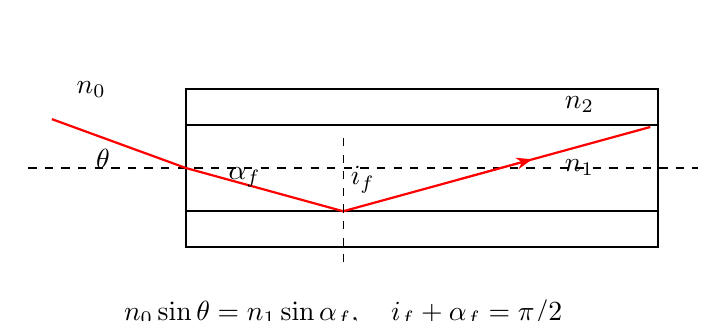
\begin{tikzpicture}
\draw[thick] (0,-1) rectangle(6,1);
\draw[thick] (0,-.55)--(6,-.55); \draw[thick] (0,.55)--(6,.55);
\draw[dashed] (-2,0)--(6.5,0);
\draw[thick,red] (-1.7,.62)--(0,0)--(2,-.55)--(5.9,.52);
\draw[arr,red] (3.5,-.138)--(4.4,.11);
\draw[dashed] (2,-1.2)--(2,.4);
\node at(-1.05,.12) {$\theta$};\node at(.75,-.12) {$\alpha_f$};
\node at(2.25,-.15) {$i_f$};
\node at(5,0) {$n_1$};\node at(5,.8) {$n_2$};\node at(-1.2,1) {$n_0$};
\node at(2,-1.85) {$n_0\sin\theta=n_1\sin\alpha_f,\quad i_f+\alpha_f=\pi/2$};
\end{tikzpicture}
}
\ifdim\wd\diagrambox>.88\linewidth
\sbox{\diagrambox}{\resizebox{.88\linewidth}{!}{\usebox{\diagrambox}}}\fi
\ifdim\ht\diagrambox>.38\textheight
\resizebox{!}{.38\textheight}{\usebox{\diagrambox}}
\else\usebox{\diagrambox}\fi
\par\smallskip{\small 图5b　空气接受角与芯内全反射角\par}\endgroup\end{minipage}\end{center}

图5c中\(V_1,V_2\)为球镜前后顶点，\(C\)为球心，\(I_1\)为仅考虑前曲面所得的中间像，\(F\)为最后焦点。对题给\(n=1.50\)，\(I_1\)在后顶点右侧，因此第二次折射的物是虚物。

\begin{center}
\begin{minipage}{\linewidth}
\centering\begingroup\sbox{\diagrambox}{\small
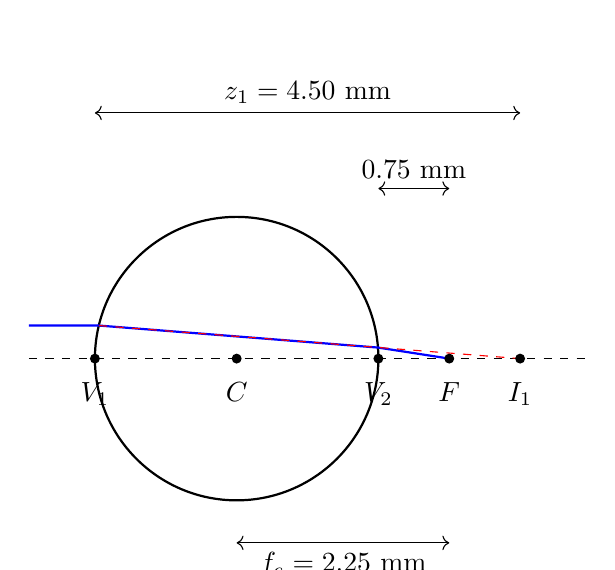
\begin{tikzpicture}[scale=1.2]
\draw[dashed] (-.7,0)--(5.2,0);
\draw[thick] (1.5,0) circle(1.5);
\draw[thick,blue] (-.7,.35)--(.041,.35)--(2.998,.1167)--(3.75,0);
\draw[dashed,red] (.041,.35)--(4.5,0);
\foreach \x/\lab in {0/V_1,1.5/C,3/V_2,3.75/F,4.5/I_1}{
\fill (\x,0) circle(1.5pt); \node[below] at(\x,-.15) {$\lab$};}
\draw[<->] (3,1.8)--(3.75,1.8) node[midway,above] {$0.75\ \mathrm{mm}$};
\draw[<->] (1.5,-1.95)--(3.75,-1.95) node[midway,below] {$f_e=2.25\ \mathrm{mm}$};
\draw[<->] (0,2.6)--(4.5,2.6) node[midway,above] {$z_1=4.50\ \mathrm{mm}$};
\end{tikzpicture}
}
\ifdim\wd\diagrambox>.88\linewidth
\sbox{\diagrambox}{\resizebox{.88\linewidth}{!}{\usebox{\diagrambox}}}\fi
\ifdim\ht\diagrambox>.38\textheight
\resizebox{!}{.38\textheight}{\usebox{\diagrambox}}
\else\usebox{\diagrambox}\fi
\par\smallskip{\small 图5c　两次球面折射的中间像、后焦距与等效焦距\par}\endgroup\end{minipage}\end{center}

原平行光线的高度记为\(h_b\)，对应入射束半径。近轴球镜等效主平面在球心，出射角大小为\(h_b/f_e\)；球镜后表面上的实际光线高度则较小，两者不是同一个高度。

\subsection{四、解题入口}\label{ux56dbux89e3ux9898ux5165ux53e3-4}

第一问先求\(\mathrm{NA}=\sqrt{n_1^2-n_2^2}\)，再用\(\sin\theta_{\max}=\mathrm{NA}/n_0\)。第二问按两个曲面依次求像，不在第一曲面就提前把像当作最终焦点。

第三问用等效焦距\(f_e\)把接受角变成入射光束半径。保持原题近轴精度，采用\(\vartheta\simeq\sin\vartheta\)；若想提高精度，必须把球镜的两次Snell折射也一起改为精确光线，不能只把最后一步换成\(\tan\theta\)就声称得到精确结果。

\subsection{五、解析}\label{ux4e94ux89e3ux6790-4}

\subsubsection{（1）光纤数值孔径与最大接受角}\label{ux5149ux7ea4ux6570ux503cux5b54ux5f84ux4e0eux6700ux5927ux63a5ux53d7ux89d2}

全反射极限满足

\[
\cos\alpha_{f,\max}=\frac{n_2}{n_1}.
\]

故

\[
\sin\alpha_{f,\max}
=\sqrt{1-\frac{n_2^2}{n_1^2}}.
\]

端面Snell定律给

\[
\begin{aligned}
n_0\sin\theta_{\max}
&=n_1\sin\alpha_{f,\max}\\
&=\sqrt{n_1^2-n_2^2}.
\end{aligned}
\]

因此

\[
\boxed{\theta_{\max}
=\arcsin\frac{\sqrt{n_1^2-n_2^2}}{n_0}}.
\]

数值孔径为

\[
\mathrm{NA}
=\sqrt{1.46^2-1.45^2}
=\sqrt{(1.46-1.45)(1.46+1.45)}
=\sqrt{0.0291}.
\]

所以

\[
\mathrm{NA}=0.17058722,
\qquad
\boxed{\theta_{\max}=9.82196^\circ\simeq9.82^\circ}.
\]

这里的角相对于光纤轴，而非相对于芯---包层界面的法线。若\(n_1=n_2\)，数值孔径变成零，光纤不再靠全反射限制非轴向光线；若外部介质改变，最大外部角也随\(n_0\)变化。

\subsubsection{（2）前曲面的中间像}\label{ux524dux66f2ux9762ux7684ux4e2dux95f4ux50cf}

球镜半径为\(a_b=D/2\)。前曲面折射由空气\(n_0\)进入球材\(n\)，曲率中心在右侧，故\(\mathcal R_1=+a_b\)。平行入射等价于物点在\(-\infty\)，所以

\[
\frac{n}{z_1}
=\frac{n-n_0}{a_b}.
\]

得到

\[
\boxed{
z_1=\frac{na_b}{n-n_0}
=\frac{nD}{2(n-n_0)}}.
\]

题给数值为

\[
z_1=\frac{1.50\times3.00}
{2(1.50-1.00)}
=4.50\,\mathrm{mm}.
\]

这个中间像位置相对于前曲面顶点。球厚\(D=3.00\,\mathrm{mm}\)，所以它在后曲面右侧\(1.50\,\mathrm{mm}\)处。

\subsubsection{后曲面的虚物与最终像}\label{ux540eux66f2ux9762ux7684ux865aux7269ux4e0eux6700ux7ec8ux50cf}

相对于后顶点\(V_2\)，第二曲面的物点位置为

\[
z_{\rm obj,2}=z_1-D
=\frac{(2n_0-n)D}{2(n-n_0)}.
\]

本题\(z_{\rm obj,2}=+1.50\,\mathrm{mm}\)，是虚物，因为入射第二曲面的光已经在向右侧该点会聚。

后曲面从\(n\)到\(n_0\)，曲率中心位于左侧，\(\mathcal R_2=-D/2\)。代入统一折射公式，

\[
\frac{n_0}{z_2}
-\frac{n}{z_{\rm obj,2}}
=\frac{n_0-n}{-D/2}.
\]

整理得

\[
\boxed{
z_2=\frac{(2n_0-n)D}{4(n-n_0)}}.
\]

对题给数值，

\[
\boxed{
OF=z_2=\frac{(2-1.5)3.00}{4(1.5-1)}
=0.750\,\mathrm{mm}}.
\]

所求是空气中后顶点到端面的距离。不是\(4.50\,\mathrm{mm}\)的中间像距，也不是\(2.25\,\mathrm{mm}\)的等效焦距。

\subsubsection{用光线矩阵独立检查}\label{ux7528ux5149ux7ebfux77e9ux9635ux72ecux7acbux68c0ux67e5}

前后两曲面的折射功率相同，均为\(2(n-n_0)/D\)。按传播顺序相乘，

\[
\mathsf M=S_2T(D,n)S_1
=\begin{pmatrix}A&B\\C&A\end{pmatrix},
\]

其中

\[
A=\frac{2n_0}{n}-1,\qquad
B=\frac Dn,\qquad
C=-\frac{4n_0(n-n_0)}{nD}.
\]

入射平行光线\((h_b,0)\)在后曲面刚出射时变为

\[
y_2=Ah_b,\qquad
u_2=Ch_b,\qquad
\vartheta_2=\frac{Ch_b}{n_0}.
\]

再在空气中传播距离\(z\)，高度为

\[
y(z)=\left(A+\frac{zC}{n_0}\right)h_b.
\]

焦点条件\(y(z)=0\)给

\[
z=-\frac{n_0A}{C}
=\frac{(2n_0-n)D}{4(n-n_0)}.
\]

与两次折射的结果相同。另一方面，

\[
A^2-BC=1,
\]

验证了矩阵的符号与传播顺序。若误把后曲面曲率取正，\(C\)及焦距都会改变，通常也失去正确的弱折射极限。

\subsubsection{等效焦距和主平面位置}\label{ux7b49ux6548ux7126ux8dddux548cux4e3bux5e73ux9762ux4f4dux7f6e}

外部介质前后相同，矩阵光学给等效焦距

\[
\boxed{
f_e=-\frac{n_0}{C}
=\frac{nD}{4(n-n_0)}}.
\]

本题

\[
f_e=\frac{1.50\times3.00}{4(0.50)}
=2.250\,\mathrm{mm}.
\]

后主平面到后顶点的距离为

\[
f_e-z_2=\frac D2.
\]

所以后主平面经过球心；对称性也使前主平面经过球心。两个主平面在此等效模型中重合，不表示真实光线在球心发生单次折射，而是两曲面系统的近轴等效表示。

\subsubsection{（3）最大平行入射束径}\label{ux6700ux5927ux5e73ux884cux5165ux5c04ux675fux5f84}

设平行入射束直径为\(d_b\)，边缘光线入射高度为\(h_b=d_b/2\)。由矩阵的角度式，

\[
|\vartheta_2|=\frac{h_b}{f_e}.
\]

边缘光线的出射角最大；原理想近轴聚焦中所有光线落在端面轴心，所以保证全部光线被接收的条件为

\[
\frac{d_b}{2f_e}\lesssim\theta_{\max}.
\]

在与球镜近轴近似一致的一阶精度下，\(\theta_{\max}\simeq\sin\theta_{\max}=\mathrm{NA}/n_0\)。因此

\[
\boxed{
d_{b,\max}\simeq2f_e\frac{\mathrm{NA}}{n_0}
=\frac{nD}{2(n-n_0)n_0}
\sqrt{n_1^2-n_2^2}}.
\]

代入未提前舍入的数值孔径，

\[
d_{b,\max}\simeq
2(2.250)(0.17058722)\,\mathrm{mm}
=0.767642\,\mathrm{mm}.
\]

所以近轴设计结果为

\[
\boxed{d_b\lesssim0.77\,\mathrm{mm}}.
\]

若先把\(\sin\theta_{\max}\)取为0.17，得到0.765 mm，常简写为约0.76
mm。这个差别是近轴和中间舍入精度，不宜把末位数字解读成精密制造容差。

\subsubsection{为什么不能用后焦距代替等效焦距}\label{ux4e3aux4ec0ux4e48ux4e0dux80fdux7528ux540eux7126ux8dddux4ee3ux66ffux7b49ux6548ux7126ux8ddd}

后曲面上的光线高度并不等于入射光束半径。对本题，矩阵中\(A=1/3\)，因此

\[
y_2=\frac{h_b}{3}.
\]

从后顶点传播到焦点的距离为\(0.75\,\mathrm{mm}\)，所以出射角也可写成

\[
|\vartheta_2|
\simeq\frac{y_2}{0.75\,\mathrm{mm}}
=\frac{h_b}{2.25\,\mathrm{mm}}.
\]

如果把\(h_b\)直接除以0.75
mm，会把角度放大三倍，并错误地把允许束径缩小三倍。

\subsubsection{近轴结果的精度与模型边界}\label{ux8fd1ux8f74ux7ed3ux679cux7684ux7cbeux5ea6ux4e0eux6a21ux578bux8fb9ux754c}

球镜有限孔径存在球差，不同入射高度的光线不完全在同一轴向位置交会。原题给定近轴条件，因此主答案使用一阶光线模型；它把理想焦点视为零大小，不使用内芯直径来限制束径。

如果改用精确两次Snell折射，应同时考虑出射角与端面上的实际落点。只用\(\tan\theta_{\max}\)代替\(\sin\theta_{\max}\)，而仍保留一阶焦距和``全部光线同焦点''，并不能得到一条完整的精确光学答案。

芯径\(50\,\mu\mathrm m\)与包层外径\(125\,\mu\mathrm m\)描述光纤横向结构。真正的聚焦光斑、球差、衍射与轴向误差会使芯径成为位置容差；原题没有波长和束腰等完整信息，主解不额外计算波动光学耦合效率。

\subsection{六、关键洞察}\label{ux516dux5173ux952eux6d1eux5bdf-4}

光纤耦合是位置与角度的双重筛选。理想同轴近轴模型使位置筛选自动满足，所以束径由数值孔径决定；偏心、离焦或球差会重新激活位置筛选。

球镜的后焦距与等效焦距相差球半径。两个曲面都参与聚焦，后曲面处光线高度也已改变。正确的角度关系来自完整矩阵或两次折射几何，而不是单凭图上画一条三角形。

\subsection{七、易错点}\label{ux4e03ux6613ux9519ux70b9-4}

接受角相对光轴，芯内全反射入射角相对界面法线，二者不能互换。数值孔径是\(n_0\sin\theta_{\max}\)，不是\(\theta_{\max}\)本身。

第二曲面的中间像在右边，是虚物。若使用正实物距的公式，就必须把虚物距取负；本稿采用有符号位置，虚物位置取正。两种定义不可混搭。

等效焦距2.25 mm不能误写成后焦距0.75
mm。保留原题近轴精度时不能把部分三角函数当精确、另一些当一阶而夸大结果精度。

\subsection{八、课堂讲解建议}\label{ux516bux8bfeux5802ux8bb2ux89e3ux5efaux8bae-4}

先把光纤图上的三个角标明，再推数值孔径。球镜部分用一条位置轴写下0、3.00、4.50
mm，虚物的位置一目了然，随后才代符号。

第三问让学生分别从矩阵角度和后曲面高度求出射角，核对二者相同。最后讨论内芯直径为何没有进入理想主答案，再把离焦作为变式，引出位置条件。

\subsection{九、变式训练}\label{ux4e5dux53d8ux5f0fux8badux7ec3-4}

\subsubsection{变式1　球镜折射率改变后的焦点分支}\label{ux53d8ux5f0f1-ux7403ux955cux6298ux5c04ux7387ux6539ux53d8ux540eux7684ux7126ux70b9ux5206ux652f}

外部仍为空气，球径为\(D\)，求什么折射率范围使后顶点外有实焦点，并讨论\(n=2\)和\(n>2\)。

\textbf{解答：} 对\(n>1\)，后焦距

\[
z_2=\frac{(2-n)D}{4(n-1)}.
\]

故\(1<n<2\)时\(z_2>0\)，空气中存在后顶点外实焦点；\(n=2\)时焦点就在后顶点；\(n>2\)时\(z_2<0\)，出射光的近轴交点在后顶点左侧，无法按``端面放在后顶点右侧实焦点''来配置。

\(n\to1^+\)时焦距发散，球镜失去聚焦能力。等效焦距\(f_e=nD/[4(n-1)]\)仍为正，不与负后焦距矛盾，因为主平面位于球内，后焦点可位于主平面右侧而后顶点左侧。

\subsubsection{变式2　精确Snell模型的角度极限}\label{ux53d8ux5f0f2-ux7cbeux786esnellux6a21ux578bux7684ux89d2ux5ea6ux6781ux9650}

保留\(n=1.50,D=3.00\,\mathrm{mm}\)，只求全部边缘光线出射角不超过接受角的精确束径极限，暂不把全部光线同焦点作为假设。

\textbf{解答：}
球半径为\(a_b=D/2\)，入射光线高度\(h_b\)对应第一曲面的入射角

\[
\alpha=\arcsin\frac{h_b}{a_b},\qquad
\beta=\arcsin\left(\frac{n_0}{n}\sin\alpha\right).
\]

球内光线在第二曲面相对法线的入射角仍为\(\beta\)，出射相对法线角为\(\alpha\)，总偏折角为

\[
\theta_{\rm out}=2(\alpha-\beta).
\]

角度边界满足\(2[\alpha-\arcsin((2/3)\sin\alpha)]=\theta_{\max}\)。该函数在允许小孔径区间严格增加，数值解为\(\alpha\simeq0.254072\)
rad。于是

\[
\boxed{
d_{\rm angle}=D\sin\alpha\simeq0.75404\,\mathrm{mm}}.
\]

这是精确球面折射的角度限制，与一阶近轴约0.768
mm有约1.8\%的差异。实际耦合还须在选定端面处逐光线检查落点是否在25
\(\mu\)m芯半径内，不能只凭这个角度极限宣称达到全部光功率耦合。

\subsubsection{变式3　近轴模型中的离焦容差}\label{ux53d8ux5f0f3-ux8fd1ux8f74ux6a21ux578bux4e2dux7684ux79bbux7126ux5bb9ux5dee}

平行入射束径为\(0.600\,\mathrm{mm}\)，光纤端面离开理想焦平面\(\Delta z\)，仍同轴。忽略衍射和球差，求全部光线仍落入50
\(\mu\)m内芯的轴向偏差上限。

\textbf{解答：} 边缘光线的近轴出射角为

\[
\theta_b=\frac{d_b}{2f_e}
=\frac{0.600}{4.500}
=0.133333.
\]

它小于原接受角的一阶值0.170587，方向条件满足。焦平面偏移后，边缘光线高度为\(|y|=|\Delta z|\theta_b\)。芯半径为\(25\,\mu\mathrm m\)，所以

\[
\boxed{
|\Delta z|\le
\frac{25\,\mu\mathrm m}{0.133333}
=187.5\,\mu\mathrm m}.
\]

这是理想几何离焦容差；若有球差、光斑尺寸或偏心，剩余位置裕度应减小。

\par\noindent\begin{minipage}{\linewidth}
\subsubsection{变式4　反求所需芯包折射率差}\label{ux53d8ux5f0f4-ux53cdux6c42ux6240ux9700ux82afux5305ux6298ux5c04ux7387ux5dee}

球镜不变，希望接受直径\(0.500\,\mathrm{mm}\)的平行束。芯折射率仍为\(n_1=1.46\)，在近轴模型中包层折射率最大可以是多少？

\textbf{解答：} 所需接受角一阶值为

\[
\theta_{\rm req}=\frac{d_b}{2f_e}
=\frac{0.500}{4.500}=\frac19.
\]

数值孔径至少为\(n_0\theta_{\rm req}=1/9\)，所以\(n_1^2-n_2^2\ge1/81\)，即

\[
\boxed{
n_2\le\sqrt{1.46^2-\frac1{81}}
\simeq1.45577}.
\]

原包层\(n_2=1.45\)满足要求。减少芯包折射率差会缩小接受角；若包层接近芯折射率，能够输入的束径也趋于零。

\end{minipage}\par
\clearpage

\section{\texorpdfstring{第 6
题　\(\pi\)介子两体衰变与\(\mu\)子的地面存活概率（40
分）}{第 6 题　\textbackslash pi介子两体衰变与\textbackslash mu子的地面存活概率（40 分）}}\label{ux7b2c-6-ux9898-piux4ecbux5b50ux4e24ux4f53ux8870ux53d8ux4e0emuux5b50ux7684ux5730ux9762ux5b58ux6d3bux6982ux738740-ux5206}

宇宙射线中高速飞行的\(\pi\)介子会衰变为\(\mu\)子和\(\mu\)型反中微子：

\[
\pi\longrightarrow\mu+\bar\nu_\mu.
\]

已知静止质量\(m_\pi=139.57061\,\mathrm{MeV}/c^2\)、\(m_\mu=105.65837\,\mathrm{MeV}/c^2\)，反中微子静止质量近似为零。实验室测得\(\pi\)介子速率为\(v=0.965c\)，取\(c=3.00\times10^8\,\mathrm{m/s}\)。

\begin{center}
\begin{minipage}{\linewidth}
\centering\begingroup\sbox{\diagrambox}{\small
\begin{tikzpicture}
\node[draw,circle] (P) at(0,0) {$\pi$静止};
\draw[arr,blue,very thick] (.9,0)--(3,0) node[right] {$\mu:\ E_\mu^*,\,p^*$};
\draw[arr,red,very thick] (-.9,0)--(-3,0) node[left] {$\bar\nu_\mu:\ p^*c,\, -p^*$};
\node at(0,1.5) {$S_*:\quad E_\mu^*+p^*c=m_\pi c^2$};
\draw[arr] (-2,-1.5)--(2,-1.5) node[right] {$S_*$相对$S$以$v$运动};
\node at(0,-2.25) {实验室能量由发射角决定};
\end{tikzpicture}
}
\ifdim\wd\diagrambox>.88\linewidth
\sbox{\diagrambox}{\resizebox{.88\linewidth}{!}{\usebox{\diagrambox}}}\fi
\ifdim\ht\diagrambox>.38\textheight
\resizebox{!}{.38\textheight}{\usebox{\diagrambox}}
\else\usebox{\diagrambox}\fi
\par\smallskip{\small 图6a　母粒子静止系的两体反向动量及实验室系变换\par}\endgroup\end{minipage}\end{center}

（1）求衰变产生的\(\mu\)子的最大速率和最小速率。

（2）这些\(\mu\)子从距地面\(10000\,\mathrm m\)的高空竖直向下飞行。静止\(\mu\)子的半衰期为\(T_{1/2}^{(0)}=1.523\,\mu\mathrm s\)，求地面观察者能够观测到\(\mu\)子的最大概率。

\subsection{一、题型定位}\label{ux4e00ux9898ux578bux5b9aux4f4d-5}

第一问先在母粒子静止系解两体衰变，再作洛伦兹变换。在母粒子静止系，两产物动量大小相同且方向相反；反中微子质量为零，能量等于\(pc\)。这一结构使能量和动量两个守恒条件可以完全求出\(\mu\)子的静止系能量与速率。

衰变方向可以是三维的。最大与最小实验室速率最终出现在正向和反向发射，但必须证明，不能先只挑两根共线光线就认定它们是所有方向中的极值。

第二问求的是\(\mu\)子飞完规定路程之前未衰变的概率，即存活概率。它既受飞行时间影响，又受\(\mu\)子本身的时间膨胀影响。使用的是\(\mu\)子的洛伦兹因子，而不是母\(\pi\)介子的洛伦兹因子。

\subsection{二、知识点}\label{ux4e8cux77e5ux8bc6ux70b9-5}

\subsubsection{1. 两种惯性系}\label{ux4e24ux79cdux60efux6027ux7cfb}

记实验室系为\(S\)，母\(\pi\)介子静止系为\(S_*\)。沿母粒子在实验室的飞行方向取\(x\)轴。\(S_*\)中的量加星号，如\(E_\mu^*,p^*,u^*\)。母粒子速度记为\(\beta_\pi c\)，\(\beta_\pi=0.965\)。

能量单位可先统一为MeV。定义静质量对应的静能

\[
M=m_\pi c^2,\qquad m_0=m_\mu c^2.
\]

这样\(M=139.57061\) MeV、\(m_0=105.65837\)
MeV；若把动量乘\(c\)，它也用MeV表示，避免在质量和能量的平方之间漏掉\(c\)。

\subsubsection{2.
能量---动量关系}\label{ux80fdux91cfux52a8ux91cfux5173ux7cfb}

\(\mu\)子满足

\[
E_\mu^2=(p_\mu c)^2+(m_\mu c^2)^2,
\]

而质量忽略的反中微子满足\(E_\nu=p_\nu c\)。母粒子静止系总动量为零，故两产物动量矢量相反，大小相等。

\subsubsection{3.
半衰期与平均寿命}\label{ux534aux8870ux671fux4e0eux5e73ux5747ux5bffux547d}

存活概率可以写成

\[
P(\tau)=2^{-\tau/T_{1/2}^{(0)}}
=\exp\left(-\frac{\tau}{\tau_0}\right),
\]

其中\(\tau\)是\(\mu\)子沿自身世界线经历的固有时间，平均寿命为

\[
\boxed{\tau_0=\frac{T_{1/2}^{(0)}}{\ln2}}.
\]

半衰期和平均寿命不是同一个时间。若将\(T_{1/2}^{(0)}\)直接放在指数函数的分母，会把概率改变一个\(\ln2\)因子。

\subsection{三、物理图像}\label{ux4e09ux7269ux7406ux56feux50cf-5}

在\(S_*\)中，\(\mu\)子与反中微子的动量一左一右。向实验室母粒子前进方向发射的\(\mu\)子，实验室能量最大；反向发射的能量最小。实验室的母粒子速度远大于\(\mu\)子的静止系速率，反向发射的\(\mu\)子仍然沿实验室前方运动。

\begin{center}
\begin{minipage}{\linewidth}
\centering\begingroup\sbox{\diagrambox}{\small
\begin{tikzpicture}[xscale=3.1,yscale=3.2]
\draw[arr] (-1.1,.52)--(1.3,.52) node[right] {$\cos\vartheta_*$};
\draw[arr] (-1.1,.52)--(-1.1,1.18) node[above] {$E_\mu/E_{\max}$};
\draw[thick,blue,domain=-1:1] plot(\x,{(1+.26188772*\x)/1.26188772});
\fill[red] (-1,.584953) circle(.65pt);\fill[red] (1,1) circle(.65pt);
\node[below] at(-1,.52) {$-1$};\node[below] at(1,.52) {$1$};
\node at(-.45,.86) {$u_{\min}=0.939713c$};
\node[above right] at(.7,1.08) {$u_{\max}=0.979791c$};
\node at(.1,.27) {固定质量：能量越大，速率越大};
\end{tikzpicture}
}
\ifdim\wd\diagrambox>.88\linewidth
\sbox{\diagrambox}{\resizebox{.88\linewidth}{!}{\usebox{\diagrambox}}}\fi
\ifdim\ht\diagrambox>.38\textheight
\resizebox{!}{.38\textheight}{\usebox{\diagrambox}}
\else\usebox{\diagrambox}\fi
\par\smallskip{\small 图6b　发射角改变时的能量与速率范围\par}\endgroup\end{minipage}\end{center}

图6b横轴为\(\cos\vartheta_*\)，其中\(\vartheta_*\)是\(\mu\)子在\(S_*\)中的发射角。能量随这一变量线性增加，而速率由能量决定、单调增加。因此端点就是速率极值。

图6c把实验室路程与\(\mu\)子的固有时间联系。地面和产生点在实验室相距\(h\)，\(\mu\)子飞行时间为\(h/u\)；\(\mu\)子自身钟经历的时间则少一个\(\gamma_\mu\)因子。

\begin{center}
\begin{minipage}{\linewidth}
\centering\begingroup\sbox{\diagrambox}{\small
\begin{tikzpicture}[xscale=1.4,yscale=3.4]
\draw[arr] (0,0)--(5.4,0) node[right] {$h/h_{1/2}$};
\draw[arr] (0,0)--(0,1.18) node[above] {$P$};
\draw[thick,blue,domain=0:5,samples=120] plot(\x,{2^(-\x)});
\draw[dashed] (1,0)--(1,.5)--(0,.5);
\node[left] at(0,.5) {$1/2$};\node[below] at(1,0) {$1$};
\fill[red] (4.47,.04518) circle(.8pt);
\node[above] at(4.2,.22) {10 km：约$4.52\%$};
\node at(2.5,-.4) {$\Delta\tau=h/(\gamma_\mu u)$};
\end{tikzpicture}
}
\ifdim\wd\diagrambox>.88\linewidth
\sbox{\diagrambox}{\resizebox{.88\linewidth}{!}{\usebox{\diagrambox}}}\fi
\ifdim\ht\diagrambox>.38\textheight
\resizebox{!}{.38\textheight}{\usebox{\diagrambox}}
\else\usebox{\diagrambox}\fi
\par\smallskip{\small 图6c　10 km飞行路程、固有时间与存活概率\par}\endgroup\end{minipage}\end{center}

概率最大的\(\mu\)子不是``半衰期最长的某一种粒子''，所有\(\mu\)子的静止半衰期相同；最大概率来自更大的\(\gamma_\mu u\)，使同一实验室路程对应更短固有时间。

\subsection{四、解题入口}\label{ux56dbux89e3ux9898ux5165ux53e3-5}

在母粒子静止系先写

\[
E_\mu^*+p^*c=M,\qquad
(E_\mu^*)^2-(p^*c)^2=m_0^2.
\]

两式联立，得到\(E_\mu^*\)和\(p^*c\)，再由\(u^*/c=p^*c/E_\mu^*\)求速度。实验室极值可以由能量变换证明，再用共线速度合成计算数值。

存活概率最好直接写成固有时间形式

\[
P=2^{-h/(\gamma_\mu uT_{1/2}^{(0)})}.
\]

在接近光速时，不要先把\(u/c\)舍入到三位再计算\(\gamma_\mu\)；\(1-u^2/c^2\)是两个接近的数之差，舍入误差容易放大。

\subsection{五、解析}\label{ux4e94ux89e3ux6790-5}

\subsubsection{（1）母粒子静止系的衰变动量}\label{ux6bcdux7c92ux5b50ux9759ux6b62ux7cfbux7684ux8870ux53d8ux52a8ux91cf}

动量守恒给

\[
\boldsymbol p_\mu^*+\boldsymbol p_\nu^*=0.
\]

因此\(p_\mu^*=p_\nu^*=p^*\)。反中微子能量为\(p^*c\)，总能量守恒为

\[
E_\mu^*+p^*c=M.
\]

由\(\mu\)子能量---动量关系，

\[
(E_\mu^*)^2-(p^*c)^2=m_0^2.
\]

左边作平方差，

\[
(E_\mu^*-p^*c)(E_\mu^*+p^*c)=m_0^2.
\]

第二因子是\(M\)，故第一因子为\(m_0^2/M\)。相加相减后得到

\[
\boxed{E_\mu^*=\frac{M^2+m_0^2}{2M}},
\qquad
\boxed{p^*c=\frac{M^2-m_0^2}{2M}}.
\]

反中微子的能量等于后一项。这里\(M>m_0\)确保\(p^*>0\)；若质量次序相反且没有其他输入能量，母粒子静止系两体衰变不能成立。

\subsubsection{\texorpdfstring{\(\mu\)子的静止系速度}{\textbackslash mu子的静止系速度}}\label{muux5b50ux7684ux9759ux6b62ux7cfbux901fux5ea6}

对有质量粒子，\(u/c=pc/E\)，所以

\[
\boxed{
\beta_*=\frac{u^*}{c}
=\frac{M^2-m_0^2}{M^2+m_0^2}
=\frac{m_\pi^2-m_\mu^2}{m_\pi^2+m_\mu^2}}.
\]

代入数值，

\[
E_\mu^*=109.7782919\,\mathrm{MeV},
\qquad
p^*c=29.7923181\,\mathrm{MeV},
\]

\[
\boxed{\beta_*=0.2713862422}.
\]

检查能量和动量：

\[
109.7782919+29.7923181=139.5706100,
\]

\[
(109.7782919)^2-(29.7923181)^2
=(105.65837)^2.
\]

这个静止系速度明显不能从质量差直接乘\(c\)得到，剩余静能差同时分配到反中微子能量和\(\mu\)子动能。

\subsubsection{任意方向的实验室能量与极值证明}\label{ux4efbux610fux65b9ux5411ux7684ux5b9eux9a8cux5ba4ux80fdux91cfux4e0eux6781ux503cux8bc1ux660e}

在\(S_*\)中，\(\mu\)子的平行、垂直动量分别是

\[
p_x^*=p^*\cos\vartheta_*,
\qquad
p_\perp^*=p^*\sin\vartheta_*.
\]

沿\(x\)方向的洛伦兹变换给

\[
\boxed{
E_\mu(\vartheta_*)
=\gamma_\pi(E_\mu^*+\beta_\pi cp^*\cos\vartheta_*)},
\]

其中\(\gamma_\pi=(1-\beta_\pi^2)^{-1/2}\)。由于\(\beta_\pi,p^*>0\)，实验室能量随\(\cos\vartheta_*\)严格单调增加。

\(\mu\)子的质量不变，实验室速率由

\[
u=c\sqrt{1-\frac{m_0^2}{E_\mu^2}}
\]

决定，并随正能量\(E_\mu\)单调增加。所以最大速率在\(\cos\vartheta_*=1\)，最小速率在\(\cos\vartheta_*=-1\)。这覆盖了全部三维发射方向。

两端均为共线运动，可以使用一维速度合成：

\[
\boxed{
\beta_{\max}=\frac{\beta_\pi+\beta_*}
{1+\beta_\pi\beta_*}},
\]

\[
\boxed{
\beta_{\min}=\frac{\beta_\pi-\beta_*}
{1-\beta_\pi\beta_*}}.
\]

本题\(\beta_\pi>\beta_*\)，最小速度也为正。若母速度小于\(\beta_*\)，后一表达式是负的有符号速度，最小速率应取其绝对值；极值能量法仍有效。

\subsubsection{数值结果及洛伦兹因子核对}\label{ux6570ux503cux7ed3ux679cux53caux6d1bux4f26ux5179ux56e0ux5b50ux6838ux5bf9}

保留中间精度，

\[
\beta_{\max}=0.9797910059,\qquad
\beta_{\min}=0.9397130763.
\]

因此

\[
\boxed{u_{\max}\simeq2.93937\times10^8\,\mathrm{m/s}
\simeq0.980c},
\]

\[
\boxed{u_{\min}\simeq2.81914\times10^8\,\mathrm{m/s}
\simeq0.940c}.
\]

最大速率对应的\(\mu\)子洛伦兹因子为

\[
\boxed{\gamma_{\mu,\max}
=\frac1{\sqrt{1-\beta_{\max}^2}}
=4.9994011}.
\]

也可先算实验室最大能量\(E_{\max}=\gamma_\pi(E_\mu^*+\beta_\pi p^*c)\)，再用\(\gamma_{\mu,\max}=E_{\max}/m_0\)。后一方式避免对接近光速的平方差过早舍入。

\subsubsection{从二维速度变换再检查}\label{ux4eceux4e8cux7ef4ux901fux5ea6ux53d8ux6362ux518dux68c0ux67e5}

速度分量为

\[
u_x=\frac{u^*\cos\vartheta_*+v}
{1+vu^*\cos\vartheta_*/c^2},
\]

\[
u_\perp=\frac{u^*\sin\vartheta_*}
{\gamma_\pi(1+vu^*\cos\vartheta_*/c^2)}.
\]

两分量平方相加，可整理成

\[
1-\frac{u^2}{c^2}
=\frac{(1-\beta_\pi^2)(1-\beta_*^2)}
{(1+\beta_\pi\beta_*\cos\vartheta_*)^2}.
\]

分母在\(\cos\vartheta_*=1\)时最大，故左边最小、速率最大；反向时分母最小、速率最小。它与能量变换的证明一致，并说明不能只变换\(x\)分量后把它误当全部速率。

\subsubsection{（2）存活概率的固有时间}\label{ux5b58ux6d3bux6982ux7387ux7684ux56faux6709ux65f6ux95f4}

实验室中高度为\(h=10000\,\mathrm m\)。某一\(\mu\)子以恒定速率\(u\)竖直向下飞行，忽略空气能量损失、外力加速和重力对速率的微小改变。实验室飞行时间为

\[
\Delta t=\frac hu.
\]

\(\mu\)子沿世界线的固有时间为

\[
\Delta\tau=\frac{\Delta t}{\gamma_\mu}
=\frac{h}{\gamma_\mu u}.
\]

存活概率为

\[
\boxed{
P(u)=2^{-\Delta\tau/T_{1/2}^{(0)}}
=2^{-h/(\gamma_\mu uT_{1/2}^{(0)})}}.
\]

随着\(u\)增加，\(\gamma_\mu u=u/\sqrt{1-u^2/c^2}\)单调增加，因此固有时间减少，存活概率增加。最大概率对应第一问的\(u_{\max}\)。

\subsubsection{最大概率的计算}\label{ux6700ux5927ux6982ux7387ux7684ux8ba1ux7b97}

实验室最短飞行时间为

\[
\Delta t_{\min}
=\frac{10000}{(0.9797910059)(3.00\times10^8)}
=3.40209\times10^{-5}\,\mathrm s.
\]

\(\mu\)子固有时间约为

\[
\Delta\tau_{\min}
=\frac{3.40209\times10^{-5}}{4.9994011}
\simeq6.8050\times10^{-6}\,\mathrm s.
\]

代入半衰期，

\[
\boxed{
P_{\max}
=2^{-10000/
[(4.9994011)(0.9797910059)(3.00\times10^8)(1.523\times10^{-6})]}
\simeq0.04518=4.52\%}.
\]

如果先把最大速率舍入成\(0.980c\)再求时间膨胀因子，会得到约4.59\%的概率。速率的三位有效数字适合最后展示，却不适合在敏感的洛伦兹因子计算中提前使用。

\subsubsection{用平均寿命写成指数式}\label{ux7528ux5e73ux5747ux5bffux547dux5199ux6210ux6307ux6570ux5f0f}

由\(\tau_0=T_{1/2}^{(0)}/\ln2\)，

\[
\tau_0=\frac{1.523}{\ln2}\,\mu\mathrm s
\simeq2.19723\,\mu\mathrm s.
\]

实验室平均寿命为\(\gamma_\mu\tau_0\)。于是

\[
P_{\max}
=\exp\left[-\frac{\Delta t_{\min}}
{\gamma_{\mu,\max}\tau_0}\right].
\]

该指数式与以2为底的半衰期式逐项相同，二者只是参数不同，不能分别使用相同分母。

\subsubsection{\texorpdfstring{在\(\mu\)子静止系用长度收缩核对}{在\textbackslash mu子静止系用长度收缩核对}}\label{ux5728muux5b50ux9759ux6b62ux7cfbux7528ux957fux5ea6ux6536ux7f29ux6838ux5bf9}

对同一恒速\(\mu\)子，可转入它的静止系。地面与产生点在实验室的静止间距为\(h\)，在\(\mu\)子系的同时距离为\(h/\gamma_\mu\)。地面以速度\(u\)向\(\mu\)子接近，所以到达所需时间为

\[
\Delta t'=\frac{h/\gamma_\mu}{u}
=\frac{h}{\gamma_\mu u}.
\]

\(\mu\)子在该系静止，这就是它经历的固有时间。将\(\Delta t'\)代入静止半衰期，得到与实验室计算相同的概率。

不能在同一计算中既把高度缩成\(h/\gamma_\mu\)，又把半衰期扩大成\(\gamma_\mu T_{1/2}^{(0)}\)；那会重复使用一次相对论效应。

\subsubsection{结果的解释与限制}\label{ux7ed3ux679cux7684ux89e3ux91caux4e0eux9650ux5236}

最大存活概率指一个已经产生、向下以最大速率飞行的\(\mu\)子到达地面前仍存在的概率。它不是所有\(\pi\)介子衰变产物落入某个有限探测器的总概率；后者还需发射角分布、探测面积、探测效率等信息。

在没有时间膨胀的错误模型里，飞行时间约34
\(\mu\)s相当于二十多个静止半衰期，概率极小。正确模型把\(\mu\)子所经历的时间减到约6.8
\(\mu\)s，使仍有约百分之几到达地面，这就是高速粒子长距离存活的核心原因。

\subsection{六、关键洞察}\label{ux516dux5173ux952eux6d1eux5bdf-5}

两体衰变在母粒子静止系的产物动量大小固定，角度只是方向变量。实验室能量对\(\cos\vartheta_*\)线性，因此无需对复杂速率根式求导就能找到极值。

衰变规律最自然的时间变量是固有时间。实验室系时间膨胀与\(\mu\)子系长度收缩是同一个世界线间隔的两种描述。

接近光速时，应保留能量或洛伦兹因子中间精度。最后显示\(0.980c\)不表示可以用它替代原数值重新进行概率计算。

\subsection{七、易错点}\label{ux4e03ux6613ux9519ux70b9-5}

反中微子``质量近似为零''不等于能量和动量为零。母粒子静能减去\(\mu\)子静能，也不全是\(\mu\)子动能。

把普通速度相加会得到大于\(c\)的错误结果。任意角度时必须同时变换平行和垂直分量；用能量单调性证明极值更简洁。

飞行过程使用\(\mu\)子的\(\gamma_\mu\)，不是\(\pi\)介子的\(\gamma_\pi\)。半衰期与平均寿命要分清，\(N_t/N_0\)是存活概率而非衰变率。

\subsection{八、课堂讲解建议}\label{ux516bux8bfeux5802ux8bb2ux89e3ux5efaux8bae-5}

先把母粒子系的能量、动量守恒放在同一框内，利用平方差求解，避免展开一串平方根。接着画能量对\(\cos\vartheta_*\)的直线，完成极值证明。

第二问先写固有时间，再选实验室或\(\mu\)子静止系展开。让学生用两种写法核对概率，并比较提前舍入速率造成的差异。

\subsection{九、变式训练}\label{ux4e5dux53d8ux5f0fux8badux7ec3-5}

\subsubsection{变式1　反中微子的实验室能量范围}\label{ux53d8ux5f0f1-ux53cdux4e2dux5faeux5b50ux7684ux5b9eux9a8cux5ba4ux80fdux91cfux8303ux56f4}

求反中微子的最大与最小实验室能量。

\textbf{解答：}
在母粒子静止系，反中微子能量\(E_\nu^*=p^*c=(M^2-m_0^2)/(2M)\)，且动量大小等于能量除以\(c\)。任意方向变换给

\[
E_\nu=\gamma_\pi E_\nu^*(1+\beta_\pi\cos\psi_*).
\]

因此

\[
\boxed{
E_{\nu,\max}=\gamma_\pi E_\nu^*(1+\beta_\pi),\quad
E_{\nu,\min}=\gamma_\pi E_\nu^*(1-\beta_\pi)}.
\]

两端乘积为\((E_\nu^*)^2\)，因为\(\gamma_\pi^2(1-\beta_\pi^2)=1\)。同一次衰变中\(\mu\)子与反中微子方向相反，所以\(\mu\)子最大能量对应反中微子最小能量，不能把两者最大能量同时相加。

\subsubsection{\texorpdfstring{变式2　实验室\(\mu\)子的最大偏离角}{变式2　实验室\textbackslash mu子的最大偏离角}}\label{ux53d8ux5f0f2-ux5b9eux9a8cux5ba4muux5b50ux7684ux6700ux5927ux504fux79bbux89d2}

假设母粒子速度仍为\(0.965c\)，求\(\mu\)子在实验室偏离母飞行方向的最大角。

\textbf{解答：} 动量变换给

\[
\tan\vartheta_{\rm lab}
=\frac{\beta_*\sin\vartheta_*}
{\gamma_\pi(\beta_\pi+\beta_*\cos\vartheta_*)}.
\]

因为\(\beta_\pi>\beta_*\)，分母始终为正，全部\(\mu\)子向前。对\(\vartheta_*\)求导，分子化为\(\beta_\pi\cos\vartheta_*+\beta_*\)，所以极值满足\(\cos\vartheta_*=-\beta_*/\beta_\pi\)。代回得到

\[
\boxed{
\tan\vartheta_{\rm lab,max}
=\frac{\beta_*}
{\gamma_\pi\sqrt{\beta_\pi^2-\beta_*^2}}}.
\]

最大偏离角在母粒子系略偏向后发射的位置，而不在母系垂直发射的位置。与原题速率极值的共线方向是不同的极值目标。

\subsubsection{\texorpdfstring{变式3　最大速率\(\mu\)子的半数到达高度}{变式3　最大速率\textbackslash mu子的半数到达高度}}\label{ux53d8ux5f0f3-ux6700ux5927ux901fux7387muux5b50ux7684ux534aux6570ux5230ux8fbeux9ad8ux5ea6}

求\(\mu\)子以\(u_{\max}\)向下飞行时，存活概率恰为1/2的实验室高度。

\textbf{解答：}
概率\(P=2^{-h/(\gamma_\mu uT_{1/2}^{(0)})}\)。令指数为−1，

\[
\boxed{
h_{1/2}=\gamma_{\mu,\max}u_{\max}T_{1/2}^{(0)}}.
\]

代入\(\gamma_{\mu,\max}=4.9994011\)、\(u_{\max}=0.9797910059c\)，

\[
h_{1/2}\simeq2.238\times10^3\,\mathrm m.
\]

因此10
km约为4.47个``飞行半衰高度''，概率为\(2^{-4.47}\)，与约4.52\%一致。每个粒子的随机衰变时刻不同，这个高度是群体半数存活的统计尺度。

\par\noindent\begin{minipage}{\linewidth}
\subsubsection{变式4　指定存活阈值后的产物比例}\label{ux53d8ux5f0f4-ux6307ux5b9aux5b58ux6d3bux9608ux503cux540eux7684ux4ea7ux7269ux6bd4ux4f8b}

额外假设母粒子静止系衰变方向各向同性。只按能量筛选，求从高度\(h\)沿相同路程飞行时存活概率不低于\(P_c\)的\(\mu\)子占全部产物的比例；暂不考虑探测器角度限制。

\textbf{解答：} 要求

\[
\frac{\gamma_\mu u}{c}
\ge q_c=\frac{h\ln2}
{cT_{1/2}^{(0)}[-\ln P_c]}.
\]

由\(\gamma_\mu u/c=\sqrt{\gamma_\mu^2-1}\)，最低能量为\(E_c=m_0\sqrt{1+q_c^2}\)。各向同性意味着\(\cos\vartheta_*\)在\([-1,1]\)均匀，而实验室能量对此变量线性，故能量在\([E_{\min},E_{\max}]\)均匀。

于是比例为

\[
\boxed{
F_c=
\begin{cases}
1,&E_c\le E_{\min},\\
\dfrac{E_{\max}-E_c}{E_{\max}-E_{\min}},
&E_{\min}<E_c<E_{\max},\\
0,&E_c\ge E_{\max}.
\end{cases}}
\]

其中\(E_{\max/\min}=\gamma_\pi(E_\mu^*\pm\beta_\pi p^*c)\)。这是明确追加各向同性与同路程假设后的条件比例，不是原题有限地面探测器的总计数概率。

\end{minipage}\par
\clearpage

\section{第 7 题　雷电云、电离层光环与高空氦气球（70
分）}\label{ux7b2c-7-ux9898-ux96f7ux7535ux4e91ux7535ux79bbux5c42ux5149ux73afux4e0eux9ad8ux7a7aux6c26ux6c14ux740370-ux5206}

闪电是壮丽的自然现象，近年来还观测到闪电导致的瞬间发光和伽玛射线暴等现象。雷电云通常离地\(6\)---\(12\,\mathrm{km}\)，多数闪电发生在云内，少数到达地面。云内冰状颗粒碰撞后，小冰晶带正电，随气流上浮到云上端；较大颗粒带负电，下坠到云底。云内闪电中和正负电荷，云地闪电把负电荷释放到地面。

\begin{center}
\begin{minipage}{\linewidth}
\centering\begingroup\sbox{\diagrambox}{\small
\begin{tikzpicture}[scale=.85]
\draw[thick,fill=gray!8] (-2,3.5) ellipse(2 and .45);
\draw[thick] (-4,3.5)--(-4,2.1) arc(180:360:2 and .45)--(0,3.5);
\draw[dashed] (-4,2.1) arc(180:0:2 and .45);
\foreach \x in {-3.4,-2.7,-2,-1.3,-.6}{\node[red] at(\x,3.5) {$+$};\node[blue] at(\x,2.1) {$-$};}
\draw[arr] (-2,3.15)--(-2,2.45) node[right] {$E$};
\draw[<->] (.7,2.1)--(.7,3.5) node[midway,right] {$d_c=1\ \mathrm{km}$};
\draw[<->] (-2,4.25)--(0,4.25) node[midway,above] {$R_c=2.5\ \mathrm{km}$};
\draw[thick] (-5,0)--(1.8,0) node[right] {导体地面};
\draw[dashed] (-2,2.1)--(-2,0);
\draw[<->] (-4.7,0)--(-4.7,2.1) node[midway,left] {$h_c=6\ \mathrm{km}$};
\draw[blue,thick] (-2,1.8)--(-2.2,1.5)--(-1.85,1.15)--(-2.15,.8)--(-2,0);
\end{tikzpicture}
}
\ifdim\wd\diagrambox>.88\linewidth
\sbox{\diagrambox}{\resizebox{.88\linewidth}{!}{\usebox{\diagrambox}}}\fi
\ifdim\ht\diagrambox>.38\textheight
\resizebox{!}{.38\textheight}{\usebox{\diagrambox}}
\else\usebox{\diagrambox}\fi
\par\smallskip{\small 图7a　雷电云电荷层及各模型的高度与半径\par}\endgroup\end{minipage}\end{center}

（1）高空气球电场仪测得某圆柱形云内空域的电场均匀，大小为\(0.15\,\mathrm{MV/m}\)。该区域轴线垂直地面，半径\(2.5\,\mathrm{km}\)、高度\(1.0\,\mathrm{km}\)。求上下端电势差、正电荷总量及携带的总电能。取\(\varepsilon_0=8.85\times10^{-12}\,\mathrm{F/m}\)。

（2）起电过程中云上下端电荷随时间指数增加。当地表电场大于\(1.0\,\mathrm{kV/m}\)时会发生云地闪电，地表场很少超过\(10\,\mathrm{kV/m}\)。假设（1）中的雷电云从高空缓慢整体下移，直到负电荷层离地\(6.0\,\mathrm{km}\)时稳定。地面是良导体，估算云正下方地表电场。

（3）云底带负电冰晶尖端放电，先形成厘米量级直径的向下细路径，并使周围空气电离，形成以细路径为轴的粗圆柱形带电体，最终接近地面成为云地闪电通道。通道竖直、负电荷总量为\(2.5\,\mathrm C\)，核心细路径电量相对很小；核心以外内部电场大小相等。通道长度远大于直径，通道直径远大于核心直径，连通云地前的极短时间内电荷分布近似稳定。大气击穿场为\(3.0\,\mathrm{MV/m}\)。估算通道直径并导出核心以外电荷密度的径向分布。

（4）连通后云底及通道负电荷迅速流向地面，温度升至数万摄氏度，空气电离形成等离子体、强光及雷声。电流约\(10\,\mu\mathrm s\)内达到数万安培，通道底部向四周发出约\(30\,\mathrm{kHz}\)强无线电波。低于\(20\,\mathrm{MHz}\)电离层截止频率的电磁波不能进入电离层内部，它会加热离地约\(80\,\mathrm{km}\)的电离层底部；电流超过阈值后，底部瞬间发光，形成以波源正上方位置为中心的光环，最大直径可达数百公里。画出光环产生及扩展的物理过程图，求半径\(100\,\mathrm{km}\)时的径向扩张速度。

（5）球形闪电的微波空泡模型把球闪视为球形等离子体微波空腔。较弱微波不能形成空泡时可向太空辐射并穿透电离层，被卫星观测到；电离层色散会干扰信号，携带探测器的高空气球可在雷电云上方观测。要在离地\(12\,\mathrm{km}\)悬浮载荷为\(50\,\mathrm{kg}\)的氦气球，载荷包含气球材料及探测器，求体积。12
km以下空气温度每升高1 km下降5.0
K；地面\(T_0=290\,\mathrm K\)、\(p_0=1.01\times10^5\,\mathrm{Pa}\)，空气摩尔质量\(M_a=29\,\mathrm{g/mol}\)。12
km处气球内氦气密度为\(\rho_{\rm He}=0.18\,\mathrm{kg/m^3}\)，\(g=9.8\,\mathrm{m/s^2}\)、\(R_g=8.31\,\mathrm{J/(K\cdot mol)}\)。

\subsection{一、题型定位}\label{ux4e00ux9898ux578bux5b9aux4f4d-6}

这道题包含五个相互衔接的模型：云内近似平行板电场、云地系统的镜像电荷、长圆柱电荷的高斯定理、球面波与平面交线的运动，以及变温大气的静力平衡和气球浮力。

每一模型的近似尺度不同。云内场按题设均匀；地表场可先把云两层电荷当成远处点电荷，也可以用均匀圆盘提高几何精度；通道横向尺度只有米量级，长度约6
km，适合忽略端部效应；光环在短时间内可把电离层底面当平面；大气计算则必须保留12
km中的温度变化。

题中电荷``总量''和场强``大小''多为正的标量；有符号电荷密度则必须带负号。以下统一地表竖直向上为\(z\)正方向，通道径向向外为\(r\)正方向，避免把参考答案的方向约定误认为物理矛盾。

\subsection{二、知识点}\label{ux4e8cux77e5ux8bc6ux70b9-6}

\subsubsection{1.
均匀电场的能量}\label{ux5747ux5300ux7535ux573aux7684ux80fdux91cf}

电场能量密度为

\[
w_E=\frac12\varepsilon_0E^2.
\]

对均匀圆柱空间积分，\(U_E=w_E\pi R_c^2d_c\)。平行板等效电容\(C_c=\varepsilon_0\pi R_c^2/d_c\)，电势差\(V_c=Ed_c\)，电荷\(Q_c=C_cV_c\)，同样给\(U_E=Q_cV_c/2\)。

\subsubsection{2.
导体平面的镜像}\label{ux5bfcux4f53ux5e73ux9762ux7684ux955cux50cf}

上半空间一个电荷\(q\)位于高度\(h\)，无限良导体地面的电势为零，可用镜像电荷\(-q\)放在\(-h\)代替地面对外部区域的作用。

地表切向电场为零，法向场由真实电荷和镜像电荷共同贡献。云层不是直接放在地面上的平行板，不能用云内场\(E\)直接当成地表场。

\subsubsection{3.
长圆柱体系的高斯定理}\label{ux957fux5706ux67f1ux4f53ux7cfbux7684ux9ad8ux65afux5b9aux7406}

对长度\(\ell\)、半径\(r\)的同轴高斯柱面，忽略端面通量，

\[
2\pi r\ell E_r(r)=\frac{Q_{\rm enc}(r)}{\varepsilon_0}.
\]

负电通道使\(E_r<0\)，指向轴线。柱面对电荷的积分和通量都要使用有符号量；若全部使用大小，最后应明确把密度大小转换为负密度。

\subsubsection{4.
大气静力平衡}\label{ux5927ux6c14ux9759ux529bux5e73ux8861}

取薄空气层厚\(dz\)，下表面压力与上表面压力之差支撑其重力：

\[
\frac{dp}{dz}=-\rho g.
\]

理想气体密度\(\rho=M_ap/(R_gT)\)，温度按\(T(z)=T_0-\alpha z\)变化，\(\alpha=5.0\times10^{-3}\,\mathrm{K/m}\)。这是静力温度分布，不是将整柱空气当作同一个绝热气团。

\subsection{三、物理图像}\label{ux4e09ux7269ux7406ux56feux50cf-6}

图7b把正、负电荷层及各自镜像同时画出。负层更接近地面，在云下轴线上产生的向上场较强；正层产生较弱的向下场，所以净地表场向上。

\begin{center}
\begin{minipage}{\linewidth}
\centering\begingroup\sbox{\diagrambox}{\small
\begin{tikzpicture}[scale=.8]
\draw[thick] (-3,0)--(3,0) node[right] {$z=0$};
\draw[arr] (-2.8,-3.8)--(-2.8,4.5) node[above] {$z$};
\foreach \y/\q/\lab in {3.8/{+Q_c}/{h_c+d_c},2.5/{-Q_c}/{h_c},-2.5/{+Q_c}/{-h_c},-3.8/{-Q_c}/{-(h_c+d_c)}}{
\draw[fill=gray!10] (0,\y) circle(.22);
\node[right] at(.5,\y) {$\q,\ z=\lab$};
\draw[dashed] (-2.8,\y)--(-.23,\y);
}
\fill (0,0) circle(2pt);
\draw[arr,blue,very thick] (0,.1)--(0,1.3) node[right] {净场向上};
\node at(0,-4.6) {下半空间：等效镜像，上半空间场相同};
\end{tikzpicture}
}
\ifdim\wd\diagrambox>.88\linewidth
\sbox{\diagrambox}{\resizebox{.88\linewidth}{!}{\usebox{\diagrambox}}}\fi
\ifdim\ht\diagrambox>.38\textheight
\resizebox{!}{.38\textheight}{\usebox{\diagrambox}}
\else\usebox{\diagrambox}\fi
\par\smallskip{\small 图7b　地面镜像电荷与地表场方向\par}\endgroup\end{minipage}\end{center}

图7c显示通道场向内、大小恒定，但密度不均匀。半径越大，同一单位长度高斯柱面的面积越大，包围的负电荷量必须按半径增加，故体密度只能按\(1/r\)下降。

\begin{center}
\begin{minipage}{\linewidth}
\centering\begingroup\sbox{\diagrambox}{\small
\begin{tikzpicture}[scale=1.1]
\fill[blue!5] (0,0) circle(1.7);
\draw[thick] (0,0) circle(1.7);
\draw[dashed] (0,0) circle(1.1);
\fill[gray] (0,0) circle(.12);
\foreach \a in {0,60,120,180,240,300}{
\draw[arr,red] ({1.5*cos(\a)},{1.5*sin(\a)})--({.75*cos(\a)},{.75*sin(\a)});}
\draw[<->] (0,-2.15)--(1.7,-2.15) node[midway,below] {$a_{\rm ch}$};
\node at(0,2.3) {$E_r=-E_b$};
\node at(0,-3) {核心$a_0$以外取同轴高斯柱面};
\begin{scope}[shift={(4.5,-1)},xscale=2,yscale=1.4]
\draw[arr] (0,0)--(1.3,0) node[right] {$r/a_{\rm ch}$};
\draw[arr] (0,0)--(0,2) node[above] {$|\rho_q|$};
\draw[thick,blue,domain=.22:1,samples=100] plot(\x,{.4/\x});
\draw[dashed] (.22,0)--(.22,1.82);
\node at(.85,1.65) {$\propto1/r$};
\node at(.6,-.65) {有符号密度为负};
\end{scope}
\end{tikzpicture}
}
\ifdim\wd\diagrambox>.88\linewidth
\sbox{\diagrambox}{\resizebox{.88\linewidth}{!}{\usebox{\diagrambox}}}\fi
\ifdim\ht\diagrambox>.38\textheight
\resizebox{!}{.38\textheight}{\usebox{\diagrambox}}
\else\usebox{\diagrambox}\fi
\par\smallskip{\small 图7c　通道的高斯柱面与负电荷径向分布\par}\endgroup\end{minipage}\end{center}

图7d中无线电波波前始终以\(c\)在三维空间传播，而发光圆环只是球面波与电离层平面的交线。相邻环位置由不同方向的波分别点亮，所以交线速度可以大于\(c\)。

\begin{center}
\begin{minipage}{\linewidth}
\centering\begingroup\sbox{\diagrambox}{\small
\begin{tikzpicture}[scale=.9]
\draw[thick] (-4.5,0)--(4.7,0) node[right] {地面};
\draw[thick] (-4.5,2)--(4.7,2) node[right] {电离层底面};
\draw[blue] (2,0) arc(0:180:2);
\draw[red,thick] (3.2,0) arc(0:180:3.2);
\draw[gray,dashed] (4,0) arc(0:180:4);
\fill (0,0) circle(2pt) node[below] {$O$};
\fill (0,2) circle(2pt) node[above left] {$A$};
\fill (2.498,2) circle(2pt) node[above right] {$B$};
\draw[arr,red] (0,0)--(2.498,2) node[midway,below right] {$ct$};
\draw[<->] (-4.1,0)--(-4.1,2) node[midway,left] {$H_i$};
\draw[<->] (0,1.55)--(2.498,1.55) node[midway,below] {$r_i$};
\draw[arr] (2.55,2.1)--(3.46,2.1);
\node at(.1,4.65) {球面波以$c$传播，交线的径向速度可大于$c$};
\node at(.1,-.8) {$r_i^2+H_i^2=c^2t^2$};
\end{tikzpicture}
}
\ifdim\wd\diagrambox>.88\linewidth
\sbox{\diagrambox}{\resizebox{.88\linewidth}{!}{\usebox{\diagrambox}}}\fi
\ifdim\ht\diagrambox>.38\textheight
\resizebox{!}{.38\textheight}{\usebox{\diagrambox}}
\else\usebox{\diagrambox}\fi
\par\smallskip{\small 图7d　球面波先接触电离层，随后交线扩张\par}\endgroup\end{minipage}\end{center}

图7e把温度、压力及密度随高度下降的趋势与浮力模型放在一起。气球体积取决于外界空气和内部氦气的密度差，不是只用空气密度来支撑50
kg载荷。

\begin{center}
\begin{minipage}{\linewidth}
\centering\begingroup\sbox{\diagrambox}{\small
\begin{tikzpicture}[xscale=.42,yscale=3]
\draw[arr] (0,0)--(13,0) node[right] {$z/\mathrm{km}$};
\draw[arr] (0,0)--(0,1.22) node[above] {归一化量};
\draw[thick,red,domain=0:12] plot(\x,{1-5*\x/290});
\draw[thick,blue,domain=0:12,samples=100] plot(\x,{(1-5*\x/290)^5.8399519});
\draw[dashed] (12,0)--(12,1.1); \node[below] at(12,0) {$12$};
\node[red] at(7,1.1) {$T/T_0$}; \node[blue] at(8,.42) {$\rho/\rho_0$};
\begin{scope}[shift={(21,.2)},xscale=2.38,yscale=.3333]
\draw[thick,fill=blue!8] (0,1.25) ellipse(.9 and 1.1);
\node at(0,1.5) {氦气};
\draw (0,.15)--(0,-.4); \draw[fill=gray!15] (-.35,-.8) rectangle(.35,-.4);
\draw[arr,blue] (0,2.4)--(0,3.5) node[above] {$\rho_bgV_b$};
\draw[arr,red] (.9,1.3)--(.9,.2) node[right] {$\rho_{\rm He}gV_b$};
\draw[arr,red] (0,-.8)--(0,-1.7) node[below] {$m_Lg$};
\end{scope}
\end{tikzpicture}
}
\ifdim\wd\diagrambox>.88\linewidth
\sbox{\diagrambox}{\resizebox{.88\linewidth}{!}{\usebox{\diagrambox}}}\fi
\ifdim\ht\diagrambox>.38\textheight
\resizebox{!}{.38\textheight}{\usebox{\diagrambox}}
\else\usebox{\diagrambox}\fi
\par\smallskip{\small 图7e　线性降温的大气与气球浮力平衡\par}\endgroup\end{minipage}\end{center}

\subsection{四、解题入口}\label{ux56dbux89e3ux9898ux5165ux53e3-6}

为避免符号重复，云半径、层间距、负层高度分别记为\(R_c,d_c,h_c\)，光环层高度记为\(H_i\)，气球高度记为\(z_b\)。数值分别为2.5
km、1.0 km、6.0 km、80 km和12 km。

第（1）问按均匀场模型算\(V_c,Q_c,U_E\)；第（2）问在这些电荷不变的模型下做镜像估算。第（3）问使用通道自身2.5
C电量，不应把云层约26 C电量全部塞入通道。

第（4）问先写交线几何关系再求导；第（5）问先积分大气压强，算出12
km空气密度，再求气球体积。把海平面密度直接代入浮力将严重低估体积。

\subsection{五、解析}\label{ux4e94ux89e3ux6790-6}

\subsubsection{（1）电势差}\label{ux7535ux52bfux5dee}

云上端带正电、下端带负电，云内场从上向下。上端电势高于下端，差值为

\[
V_c=\varphi_{\rm upper}-\varphi_{\rm lower}
=Ed_c.
\]

将\(E=0.15\,\mathrm{MV/m}=1.5\times10^5\,\mathrm{V/m}\)、\(d_c=1000\,\mathrm m\)代入，

\[
\boxed{V_c=1.50\times10^8\,\mathrm V=150\,\mathrm{MV}}.
\]

\subsubsection{正电荷与总电能}\label{ux6b63ux7535ux8377ux4e0eux603bux7535ux80fd}

圆柱横截面积为

\[
A_c=\pi R_c^2=\pi(2500)^2\,\mathrm{m^2}.
\]

平行板近似的面电荷密度大小是\(\sigma_c=\varepsilon_0E\)，所以

\[
\boxed{
Q_c=\varepsilon_0EA_c
=26.0654\,\mathrm C\simeq26\,\mathrm C}.
\]

上端为\(+Q_c\)，下端为\(-Q_c\)；``正电荷总量''不是两端电量大小相加所得的\(2Q_c\)。

能量由场密度积分，

\[
\begin{aligned}
U_E&=\int_{\rm cylinder}\frac12\varepsilon_0E^2\,dV\\
&=\frac12\varepsilon_0E^2A_cd_c
=\frac12Q_cV_c.
\end{aligned}
\]

于是

\[
\boxed{U_E=1.95491\times10^9\,\mathrm J
\simeq2.0\times10^9\,\mathrm J}.
\]

用电容\(C_c=\varepsilon_0A_c/d_c\)计算\(C_cV_c^2/2\)得到同一结果。本问的``总电能''是所给均匀场区域及相应平行板模型的能量，不包含未给出的外部云场或其他云团能量。

\subsubsection{（2）点电荷加镜像的地表场估算}\label{ux70b9ux7535ux8377ux52a0ux955cux50cfux7684ux5730ux8868ux573aux4f30ux7b97}

把每层总电荷集中在其中心：负电荷\(-Q_c\)位于\(z=h_c\)，正电荷\(+Q_c\)位于\(z=h_c+d_c\)。对应镜像分别为\(+Q_c\)在\(-h_c\)、\(-Q_c\)在\(-(h_c+d_c)\)。

位于地面上方的负电荷在原点产生向上场\(Q_c/(4\pi\varepsilon_0h_c^2)\)，下方正镜像也产生同方向同大小场。二者合计

\[
E_{-,z}=\frac{Q_c}{2\pi\varepsilon_0h_c^2}.
\]

上方正层与下方负镜像产生向下场：

\[
E_{+,z}=-\frac{Q_c}
{2\pi\varepsilon_0(h_c+d_c)^2}.
\]

因此

\[
\boxed{
E_{z,\rm point}
=\frac{Q_c}{2\pi\varepsilon_0}
\left[\frac1{h_c^2}
-\frac1{(h_c+d_c)^2}\right]}.
\]

代入\(h_c=6000\,\mathrm m,d_c=1000\,\mathrm m\)，

\[
\boxed{E_{z,\rm point}\simeq
3.455\times10^3\,\mathrm{V/m}
=3.5\,\mathrm{kV/m}},
\]

方向竖直向上。在以向下为正的约定中，它写成负的−3.5 kV/m；方向相同。

这个大小超过题给1.0
kV/m的触发尺度，符合题意中可能发生云地闪电的情形。这里并没有求一个真实的动态放电时刻，因为电荷增长率和下移时间过程未给出。

\subsubsection{均匀圆盘的轴向场：更细的几何估算}\label{ux5747ux5300ux5706ux76d8ux7684ux8f74ux5411ux573aux66f4ux7ec6ux7684ux51e0ux4f55ux4f30ux7b97}

云层半径与高度之比\(R_c/h_c\simeq0.42\)并不极小，点电荷近似有一定误差。现在把上下层均看成半径\(R_c\)、面电荷密度大小\(\sigma_c\)的均匀圆盘。

先求正圆盘在距盘平面\(x>0\)的轴上电势。半径\(s\)、宽\(ds\)的圆环电量为\(dq=2\pi\sigma_cs\,ds\)，到轴上点距离为\(\sqrt{x^2+s^2}\)。故

\[
d\varphi=\frac{dq}
{4\pi\varepsilon_0\sqrt{x^2+s^2}}
=\frac{\sigma_c s\,ds}
{2\varepsilon_0\sqrt{x^2+s^2}}.
\]

从\(s=0\)积分到\(R_c\)，

\[
\varphi(x)=
\frac{\sigma_c}{2\varepsilon_0}
\left(\sqrt{x^2+R_c^2}-x\right).
\]

轴向远离正盘的场大小为

\[
E_{\rm disk}(x)
=-\frac{d\varphi}{dx}
=\frac{\sigma_c}{2\varepsilon_0}
\left(1-\frac{x}{\sqrt{x^2+R_c^2}}\right).
\]

对云的负盘与正盘再分别加入镜像，地表净向上场为

\[
\boxed{
E_{z,\rm disk}
=\frac{\sigma_c}{\varepsilon_0}
\left[
\frac{h_c+d_c}{\sqrt{R_c^2+(h_c+d_c)^2}}
-\frac{h_c}{\sqrt{R_c^2+h_c^2}}
\right]}.
\]

也可用\(\sigma_c=Q_c/(\pi R_c^2)\)替代，系数应为\(Q_c/(\pi\varepsilon_0R_c^2)\)；\(\varepsilon_0\)不可漏掉。

代入题给数据，

\[
\boxed{E_{z,\rm disk}\simeq
2.800\,\mathrm{kV/m}},
\]

仍为向上。与点电荷估算约3.455
kV/m相比，有限圆盘分散电荷使轴上场较弱。均匀圆盘假设改善几何，但仍承接第（1）问的平行板电量估计，不应把它称为真实雷电云的精确结果。

\subsubsection{圆盘结果的远场检验}\label{ux5706ux76d8ux7ed3ux679cux7684ux8fdcux573aux68c0ux9a8c}

当\(R_c\ll h_c\)时，

\[
\frac{x}{\sqrt{x^2+R_c^2}}
=1-\frac{R_c^2}{2x^2}
+O(R_c^4/x^4).
\]

将这个展开代入圆盘式，

\[
E_{z,\rm disk}
\simeq
\frac{Q_c}{2\pi\varepsilon_0}
\left[\frac1{h_c^2}
-\frac1{(h_c+d_c)^2}\right].
\]

正好回到点电荷镜像结果。若还满足\(d_c\ll h_c\)，电场约为\(Q_cd_c/(\pi\varepsilon_0h_c^3)\)，中性电荷双层在远处呈现偶极子场的三次方衰减。

\subsubsection{（3）通道线电荷与直径}\label{ux901aux9053ux7ebfux7535ux8377ux4e0eux76f4ux5f84}

通道长度近似为负云层离地高度\(h_c=6000\,\mathrm m\)，负电荷总量大小为\(Q_{\rm ch}=2.5\,\mathrm C\)。有符号线电荷密度为

\[
\lambda_{\rm ch}=-\frac{Q_{\rm ch}}{h_c},
\]

大小为

\[
|\lambda_{\rm ch}|
=4.16667\times10^{-4}\,\mathrm{C/m}.
\]

对通道外\(r>a_{\rm ch}\)的高斯柱面，

\[
E_r(r)=\frac{\lambda_{\rm ch}}
{2\pi\varepsilon_0r}<0.
\]

通道边缘场的大小取击穿场\(E_b=3.0\times10^6\,\mathrm{V/m}\)，

\[
E_b=\frac{|\lambda_{\rm ch}|}
{2\pi\varepsilon_0a_{\rm ch}}.
\]

故通道直径为

\[
\boxed{
D_{\rm ch}=2a_{\rm ch}
=\frac{Q_{\rm ch}}
{\pi\varepsilon_0E_bh_c}
\simeq4.995\,\mathrm m
\simeq5.0\,\mathrm m}.
\]

几米通道与几厘米核心、几千米长度之间有清楚的尺度分离，符合题给近似。若误把云正电总量26
C代入，会把直径放大约十倍。

\subsubsection{核心外的电荷密度}\label{ux6838ux5fc3ux5916ux7684ux7535ux8377ux5bc6ux5ea6}

题设核心外通道内部电场大小相同，方向向内，因此

\[
E_r(r)=-E_b,
\qquad a_0<r<a_{\rm ch}.
\]

由柱坐标散度形式的高斯定理，

\[
\frac1r\frac{d}{dr}[rE_r(r)]
=\frac{\rho_q(r)}{\varepsilon_0}.
\]

代入恒定的\(E_r=-E_b\)，

\[
\frac1r\frac{d(-E_br)}{dr}
=-\frac{E_b}{r}.
\]

所以

\[
\boxed{\rho_q(r)=-\frac{\varepsilon_0E_b}{r}}.
\]

其中\(\rho_q\)单位为\(\mathrm{C/m^3}\)，不是空气质量密度。其大小为\(\varepsilon_0E_b/r\)；负号表达通道带负电，不能被当作可省略的数学符号。

\subsubsection{用积分再检查密度}\label{ux7528ux79efux5206ux518dux68c0ux67e5ux5bc6ux5ea6}

把核心理想化到极小半径，半径\(r\)内单位长度的电量为

\[
\lambda(r)=\int_0^r
\rho_q(s)\,2\pi s\,ds
=-2\pi\varepsilon_0E_br.
\]

因此高斯柱面给

\[
E_r(r)=\frac{\lambda(r)}
{2\pi\varepsilon_0r}=-E_b,
\]

与假设一致。虽然密度按\(1/r\)形式增大，柱壳体积微元正比\(r\,dr\)，总电量仍有限。

物理核心不能真的取\(r=0\)并继续使用此密度，题设明确排除了核心。若核心半径为\(a_0\)，要使其外侧场已经为\(-E_b\)，核心单位长度电量应约为\(-2\pi\varepsilon_0E_ba_0\)，仅占全部通道电量的\(a_0/a_{\rm ch}\)，可以很小。

这个模型描述稳定的体电荷分布，不是静电平衡的理想金属柱。理想导体内部电场为零，而题目明确规定内部非零电场，不能把电荷全放在表面。

\subsubsection{（4）电离层光环出现与扩张}\label{ux7535ux79bbux5c42ux5149ux73afux51faux73b0ux4e0eux6269ux5f20}

按题设把电离层底面取为离地\(H_i=80\,\mathrm{km}\)的平面。无线电波从地面点\(O\)在\(t=0\)发出，波前球面半径为\(ct\)。最早到达正上方\(A\)，时间为

\[
t_A=\frac{H_i}{c}.
\]

在\(t\ge t_A\)时，球面与电离层平面的交线为圆，环半径\(r_i\)满足

\[
H_i^2+r_i^2=(ct)^2.
\]

故

\[
\boxed{r_i(t)=\sqrt{c^2t^2-H_i^2}}.
\]

若改用从光环首次出现起的时间\(\tau=t-t_A\)，

\[
r_i(\tau)=\sqrt{2H_ic\tau+c^2\tau^2}.
\]

两种时间原点不能混用：以发射为零必须保留\(t_A\)，以首次出现为零则平方中有交叉项。

\subsubsection{径向速度}\label{ux5f84ux5411ux901fux5ea6}

对几何式求导，

\[
2r_i\frac{dr_i}{dt}=2c^2t.
\]

于是

\[
\boxed{
v_{\rm ring}=\frac{dr_i}{dt}
=\frac{c^2t}{r_i}
=c\frac{\sqrt{H_i^2+r_i^2}}{r_i}}.
\]

取\(H_i=80\,\mathrm{km}\)、\(r_i=100\,\mathrm{km}\)，

\[
v_{\rm ring}
=c\sqrt{1+\left(\frac{80}{100}\right)^2}
=1.28062485c.
\]

所以

\[
\boxed{v_{\rm ring}\simeq3.842\times10^8\,\mathrm{m/s}}.
\]

在该半径的到达时刻\(t=\sqrt{80^2+100^2}\,\mathrm{km}/c\simeq0.42688\,\mathrm{ms}\)，首次出现时刻约0.26667
ms，扩张到100 km历时约0.16021 ms。

\subsubsection{几何速度超过光速的含义}\label{ux51e0ux4f55ux901fux5ea6ux8d85ux8fc7ux5149ux901fux7684ux542bux4e49}

交线速度并不是无线电波的传播速度，也不是电离层物质的径向运动速度。半径不同的位置分别由从\(O\)沿不同方向发出的波点亮，外侧位置不需要先等待内侧发光后才接到信息。

在\(r_i\to0^+\)时，理想交线速度趋于无穷；它对应球面与平面相切时交点对半径的敏感性，不表示无限快的信息传输。有限波包宽度、电离层厚度及发光反应时间会使实际边缘模糊，题目未给这些参数。

另一种几何表达为\(v_{\rm ring}=c/\cos\theta_i\)，其中\(\cos\theta_i=r_i/\sqrt{H_i^2+r_i^2}\)。分母是斜程\(OB\)，不能误写成竖直高度\(OA\)。

\subsubsection{（5）12 km的温度}\label{kmux7684ux6e29ux5ea6}

温度梯度为

\[
\alpha=5.0\,\mathrm{K/km}
=5.0\times10^{-3}\,\mathrm{K/m}.
\]

取\(z_b=12000\,\mathrm m\)，

\[
\boxed{T_b=T_0-\alpha z_b=290-60=230\,\mathrm K}.
\]

该温度分布只在题给12 km以下使用，不向任意高度延伸到零或负绝对温度。

\subsubsection{积分大气静力方程}\label{ux79efux5206ux5927ux6c14ux9759ux529bux65b9ux7a0b}

由

\[
\frac{dp}{dz}
=-\rho g
=-\frac{M_ag}{R_g[T_0-\alpha z]}p,
\]

分离变量，

\[
\frac{dp}{p}
=-\frac{M_ag}{R_g}
\frac{dz}{T_0-\alpha z}.
\]

从地面\(z=0,p=p_0\)积分至\(z,p(z)\)：

\[
\ln\frac{p(z)}{p_0}
=-\frac{M_ag}{R_g}
\int_0^z\frac{ds}{T_0-\alpha s}.
\]

积分为

\[
\int_0^z\frac{ds}{T_0-\alpha s}
=-\frac1\alpha
\ln\frac{T_0-\alpha z}{T_0}.
\]

因此

\[
\boxed{
p(z)=p_0
\left(1-\frac{\alpha z}{T_0}\right)^{q_a}},
\qquad
q_a=\frac{M_ag}{\alpha R_g}.
\]

这里\(q_a\)无量纲。两个负号相消后，对数右侧仍是负值，因为温度比小于1，故压力随高度降低，方向正确。

\subsubsection{空气密度分布}\label{ux7a7aux6c14ux5bc6ux5ea6ux5206ux5e03}

地面密度为

\[
\rho_0=\frac{M_ap_0}{R_gT_0}.
\]

用\(T(z)=T_0(1-\alpha z/T_0)\)，

\[
\begin{aligned}
\rho(z)
&=\frac{M_ap(z)}{R_gT(z)}\\
&=\rho_0
\left(1-\frac{\alpha z}{T_0}\right)^{q_a-1}.
\end{aligned}
\]

所以

\[
\boxed{
\rho(z)=\frac{M_ap_0}{R_gT_0}
\left(1-\frac{\alpha z}{T_0}\right)^{
M_ag/(\alpha R_g)-1}}.
\]

密度指数比压力指数小1，因为温度也随高度下降。若在密度式中仍使用\(q_a\)，就漏掉了分母温度的变化。

\subsubsection{数值代入}\label{ux6570ux503cux4ee3ux5165}

用\(M_a=0.029\,\mathrm{kg/mol}\)，

\[
q_a=\frac{0.029\times9.8}{0.005\times8.31}
=6.8399519.
\]

12 km处

\[
p_b=1.01\times10^5
\left(\frac{230}{290}\right)^{6.8399519}
=2.0689134\times10^4\,\mathrm{Pa}.
\]

进而

\[
\boxed{
\rho_b=\frac{0.029p_b}{8.31\times230}
=0.3139146\,\mathrm{kg/m^3}}.
\]

密度单位是\(\mathrm{kg/m^3}\)。若误写成\(\mathrm{kg/cm^3}\)，相差百万倍，不能仅因数字0.31看起来合理就忽略单位。

\subsubsection{浮力平衡求气球体积}\label{ux6d6eux529bux5e73ux8861ux6c42ux6c14ux7403ux4f53ux79ef}

题给50
kg载荷不包括氦气质量，但包括气球材料与探测器。设气球体积为\(V_b\)，外界浮力为\(\rho_bgV_b\)，氦气重力为\(\rho_{\rm He}gV_b\)，载荷重力为\(m_Lg\)。

悬浮条件为

\[
\rho_bgV_b=\rho_{\rm He}gV_b+m_Lg.
\]

消去\(g\)，

\[
\boxed{V_b=\frac{m_L}{\rho_b-\rho_{\rm He}}}.
\]

必须有\(\rho_b>\rho_{\rm He}\)；若密度差为零或负，无有限正体积能够托起正载荷。

代入题给氦气密度0.18 kg/m³及未舍入的空气密度，

\[
\boxed{
V_b=\frac{50}{0.3139146-0.18}
=373.37\,\mathrm{m^3}
\simeq3.7\times10^2\,\mathrm{m^3}}.
\]

若先把空气密度近似成0.31 kg/m³，结果为384.6
m³，常写约\(3.8\times10^2\,\mathrm{m^3}\)。密度差比单个密度小，提前舍入会在体积上放大。

用质量直接检验：题给氦气质量约为\(0.18V_b=67.21\)
kg，排开空气质量约为\(0.3139146V_b=117.21\) kg，差为50
kg，正好支撑载荷。

\subsubsection{氦气条件与大气条件的区分}\label{ux6c26ux6c14ux6761ux4ef6ux4e0eux5927ux6c14ux6761ux4ef6ux7684ux533aux5206}

原题把12 km处氦气密度直接给定为0.18
kg/m³，主解按这一条件使用，不额外假设球内与外界等压、同温来替换它。氦气密度的物理值取决于内部压力与温度，外界空气密度则由题给静力温度分布求得。

若另规定柔性球囊、内外等压同温，应以氦气摩尔质量重新求内部密度，体积将不同；这是变式中的另一个模型，而不是原题可无条件加入的假设。

\par\noindent\begin{minipage}{\linewidth}
\subsubsection{大气积分的等温极限}\label{ux5927ux6c14ux79efux5206ux7684ux7b49ux6e29ux6781ux9650}

当温度梯度趋于零时，压力表达式看似指数\(q_a\to\infty\)，但可以取对数：

\[
\ln\frac{p(z)}{p_0}
=\frac{M_ag}{\alpha R_g}
\ln\left(1-\frac{\alpha z}{T_0}\right).
\]

利用\(\ln(1-u)=-u+O(u^2)\)，

\[
\ln\frac{p(z)}{p_0}\longrightarrow
-\frac{M_agz}{R_gT_0}.
\]

所以回到熟悉的等温大气公式\(p=p_0e^{-M_agz/(R_gT_0)}\)。这项极限同时核对了变温积分的指数、符号与初始条件。

\end{minipage}\par
\subsection{六、关键洞察}\label{ux516dux5173ux952eux6d1eux5bdf-6}

云内与地表是两个不同几何区域，均匀云场不能直接搬到地表。导体镜像使轴上法向场加倍，两层正负电荷的远场又部分抵消。

恒定径向场并不对应均匀体密度，而对应\(\rho_q\propto1/r\)。密度符号、核心截断和积分总量共同决定这个模型是否自洽。

超光速光环是几何交线，不是物质或信号沿环面传播。气球的承载能力则由密度差决定，不能把50
kg与总排空气质量直接相等。

\subsection{七、易错点}\label{ux4e03ux6613ux9519ux70b9-6}

云电量约26 C、通道电量2.5
C是两个不同数据。微伏、兆伏、公里等单位必须先统一；电势差是150
MV而不是150 kV。

镜像电荷符号与真实电荷相反，地表法向场不是相互抵消。圆盘展开式的\(\varepsilon_0\)不可丢失。负通道有符号密度应带负号。

光环初次出现有延迟\(H_i/c\)，不能从\(t=0\)就写\(r_i=ct\)。温度下降需按K/m换算；空气密度单位是kg/m³。载荷不含氦气时必须扣去氦气重力。

\subsection{八、课堂讲解建议}\label{ux516bux8bfeux5802ux8bb2ux89e3ux5efaux8bae-6}

用五个小模型分段板书，每个模型先说明研究区域、坐标方向及给定数据。地表场部分先作点电荷镜像，再用圆环积分让学生看见近似如何改善，并检查远场极限。

通道部分同时写有符号Gauss方程与场强大小，强调负密度。光环用球面切平面的动态图像解释交线速度，避免把结果大于\(c\)直接判错。气球部分让学生先估量压力和密度下降，再积分，最后核对排开空气质量减去氦气质量等于50
kg。

\subsection{九、变式训练}\label{ux4e5dux53d8ux5f0fux8badux7ec3-6}

\subsubsection{变式1　指数起电与电能增长}\label{ux53d8ux5f0f1-ux6307ux6570ux8d77ux7535ux4e0eux7535ux80fdux589eux957f}

云几何保持不变，电量\(Q_c(t)=Q_0e^{t/\tau_c}\)。最初地表场大小为0.50
kV/m，求达到1.0 kV/m所需时间和云电能增长倍数。

\textbf{解答：}
点电荷或均匀圆盘模型的场都对电量线性，故\(E_{\rm ground}(t)=E_0e^{t/\tau_c}\)。达到两倍场强时

\[
\boxed{t_{\rm th}=\tau_c\ln2}.
\]

几何电容不变，电能\(U=Q_c^2/(2C_c)\)，所以场增加两倍时电量增加两倍，电能增加四倍。能量不是按同一个\(e^{t/\tau_c}\)增长，而是\(e^{2t/\tau_c}\)。

\subsubsection{变式2　有限核心的电量与通道储能}\label{ux53d8ux5f0f2-ux6709ux9650ux6838ux5fc3ux7684ux7535ux91cfux4e0eux901aux9053ux50a8ux80fd}

核心半径为\(a_0\)，外半径为\(a_{\rm ch}\)，核心外\(E_r=-E_b\)。求核心所需线电量、壳层线电量以及壳层单位长度场能。

\textbf{解答：} 在\(r=a_0\)处应用Gauss定理，核心线电量必须为

\[
\boxed{\lambda_0=-2\pi\varepsilon_0E_ba_0}.
\]

壳层密度仍为\(-\varepsilon_0E_b/r\)，积分得

\[
\lambda_{\rm shell}
=-2\pi\varepsilon_0E_b(a_{\rm ch}-a_0).
\]

两者相加为\(-2\pi\varepsilon_0E_ba_{\rm ch}\)，与边缘场一致。壳层单位长度场能为

\[
\boxed{
\frac{U_{\rm shell}}{\ell}
=\int_{a_0}^{a_{\rm ch}}\frac12\varepsilon_0E_b^2\,2\pi r\,dr
=\frac{\pi\varepsilon_0E_b^2}{2}
(a_{\rm ch}^2-a_0^2)}.
\]

若只保留壳层电量而把核心严格设为零，场在\(a_0\)附近便不再是恒定\(E_b\)；``核心电量相对很小''不等于在所有边界条件中严格为零。

\subsubsection{变式3　有限波包引起的光环宽度}\label{ux53d8ux5f0f3-ux6709ux9650ux6ce2ux5305ux5f15ux8d77ux7684ux5149ux73afux5bbdux5ea6}

无线电波包持续\(\Delta t=10\,\mu\mathrm s\)，忽略发光延迟及层厚。在环半径100
km时估算发光环的径向宽度。

\textbf{解答：}
波包前沿与后沿到达同一高度平面的时刻相差\(\Delta t\)。在\(\Delta t\)远小于扩张时间尺度时，径向宽度约为

\[
\Delta r_i\simeq\frac{dr_i}{dt}\Delta t.
\]

使用主问题的\(v_{\rm ring}=1.28062485c\)，

\[
\boxed{
\Delta r_i\simeq
(3.84187\times10^8)(10^{-5})
=3.84\,\mathrm{km}}.
\]

它大于自由空间波包厚度\(c\Delta t=3.00\)
km，因为光环是波包与平面的斜交投影。接近首次相切时线性宽度近似失效，应分别计算两条波前的\(r_i(t)\)再作差。

\par\noindent\begin{minipage}{\linewidth}
\subsubsection{变式4　另规定内外等压同温的柔性气球}\label{ux53d8ux5f0f4-ux53e6ux89c4ux5b9aux5185ux5916ux7b49ux538bux540cux6e29ux7684ux67d4ux6027ux6c14ux7403}

在12
km处另规定氦气与空气等温、等压，氦气摩尔质量为\(4.00\,\mathrm{g/mol}\)，载荷仍为50
kg。求气球体积，并说明与原题数据的关系。

\textbf{解答：} 理想气体在相同\(p,T\)下密度之比等于摩尔质量之比：

\[
\rho_{\rm He,new}=\frac4{29}\rho_b
\simeq0.0432986\,\mathrm{kg/m^3}.
\]

于是

\[
\boxed{
V_{\rm new}
=\frac{50}{\rho_b(1-4/29)}
\simeq184.76\,\mathrm{m^3}}.
\]

此结果比原题按给定0.18 kg/m³求出的373.37
m³小，因为内部氦气质量更小。两个计算采用不同内部气体条件，不能把本变式的等压同温假设倒加到原题中，替换其明确给定的氦气密度。
\end{minipage}\par

\end{document}
